% !BIB TS-program = biber

% This is the root file of your thesis: thesis.tex
% A line starting with % is a comment. In some cases, I have included a command preceded by a %. You may activate the command by removing the %.

%%===================================
\documentclass[12pt]{report}
\usepackage{ramsstyle}
\usepackage{listings}
\usepackage{graphicx}
\usepackage{float}
\usepackage{caption}
\usepackage{subcaption}
\usepackage{gensymb}

\usepackage{import}
\usepackage{pax}
\usepackage{pdfpages}
\usepackage{minitoc}
\usepackage{multirow, tabularx}
\usepackage{pgfplots}

%\usepackage{showframe}
%%===================================
%Write the various parts of your thesis as separate files and include them into the main file by the command \include{name of included file}. When you compile the LaTeX file, you may choose which subfiles to include by the command

%\includeonly{sections/methodology/methodology}
%%===================================
\begin{document}

\cleardoublepage
\pagenumbering{roman}
\setcounter{page}{5}
%% !TEX encoding = UTF-8 Unicode
%!TEX root = thesis.tex
% !TEX spellcheck = en-US
 
%This is the Titlepage
%%=========================================
\thispagestyle{empty}

\includegraphics[scale=0.4]{fig/logo.png}
\mbox{}\\[6pc]
\begin{center}
\Huge{Open source JavaScript voxelization library, with complementary applications}\\[2pc]
 
\Large{André Storhuag}\\[1pc]
\large{May 2020}\\[2pc]
 
PROJECT / BACHELOR'S THESIS\\
Department of ICT and Natural Sciences\\
Norwegian University of Science and Technology
\end{center}
\vfill
 
\noindent Supervisor 1: Ricardo Da Silva Torres

\noindent Supervisor 2: Saleh Abdel-Afou Alaliyat
  % This is the titlepage
%Egenerklæring
%%=========================================

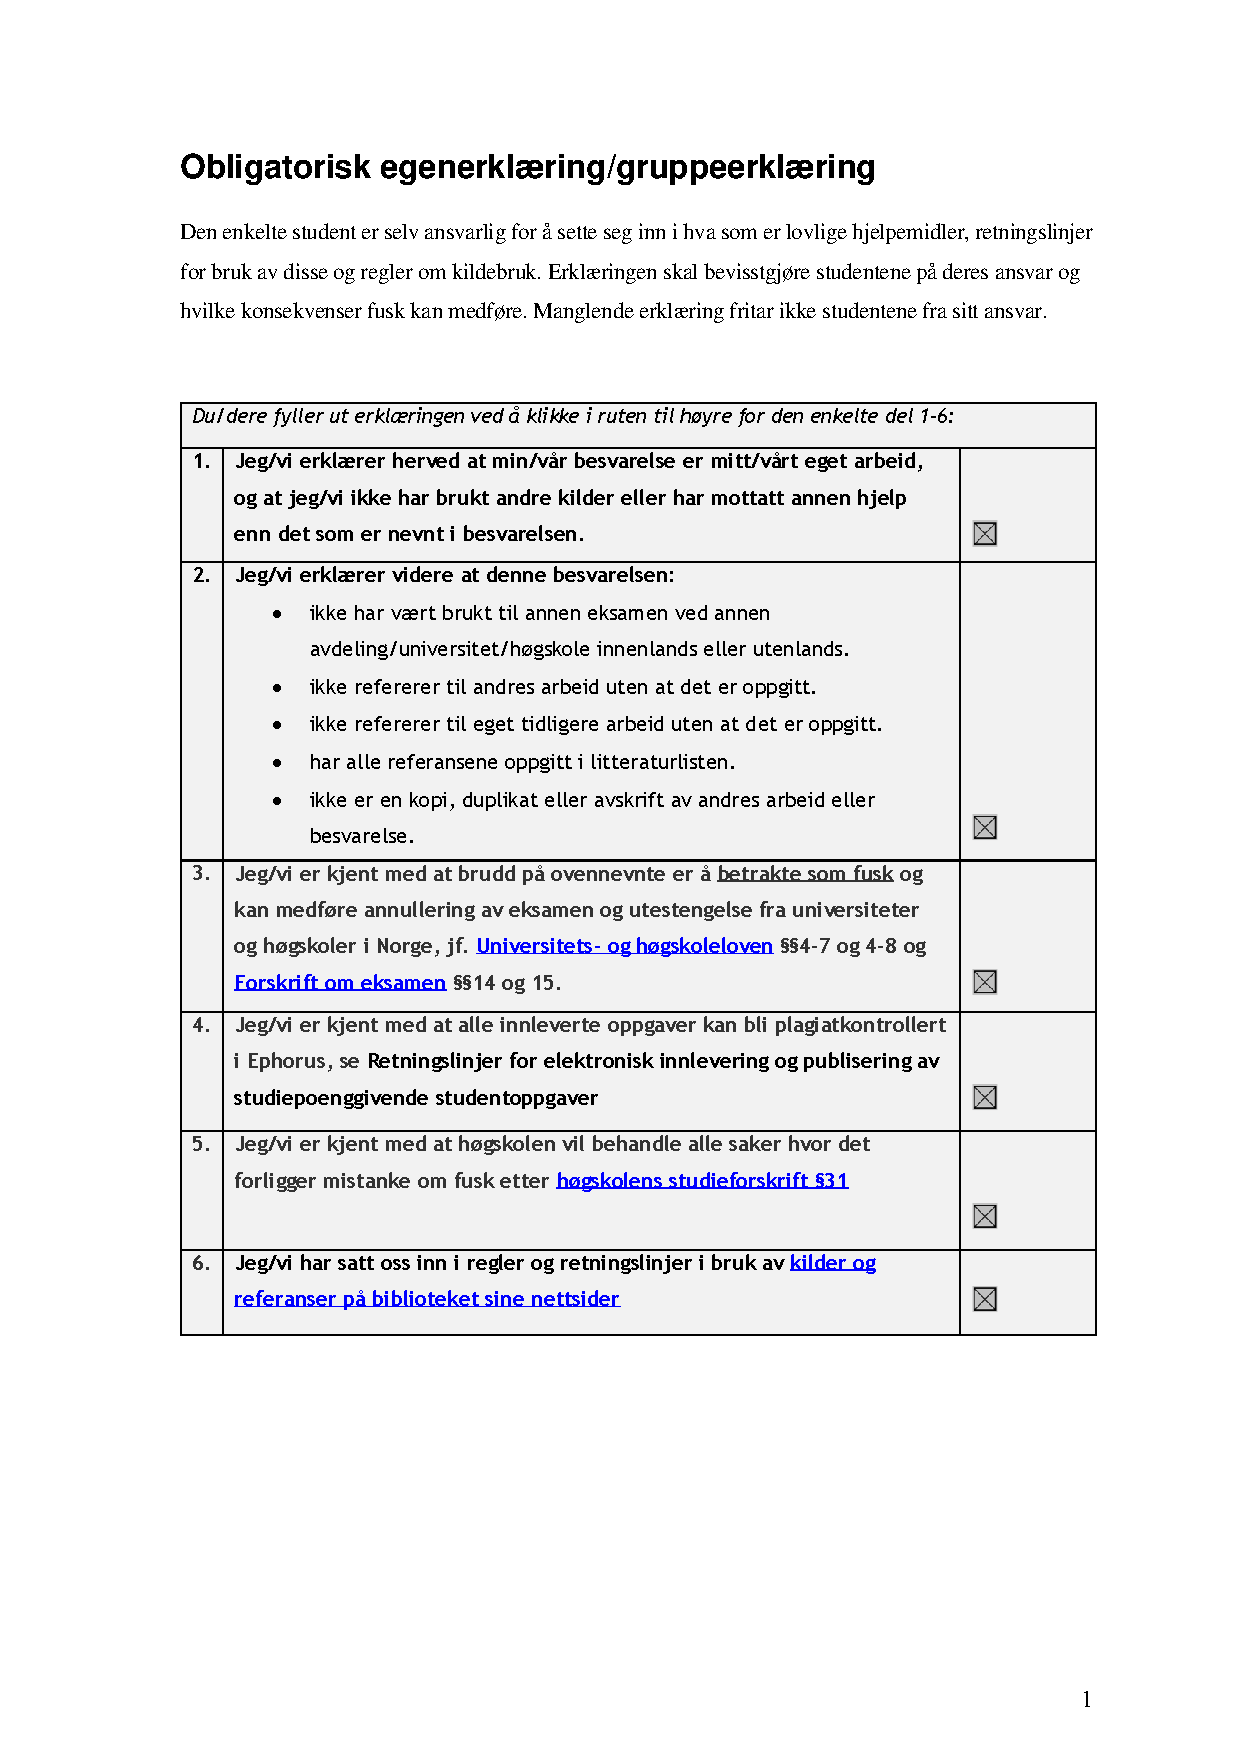
\includepdf[pages=1, pagecommand={}]{sections/_meta/bachelor-egenerklering.pdf}

%This is the Abstract
%%=========================================
\section*{Abstract}
Voxelization is the process of converting 3D models into volumetric data. The main goal of this thesis is to improve the the open-source Voxelizer engine, which is written in JavaScript. To make voxelization easy and available, a complementary cross-platform desktop application is also developed, making use of the Voxelizer engine. Further, to make the software secure and easy to maintain, this thesis also focus on automation. A GitHub Action named JSDoc Action is developed for the purpose of automating the generation of JSDoc documentation. The result of this thesis includes a maintainable and easy to use collection of high-quality voxelization software, in addition to several automation tools.

%Here you give a summary of your your work and your results. This is like a management summary and should be written in a clear and easy language, without many difficult terms and without abbreviations. Everything you present here must be treated in more detail in the main report. You should not give any references to the report in the summary -- just explain what you have done and what you have found out. The Summary and Conclusions should be no more than two pages.

%This is the Abstract
%%=========================================
\section*{Sammendrag}
Voxelisering er prosessen å konvertere 3D-modeller til volumetrisk data. Hovedmålet med denne oppgaven er å forbedre open-source Voxelizer-motoren, som er skrevet i JavaScript. For å gjøre voxelisering enkelt og tilgjengelig, er det også utviklet en plattformuavhengig desktop-applikasjon som benytter seg av Voxelizer-motoren. For å gjøre programvaren sikker og enkel å vedlikeholde, fokuserer denne rapporten også på automatisering. En GitHub Action kalt JSDoc Action er utviklet for å automatisere genereringen av JSDoc dokumentasjon. Resultatet av denne oppgaven inkluderer en vedlikeholdbar og brukervennlig samling av høykvalitets voxeliserings-programvare, i tillegg til flere automatiseringsverktøy.

%Here you give a summary of your your work and your results. This is like a management summary and should be written in a clear and easy language, without many difficult terms and without abbreviations. Everything you present here must be treated in more detail in the main report. You should not give any references to the report in the summary -- just explain what you have done and what you have found out. The Summary and Conclusions should be no more than two pages.

%This is the Acknowledgement
%%=========================================
\section*{Acknowledgement}
I wish to express my deepest gratitude to my supervisor, Professor Ricardo da Silva Torres, for all the help and guidance throughout the entire project. I also want to acknowledge all the love and support from my family - my parents, Synnøve and Ove; and my sisters, Maria, Viktoria and Helene. They all kept me going, and this work would not have been possible without them.
\begin{flushright}
    André Storhaug, \r{A}lesund 20.05.2020
\end{flushright}
%%This is the Preface
%%=========================================
\addcontentsline{toc}{section}{Preface}
\section*{Preface}

This bachelor thesis is written a student from Computer Engineering at NTNU Ålesund ....\\

This type of technology.... \\

What intrigued us ... 
\tableofcontents
\addcontentsline{toc}{chapter}{\listfigurename}
\listoffigures
\addcontentsline{toc}{chapter}{\listtablename}
\listoftables
\addcontentsline{toc}{chapter}{\lstlistlistingname}
\lstlistoflistings
%This is Appendix A - Acronyms
%%=========================================
\addcontentsline{toc}{chapter}{Terminology}
\chapter*{Terminology} % Terminologi
\begin{description}
\section*{Glossary} % Gloser
\item[Cross-platform software] Computer software that can be run on multiple computing platforms.
\item[Library] A collection of data and programming code that is used to develop software.
\item[Open-Source Software] Software that is available to the public and can be freely used or modified.
\item[Polyfill] Code for providing modern functionality on older browsers that do not support it natively.
\item[SemVer] Versioning scheme.
\item[Voxel] Three-dimensional analogue of a pixel, representing a value on a regular grid in three-dimensional space.
\item[Voxelization] Process for transforming a polygon mesh into voxels.

\section*{Notation} % Notasjoner
\item[GB] Gigabyte
\item[MB] Megabyte
\item[sec] System International unit for Second

\section*{Abbreviations} % Forkortelser
\item[AMD] Asynchronous Module Definition
\item[API] Application Programming Interface
\item[BVH] Bounding Volume Hierarchy
\item[CD] Continous Development
\item[CG] Computer Graphics
\item[CI] Continous Integration
\item[CLI] Command Line Interface
\item[CPU] Central Processing Unit 
\item[CSS] Cascading Style Sheets
\item[ES] ECMAScript
\item[ES5] ECMAScript 5
\item[ES6] ECMAScript 2015
\item[GC] Garbage Collector
\item[GUI] Graphical User Interface
\item[HTML] HyperText Markup Language
\item[IO] Input Output
\item[IPC] Inter-process Communication
\item[JIT] Just In Time
\item[JS] JavaScript
\item[JSX] JavaScript XML
\item[JSON] JavaScript Object Notation
\item[NPM] Node Package Manager
\item[OS] Operating
\item[OSS] Open-Source software
\item[RTF] Rich Text Format
\item[UML] Unified Modeling Language
\item[UUID] Universally unique identifier
\item[VCS] Version Control System
\item[WebGl] Web Graphics Library
\end{description}
\setcounter{page}{0}
\pagenumbering{arabic}
%This is chapter 1
%%=========================================
\chapter[Introductions]{Introduction}

This report will review different ...
...\\

%%=========================================
\section{Background}
Norway is among ....... \\


%%=========================================
%\section{Introduction}


%==========================================
\section{Problem Formulation}
Would a ....
\subsubsection{Problems to be addressed}
\begin{itemize}
\item Design ..
\item Develop ...
\end{itemize}

%%=========================================
\section{Literature Survey}
This report is based on ....  published in 2016.
%%=========================================
\section{Objectives}
The Objectives for this report thesis are: 
\begin{enumerate}
\item Make ...
\item Implement ...
\item Create ...
\end{enumerate}

%%=========================================
\section{Scope}
In this particular project .....  

%%=========================================
\section{Structure}
\subsection{Voxelization systems overview}
The diagram in figure \ref{fig:systems-overview} shows how the diffrent software repositories regarding voxelization interconnects. The green boxes represents the main software projects. The blue box represents side projects. During development, some components were generalized and extracted into a separate repository.
\clearpage % remove this ??
\begin{figure}[h]
    \centering
    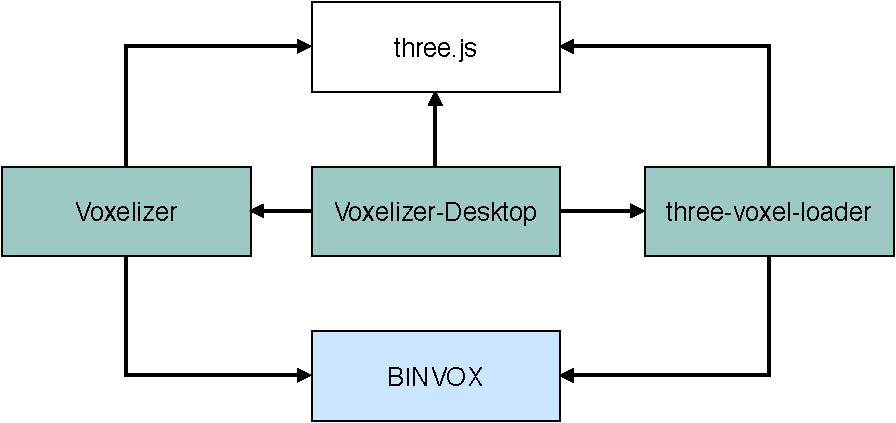
\includegraphics[page=1,scale=1]{sections/introduction/figures/systems-overview.pdf}
    \caption{Automation of release publishing process.}
    \label{fig:systems-overview}
\end{figure}

\subsection{Automation overview}
\colorbox{RubineRed}{Include diagram of simple github automation prosess?}

%%=========================================
\section{Outline}

The rest of the report is structured as follows.\\
\break
\textbf{Chapter 2 - Theory:} Chapter two gives an introduction to the theoretical background .... \\
\break
\textbf{Chapter 3 - Method:} Contains a description of the methodology and materials that were considered throughout the project ....\\
\break
\textbf{Chapter 4 - Result:} Contains a description of the finished software systems \\
\break
\textbf{Chapter 5 - Discussion:} Discusses the achieved results, the execution of methodologies and tools, in addition to encountered difficulties.\\
\break
\textbf{Chapter 6 - Conclusions:} This chapter presents an overall conclusion of the project, reviewing the objectives and the progress made. \\
%This is chapter 2
%%=========================================
\chapter{Theoretical basis}

%%=========================================
\section{Agile methods}
\subsection{Scrum}
Scrum is an agile methodology. 
Background and history of the evolution of scrum......
What is it? How does it work?
s
\begin{figure}[h]
    \centering
    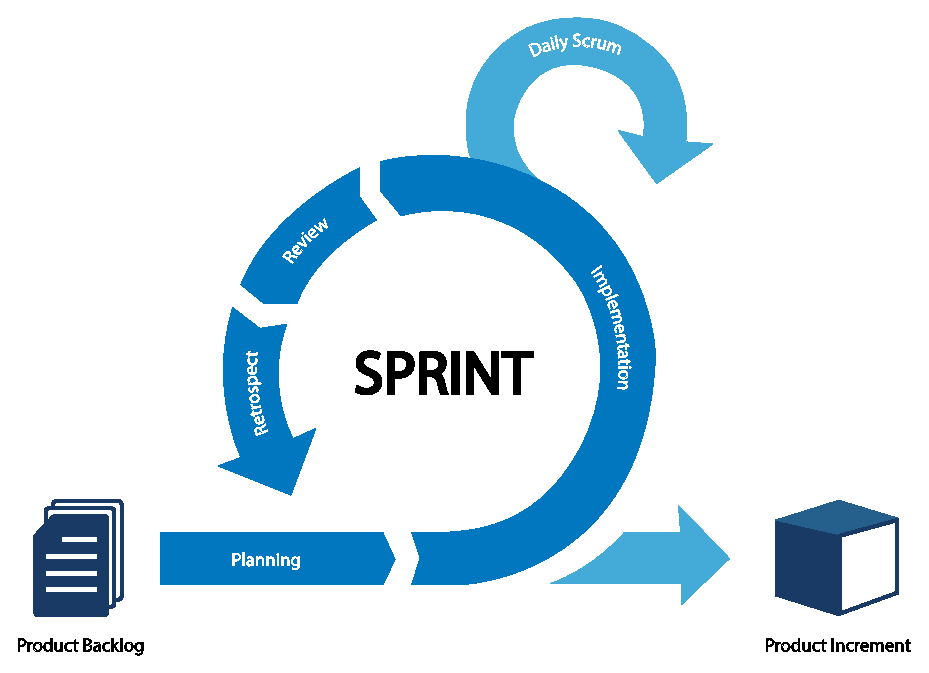
\includegraphics[page=1,width=0.75\textwidth]{sections/theory/figures/scrum.eps}
    \caption{Scrum workflow.}
    \label{fig:scrum}
\end{figure}

\subsection{Kanban}

\section{Git}
Git is a type of distributed version control system (VCS), originally created by Linus Torvalds in 2005. Git is free and opensource, and is today the most popularly used VCS. It is fast and efficient, able to handle everything from small hobby projects to giant projects like the Linux kernel. Every Git directory is a complete repository with history and full version-tracking abilities. It does not need access to internet, nor a central server in order to work.

\subsection{GitFlow}
GitFlow is a popular branching model for Git, created by \cite{gitflow}. Figure \ref{fig:gitflow} displays an example git history, adhering the GitFlow branching style.
\begin{figure}[h]
    \centering
    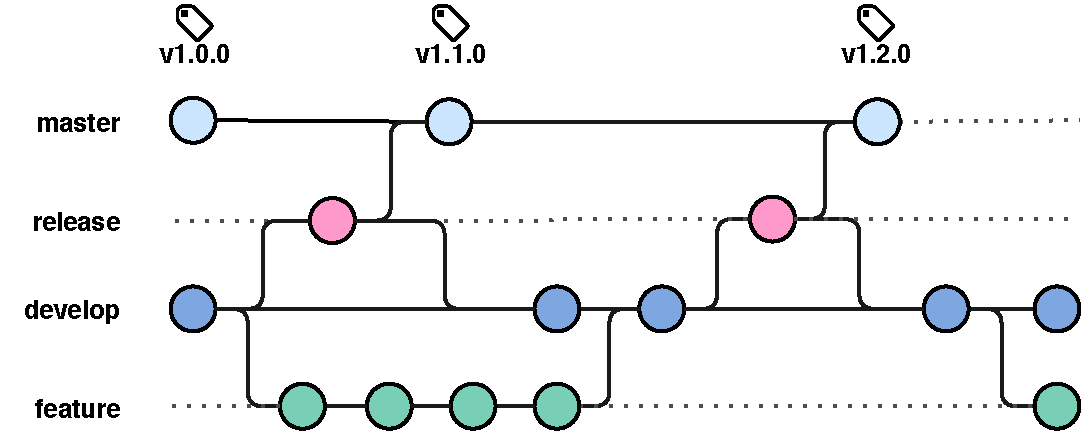
\includegraphics[page=1,width=\textwidth]{sections/methodology/figures/gitflow.pdf}
    \caption{GitFlow branching model example.}
    \label{fig:gitflow}
\end{figure}

\section{GitHub}
GitHub is primarily a hosting service for Git repositories. The company was acquired by Microsoft in 2019. In addition to repository hosting, GitHub provides a range of different services through it's web-based GUI. This includes both wikis, access controls, simple task management tools, automation capabilities and websites hosting.

\subsection{GitHub Actions}
GitHub Actions \cite{github-actions} is a fairly very new service provided by GitHub. It enables users to automate software workflows, effectively providing a high quality CI/CD for free \footnote{GitHub Actions usage is completely free for public repositories. For private repositories, depending on the subscription plan, some thousand minutes of free usage is provided each month.}. It is also possible to set up self-hosted runners. GitHub Actions makes it possible to both build, test and deploy code directly from within GitHub.

\subsection{GitHub Pages}
Github provides its users with a public webpage hosting service. This is named GitHub Pages \cite{github-pages}. User are able to serve static websites directly from their repository hosted on GitHub.

\section{HyperText Markup Language (HTML)}
HTML is a markup language, originally defined by Tim Berners-Lee and Robert Caillau in 1989. It is primarily used for documents on the web, intended to be displayed in a web-browser. It is used for structuring and formatting information. HTML can be used in conjunction with other web technologies such as Cascading Style Sheets (CSS) and scripting languages like JavaScript, in order to either style or dynamically change and alter the contents of a web page. The currently latest release of the language is HTML5.

\section{Cascading Style Sheets (CSS)}
CSS is short for Cascading Style Sheets. CSS is a programming language in order to describe how HTML elements in a HTML file are to be rendered. Everything from the boldness of a headline, to the background of the entire page.

\section{JavaScript}
JavaScript is a lightweight interpreted programming language. The language is prototype-based, a type of object-oriented programming where properties and methods are added to an instance of an implicitly defined class \cite{prototype-based-programming}. JavaScript does not provide any type-checking.

JavaScript was developed by Brendan Eichand and released in 1995 \cite{javascript-original-release}. Initially, it was designed to be a small scripting language for enabling interaction with web pages. A standardization effort of JavaScript, led by Ecma International \cite{ecma-international}, lead to the ECMAScript specification.  that the modern JavaScript language conforms to. Several releases. Since then, the language has evolved rapidly and gained massive in popularity. It has become the de-facto language for adding dynamic behavior to HTML. As of may 2020, JavaScript is among the top ten programming languages according to the TIOBE index \cite{tiobe-index}.

% Node.js
Originally, JavaScript engines were mainly used in browser environments. However, with the development of Node.js in early 2009, this was dramatically changed. Node.js provides a runtime environment for executing JavaScript outside of a web browser. It set the stage for server-side JavaScript programs. In January 2010, a package manager named npm \cite{npm} was released for Node.js. This made it easy for developers to share and use source code.

% Module bundlers
The size of JavaScript programs has increased massively in size. With increased size, so does the complexity of the code. However, JavaScript had very limited functionality in terms of splitting a program up in smaller modules for use with the browser. Maintaining large codebases was a nightmare. It therefore became apparent that a way of breaking down a JavaScript program into smaller modules was needed. Several open-source module systems were therefore developed by the community in order to tackle this problem.

\subsection{Module systems}
\begin{itemize}
    \item \textbf{CommonJS} is a module specification meant for JavaScript outside the browser. It is mainly used in Node.js, and hence it is one of the most popularly used module definitions. The modules are mainly imported and exported with the keywords "require" and "module.exports".
    \item \textbf{Asynchronous module definition}, or more commonly known as AMD, is a JavaScript module definition intended for the browser. It defines an API for defining code as modules, including their dependencies. AMD also has the capability of loading modules asynchronously. The most popular AMD module loader is named RequireJS \cite{requirejs}.
    \item \textbf{Universal Module Definition}, abbreviated UMD, is a module definition wrapper to be able to use various module systems \cite{universal-module-definition}. Be it in the browser or in Node.js. It is compatible with both CommonJS and AMD.
    \item \textbf{JavaScript modules}, or ES Modules, are a language native module system, introduced with ECMAScript 2015 (ES6) in 2015. The implementation is relatively new, so a lot of libraries, frameworks and packages does not support this yet. Still, most browsers have already implemented support for this \cite{es-modules-support}.
\end{itemize}

\subsection{Transpilation}
\label{sec:intro-transpilation}
Due to the many versions of JavaScript, or more specifically ECMAScript, like ES5, ES6 and ES7, compatibility is an issue. Not all browsers and environments support the latest ECMAScript versions. Tools like Babel \cite{babel} has been developed in order to transpile JavaScript to a specific version. The most common transpilation target, supported by all the major browsers is ECMAScript 5 (ES5).

\subsection{Bundling}
\label{sec:intro-bundling}
JavaScript bundling is an optimization technique to combine separate resource files into one file. This is done in order to reduce the number of HTTP requests required for a page to load. Several bundlers are able to do so called tree-shaking, dramatically reducing the size of the finished bundle. In addition to the performance gain, bundling is also often done in order to develop a JavaScript application in separate files, effectively employing a form of module system. The bundlers often use one or more of the popular module systems like UMD and ES modules. There are three main actors in terms of bundling JavaScript.
\begin{itemize}
    \item \textbf{Webpack} \cite{webpack} is a module bundler for JavaScript. However, id is also able to transform front-end assets like HTML, CSS, and images. Webpack is mostly used for bundling JS applications, and is highly extendible. It also provides a way to bundle an application for Node.js to be used in the Browser \footnote{This requires that no Node.js specific APIs are used. Alternatively, polyfills could be supplied.}. However, as of may 2020, it does not support exporting ES Modules.
    \item \textbf{Rollup} \cite{rollup} is a module bundler primarily focusing on JavaScript libraries. It has a lot of similarities with Webpack. However, it is a bit lighter and provides exporting support for ES Modules.
    \item \textbf{Browserify} \cite{browserify} is a lightweight module bundler for enabling the use of CommonJS syntax in the Browser.
\end{itemize}

\section{TypeScript}
TypeScript \cite{typescript} is a typed superset of JavaScript that compiles to plain JavaScript. It is open source, and primarily developed and maintained by Microsoft \cite{microsoft}. TypeScript provides optional static typing to the JavaScript language. The TypeScript compile also includes support for the latest ECMAScript features.

\section{JavaScript Object Notation (JSON)}
JavaScript Object Notation, better known as JSON, is a lightweight data interchange format. It is easy for both humans and machines to read and write. The data is stored as attribute–value pairs. An example is shown in Program Code \ref{lst:json-example}.
\lstinputlisting[language=JSON,style=numbers,caption={Example JSON data},label={lst:json-example}]{sections/theory/code/json-example.json}

\section{JSDoc}
JSDoc is markup language for annotating JavaScript source code files. The JSDoc specification was released in 1999. Today it has become the de-facto JavaScript documentation language. It is for example used in projects like the Google Closure Compiler \cite{google-closure-compiler} by Google. Since JavaScript has no type-checking, JSDoc is able to patch some of this inconvenience. By using various tools, one is able to generate documentation in formats like HTML and RTF. JSDoc 3 is the current version of the original companion documentation generation tool for JSDoc. JSDoc 3 \cite{jsdoc-3}, also referred to as just JSDoc, is the most used tool for programmatically generating JavaScript documentation. It has a wast feature set, even allowing users to create customized themes, known as templates. Currently, JSDoc is used by more than 38.800 public projects \cite{jsdoc-used-by}, and has over 10.600 stars on GitHub \cite{jsdoc-stargazers}.

\section{Tools and libraries}
\subsection{ndarray}
ndarray is an open-source JavaScript package providing modular multidimensional arrays, written by Mikola Lysenko in 2013. In short does ndarray implement a higher dimensional views of 1D arrays. The 1D array can either be a normal JavaScript  Array, or a JavaScript typed array. MDN defines typed arrays as \textquote[\citet{mdn-typed-arrays}]{array-like objects that provide a mechanism for reading and writing raw binary data in memory buffers.}. Mainly, they are used for maximizing efficiency and reducing memory footprint. However, typed arrays are normally quite difficult to work with in JavaScript. Multidimentional typed arrays even more so. ndarray provides a simple but powerful API, making use of multidimensional typed arrays easy.

\subsection{Electron}
Electron \cite{electron} is an open-source framework developed and maintained by \citet{github}. It allows one to build cross-platform desktop applications with JavaScript, HTML and CSS. Electron is used by thousands of people, and apps like Visual Studio Code \cite{visual-studio-code}, Facebook Messenger \cite{messenger} and Microsoft Teams \cite{teams} are all made with Electron.

\subsection{React}
React \cite{react} is a JavaScript library for building user interfaces, created by \citet{facebook}. It is based around components, where each component manage its own state. These are then composed together, enabling the creation of intricate and complex UIs. The library also implements its own syntax extension to JavaScript. It is named JavaScript XML, or the more popular used term - JSX. In addition to this, there exists a vast ecosystem of plugins for React, greatly simplifying the implementation of everything from localization to state management.

\subsection{Semmle LGTM}
LGTM by Semmle \cite{lgtm} is a web service providing code security analysis. The service is free for open-source projects. LGTM integrates with GitHub and Bitbucket, and is able to analyze projects written in Java, Python, JavaScript, TypeScript, C\#, Go, C and C++. It seeks out to combat the manual process of finding vulnerabilities. By catching them at an early stage, one can prevent vulnerabilities from reaching production. LGTM is based on large community of top security researchers, making it possible to help developers ship secure code \cite{lgtm-security}.

\subsection{Coveralls}
Coveralls \cite{coveralls} is a web service for code testing coverage. It enables one to track a projects code coverage over time, providing valuable insight in a projects testing suite. Coveralls also features close integration with GitHub, enabling pull request coverage reviews.

\section{Data structures}
\subsection{Octrees}

\subsection{Bounding volume hierarchy }
A bounding volume hierarchy, abbreviated BVH, is a type of tree structure.

\section{3D computer graphics}
3D computer graphics refers to three-dimensional representation of geometric data in computers, normally to be rendered to a two-dimensional image. The finalized render may be saved or displayed on a screen in realtime. The geometric data is usually a 3D model, stored in an appropriate file format. The most basic polygon primitives in computer graphics includes vertices, edges and faces. A vertex is simply point in space. An edge is a connection between two vertices. A face is a closed set of edges. Figure \ref{fig:triangular-mesh} shows a yellow triangle with the appropriate vertex, edge and face labels. These primitives together defines a polyhedral. Polyhedrons can then be further grouped together into a mesh. The most common type of polygon mesh is a triangular mesh. This is a mesh comprised of only triangles. Figure \ref{fig:triangular-mesh} shows an illustration of a section of a triangular mesh.
\begin{figure}[h]
    \centering
    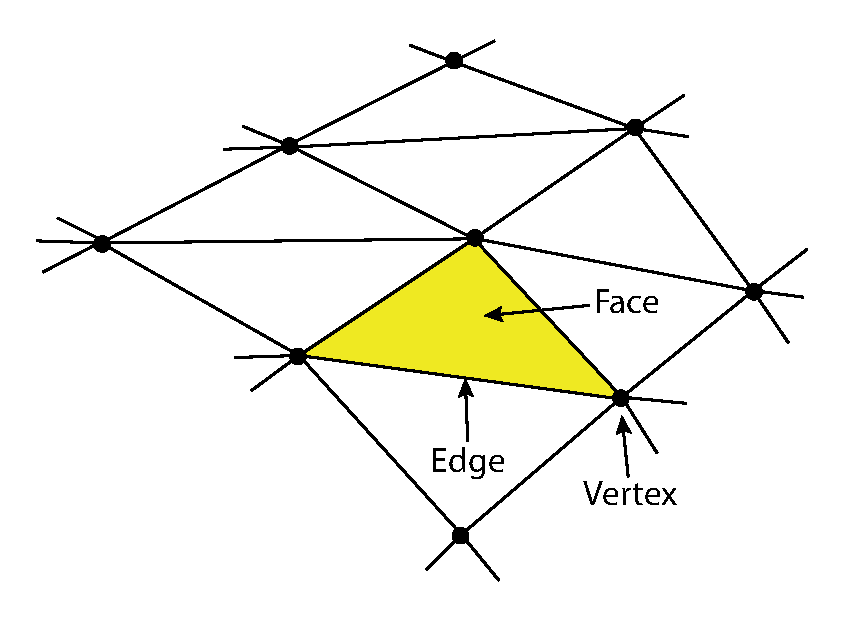
\includegraphics[width=0.75\textwidth]{sections/theory/figures/mesh.eps}
    \caption{Triangular mesh}
    \label{fig:triangular-mesh}
\end{figure}

\subsection{Texture maps}
A texture map is an image which is applied, or mapped, onto the surface of a geometry. The images is often in the form of a bitmap image or a procedural texture. Texture mapping, or UV mapping, is the process of projecting an actual 2D image onto a 3D model. The technique was initially developed by Edwin Catmull in 1974 \cite{catmull-texture-mapping}. UVs are two-dimensional texture coordinates, assigned to every vertex in a polygon. They are essential in terms of describing how an image gets applied onto a geometry. Figure \ref{fig:texture-mapping} shows an illustrative example of how a 2D image gets "wrapped" around a 3D model. A lot of 3D modeling software are able to do the UV unwrapping automatically, for example Blender \cite{blender}. It is also possible to map a finalized render into a surface texture, a process known as baking \cite{blender-texture-baking}. This is primarily used as an optimization technique.

\begin{figure}[h]
    \centering
    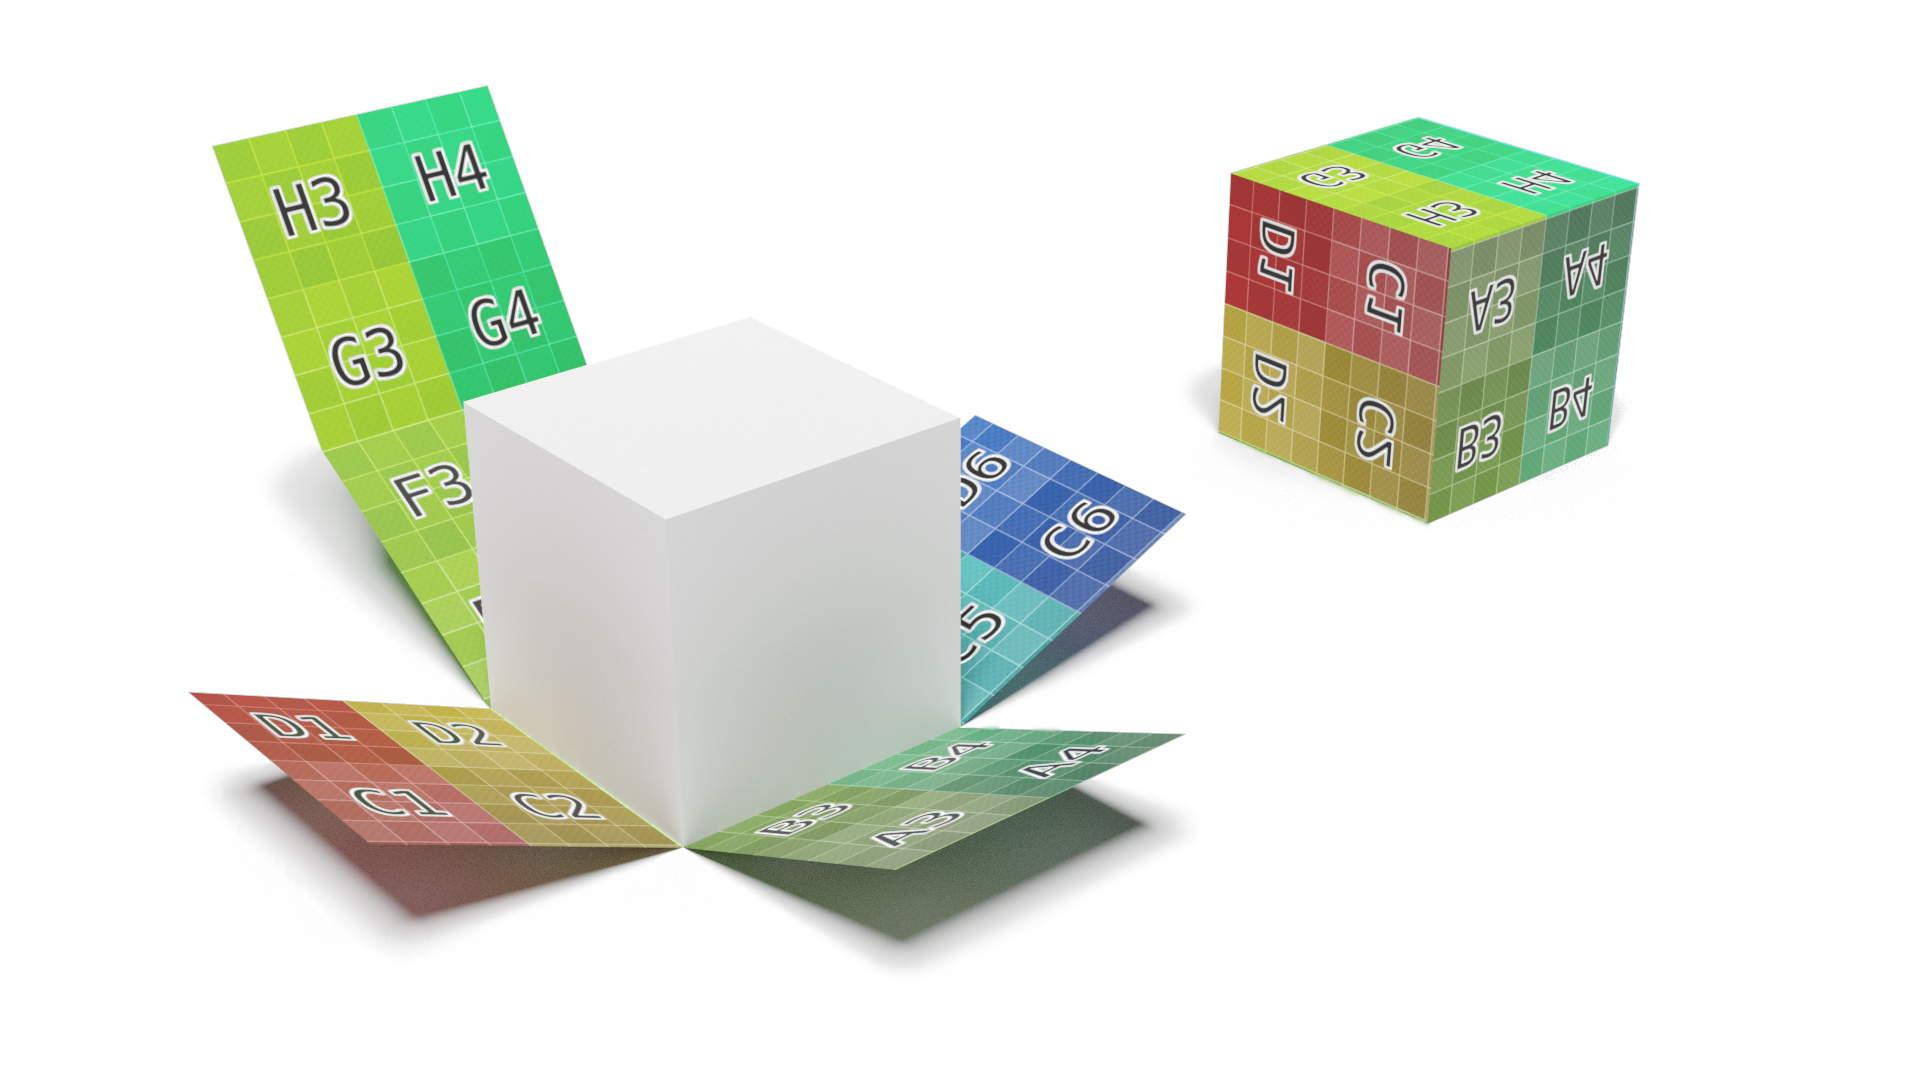
\includegraphics[width=\textwidth]{sections/theory/figures/texture-mapping.png}
    \caption{Texture mapping illustration.}
    \label{fig:texture-mapping}
\end{figure}

\subsection{Ray casting}
Ray casting is the concept of use of ray–surface intersection tests to solve a variety of problems in 3D computer graphics and computational geometry. 
The first use of the term ray casting was made by Scott Roth, in a paper from 1982 titled "Ray casting for modeling solids" \cite{roth-ray-casting}. Raycasting is demonstrated in Figure \ref{fig:raycasting-intersections-example}. A ray is directed towards an object. If it crosses a face, an intersection is registered.

\begin{figure}[h]
    \centering
    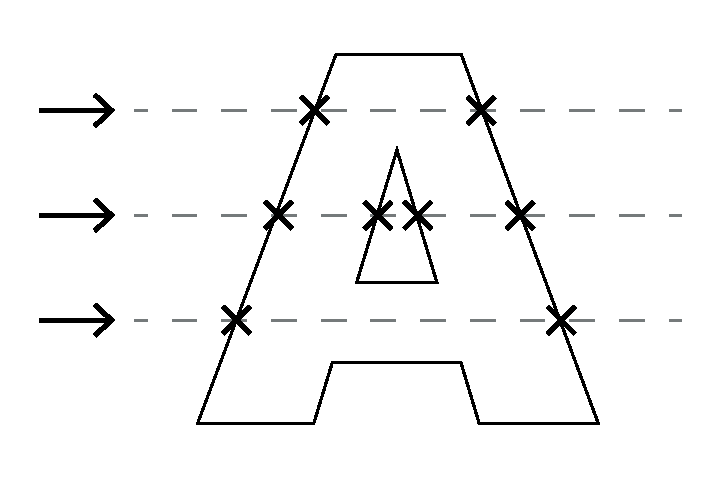
\includegraphics[scale=0.8]{sections/theory/figures/raycast-intersections}
    \caption{Raycasting intersections example.}
    \label{fig:raycasting-intersections-example}
\end{figure}

\subsection{OpenGL}

\subsection{WebGL}
Uses OpenGl ES, a subset of OpenGL. ...

\subsection{three.js}
three.js abstracts away a lot of the manual handling of constructing vertices, faces, setup of WebGL ....

\section{Voxel}
A voxel is the three-dimensional analogue of a pixel \cite{wiki-voxel}. It represents a single data point in a regularly spaced three-dimensional grid. Figure \ref{fig:three-voxels} shows an illustration of three voxels, where one of the voxels are marked with blue color. A very common use of voxels are in medical imaging, for example datasets produced by a CT scan. Other areas where voxels are commonly used includes simulations and for representing terrain in games.

\begin{figure}[h]
    \centering
    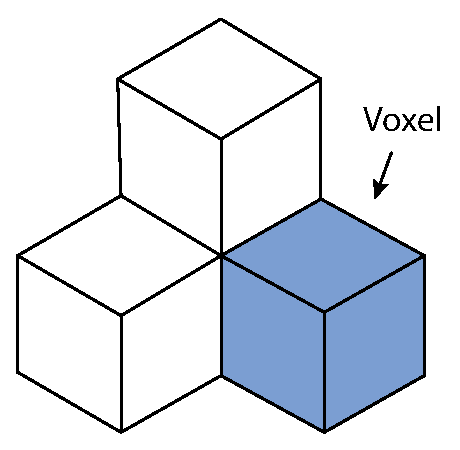
\includegraphics[width=0.4\textwidth]{sections/theory/figures/voxels.eps}
    \caption{Three voxels.}
    \label{fig:three-voxels}
\end{figure}

\section{Voxelizer v0.1.3}
Voxelizer v0.1.3 \cite{voxelizer-v0.1.3} is a JavaScript library for conducting voxelization of 3D models. It was written by me, André Storhaug, in 2019. Version 0.1.3 features a relatively simple voxelization algorithm which is based on raycasting. The sampling algorithm tries to produce a filled volume-representation of a supplied 3D model. It samples the front and the back of the model, combines the two results together and tries to fill the in-between gap. The 3D model loading capabilities of the program is limited to plain OBJ files. In terms of exporting, the software is able to output a 3D JavaScript array (nested arrays).

The library is using ES6 features, hence it is transpiled with Babel (see Section \ref{sec:intro-transpilation}). However, the library is not bundled. It is therefore not possible to use the program out of the box in a browser. One is limited to Node.js, or setting up a build system involving a module bundler like Webpack or Rollup, as described in Section \ref{sec:intro-bundling}. The source code is messy, and it is very hard to extend functionality. Especially due to a severe lack of documentation.

Voxelizer v0.1.3 produces unsatisfactory voxelization results. Firstly, several of the voxelizations contains holes. This can be clearly seen in Figure \ref{fig:voxelizer-v0.1.3-torus}. A voxelization with holes often renders the voxelization useless. Secondly, a lot of artifacts are often generated, severely degrading the results. This is shown in Figure \ref{fig:voxelizer-v0.1.3-monkey}, where long strains of voxels appear in the front of the model. Thirdly, the software is only able to produce a filled voxelization result. Shell voxelization is therefore not an option.

\begin{figure}[h]
    \centering
    \begin{subfigure}[b]{0.49\textwidth}
        \centering
        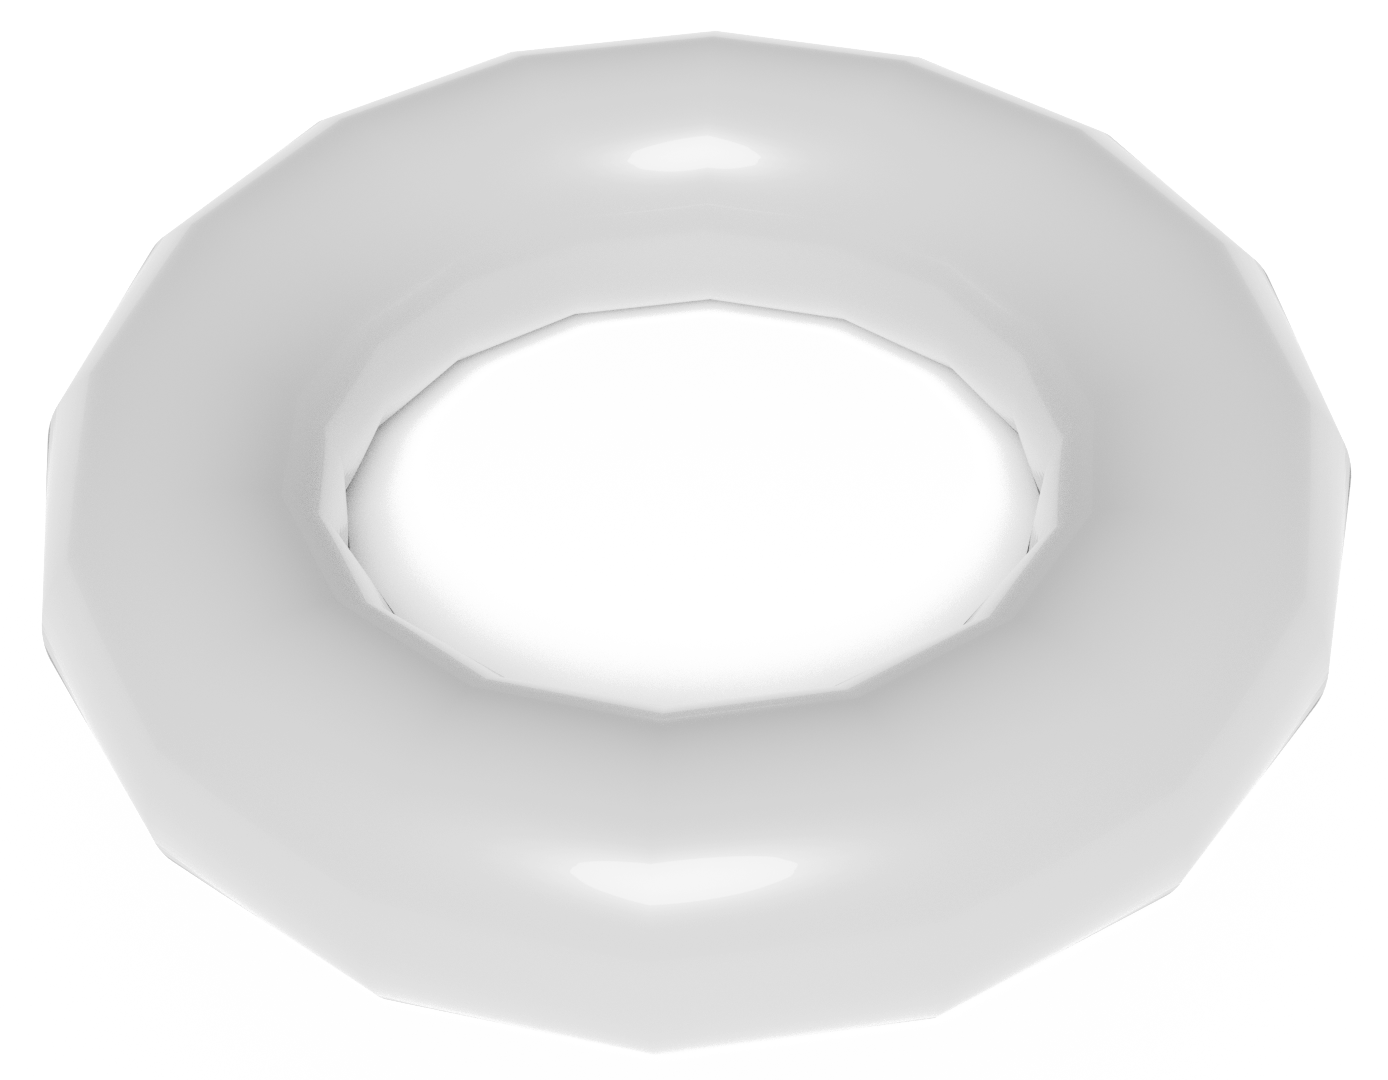
\includegraphics[width=\textwidth]{sections/theory/figures/torus.png}
        \caption{Original torus mesh.}
        \label{fig:original-torus}
    \end{subfigure}
    \hfill
    \begin{subfigure}[b]{0.49\textwidth}
        \centering
        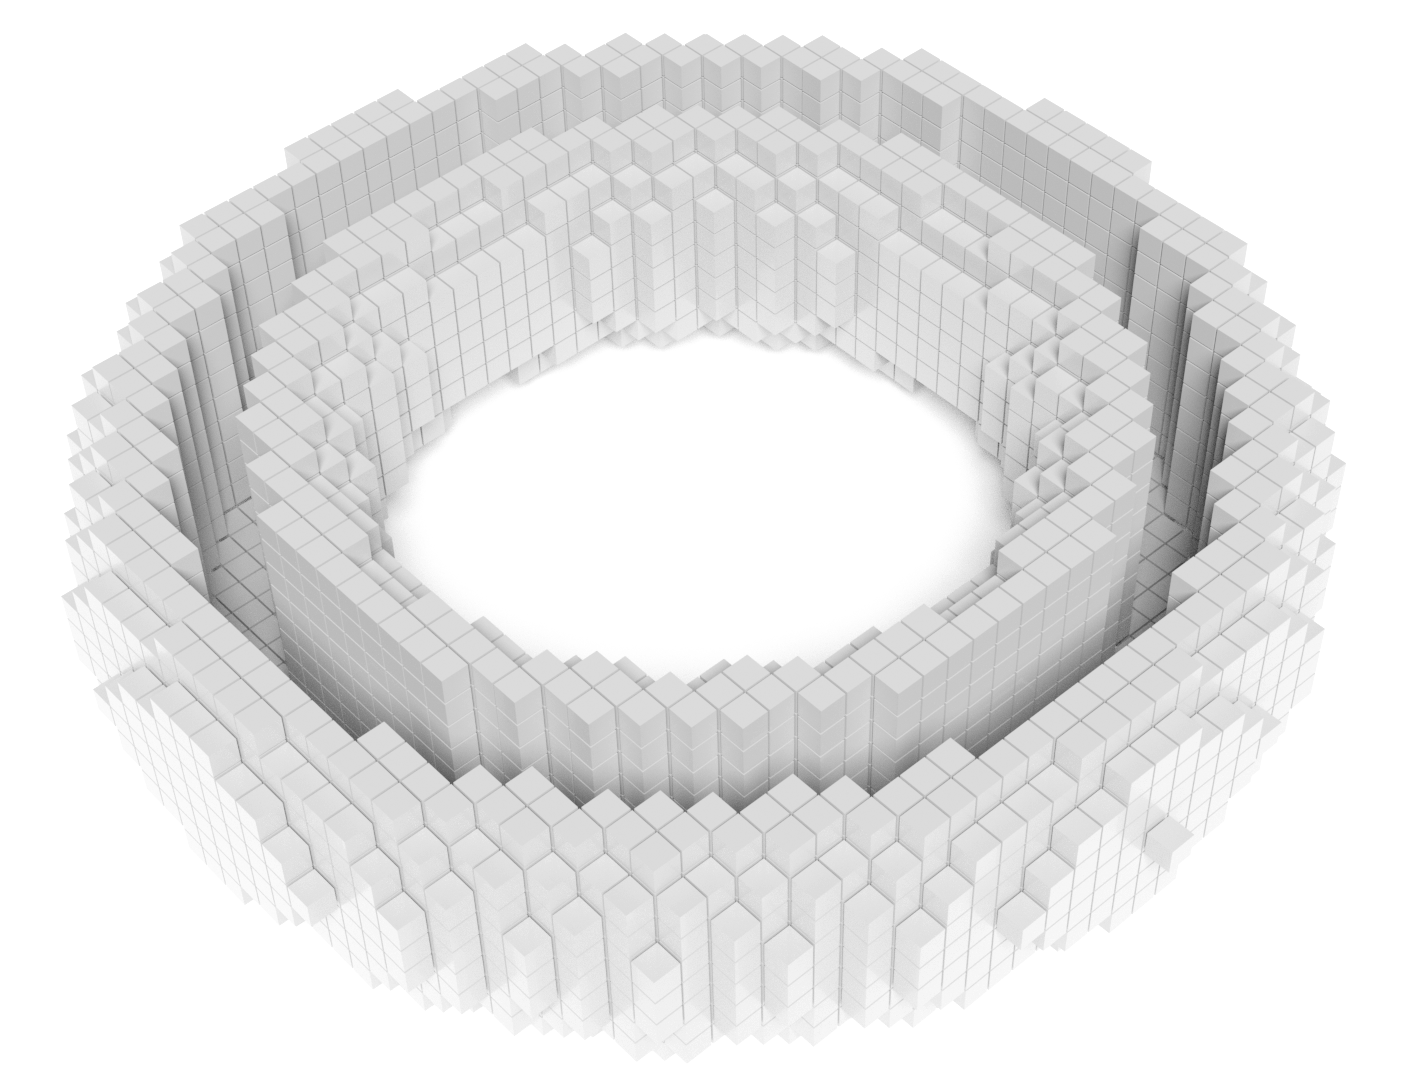
\includegraphics[width=\textwidth]{sections/theory/figures/voxelizer-v013-torus-40.png}
        \caption{Voxelized result.}
        \label{fig:voxelizer-v0.1.3-torus}
    \end{subfigure}
    \caption{Voxelization of a torus with Voxelizer v0.1.3. Resolution of 40.}
    \label{fig:voxelizer-v0.1.3-torus}
\end{figure}

\begin{figure}[h]
    \centering
    \begin{subfigure}[b]{0.46\textwidth}
        \centering
        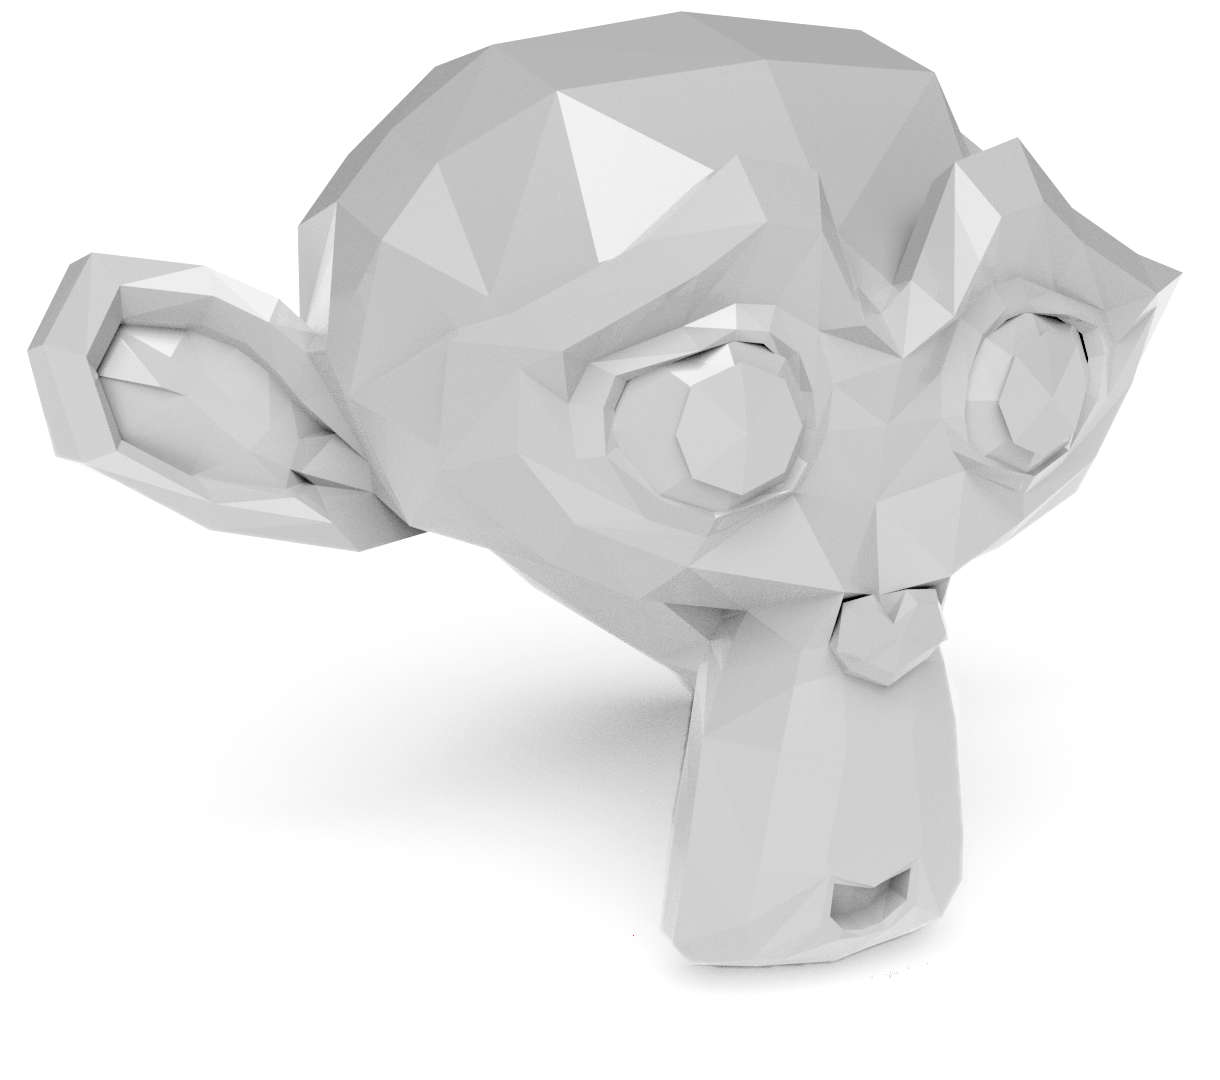
\includegraphics[width=\textwidth]{sections/theory/figures/monkey.png}
        \caption{Original monkey mesh.}
        \label{fig:original-monkey}
    \end{subfigure}
    \hfill
    \begin{subfigure}[b]{0.53\textwidth}
        \centering
        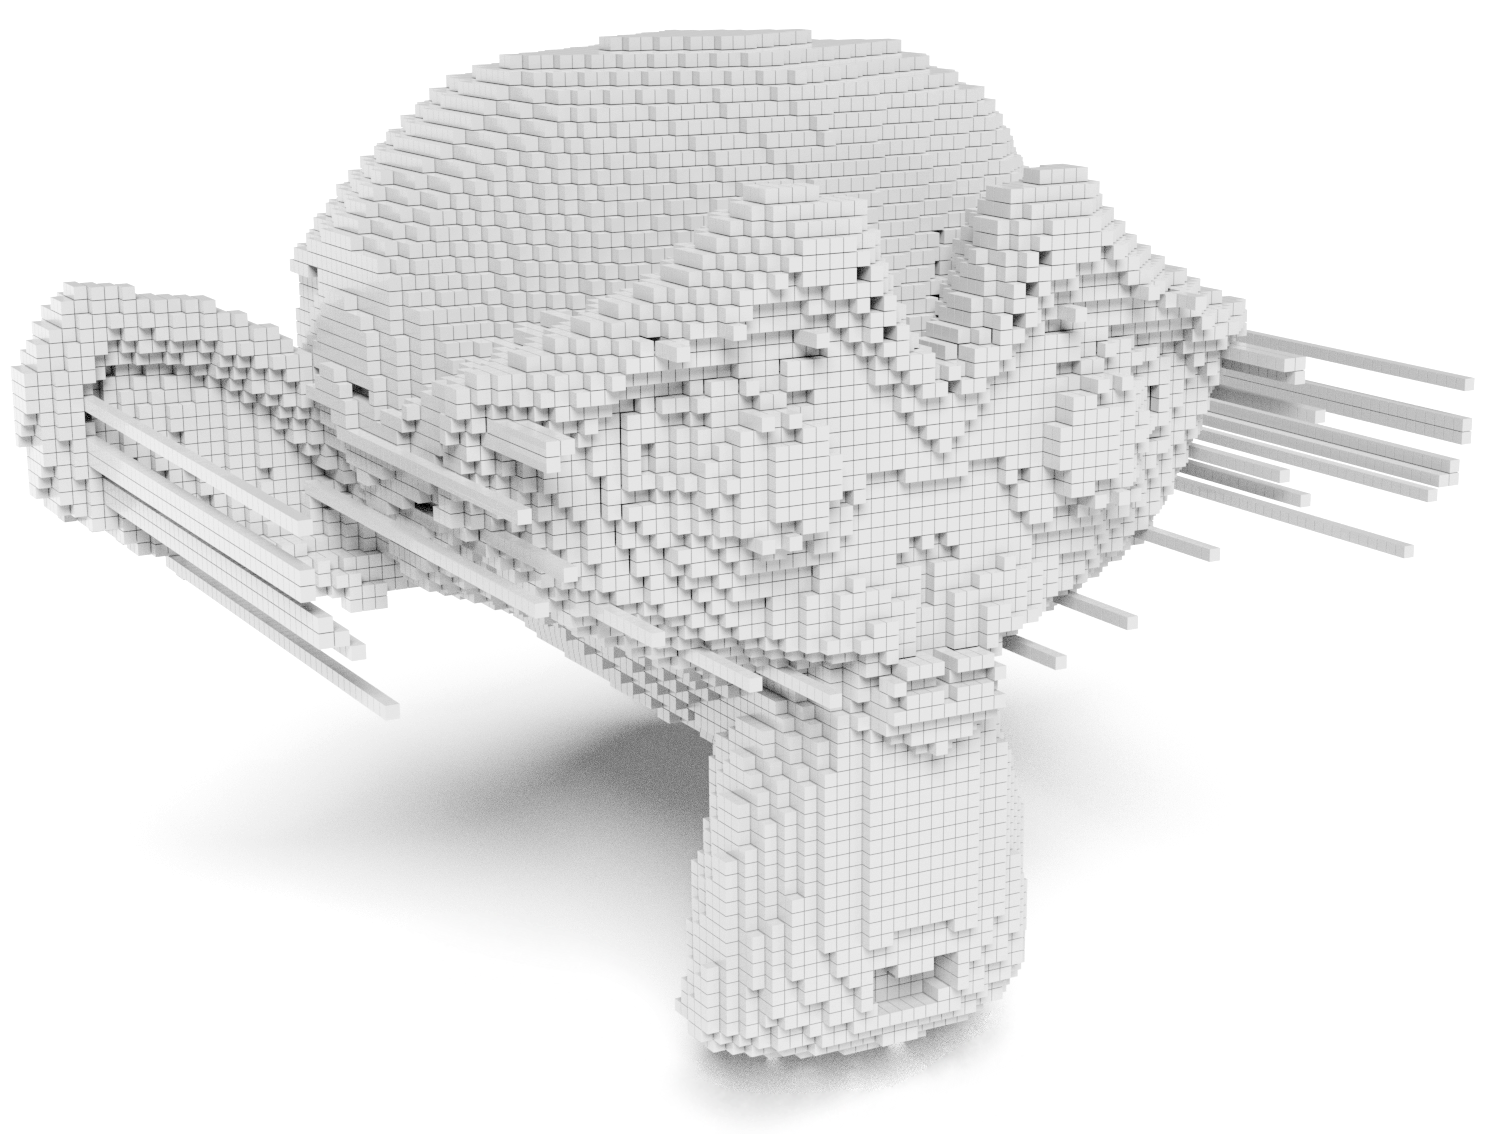
\includegraphics[width=\textwidth]{sections/theory/figures/voxelizer-v013-monkey-100.png}
        \caption{Voxelized result.}
        \label{fig:voxelizer-v0.1.3-monkey}
    \end{subfigure}
    \caption{Voxelization of a monkey with Voxelizer v0.1.3. Resolution of 100.}
    \label{fig:voxelizer-v0.1.3-monkey}
\end{figure}

%This is chapter 3
%%=========================================
\chapter[Method]{Materials and methods}

%In this final chapter you should sum up what you have done and which results you have got. You should also discuss your findings, and give recommendations for further work.

%%=========================================

\section{Tools and libraries}
\subsection{JavaScript}
JavaScript has mainly been chosen as the base implementation language because of its cross compatibility and popularity. ...

\subsection{Babel}
- Babel - ES6 needs to be transpiled to ES5 (Browser compatibility).
\subsection{npm}
Needed packages.. Published all packages to npm.. Most stabile compared to GitHubs new repo....

\subsection{Third party libraries}
Why did i use them???
list up like:
- xxx because ...
- xxx provides ...
Elaborate some on three.js - why is it good? (popularity)

\subsection{GitHub Actions}
Why? How did i use it? - For automation... - deeply integrated in GitHub.

\section{Working methodology}
\subsection{Scrum}
Even though this is a one man project, i have tried to adapt the scrum methodology.
...

\subsection{Requirements specification}
\subsubsection{Acceptance criteria}
Acceptance criteria - custom field in Jira.
Specially for the voxelization algorithm?

\subsection{GitFlow}
Why did i follow gitflow? Any changes to the usage?? Good for enforcing standards, automation etc..

\subsection{Semantic versioning}
All published modules are enforcing Semantic versioning. This ....

\section{three-voxel-loader}
\colorbox{green}{NEED UML DIAGRAMS}\\
The main goal for the three-voxel-loader is to generate a 3D mesh based on voxel data. The next subsections will present a walkthrough of how the plugin is implemented, including the various design choices made.

\subsection{Internal data structure}
For the plugin to be able support loading of various voxel data formats, an internal data structure is used. This serves as an interface for the processing of various voxel data internally in the plugin. The chosen data structure is an octree, as described in Section~\ref{sec:theory-octree}. The actual implementation of the octree is done with the sparse-octree library by Raoul van R\"uschen~\cite{sparse-octree}. There are several reasons behind the choice of using an octree. 

Voxel data normally consists of very large amounts of data. One of the main limitations for how big a dataset can be, is the amount of available computer memory (RAM). The memory footprint of the plugin is therefore a big concern, especially since the targeted runtime environments are often placing further restrictions on the available memory resources. Voxel data normally contains very large amounts of empty space, or "air". This data is not needed for generating the polygon mesh. Only the data about the actual voxels and their locations are of interest. The location of the voxels are normally not stored explicitly, but rather derived by their relative location to neighboring voxel cells. An octree is especially well suited for this purpose. Since an octree is based on partitioning of space, large amounts of this empty space in the voxel data can be discarded. This works especially well if the voxel data is clustered.

Octrees also makes it easy to implement a Level of Detail (LOD) mechanism. By determining the desired depth of the octree, one are able to simplify the detail of the voxel data. This is very valuable, as generating mesh geometry for every voxel is placing high stress on the available hardware resources. Being able to control the LOD, this can be very effective in terms of simplifying the resulting mesh.

\subsection{Loading voxel data}
In order to actually load the voxel data (by generating an octree), several loader classes have been created. These classes all extend the \textit{loader} class defined in three.js, providing both consistency and tight integration with library. It also ensures that extending the support for more file loaders in the future is easy. Finally, a factory pattern has been implemented for getting and instantiating the desired voxel loader. This makes it able to define an easy-to-use API, where the user only needs to supply the actual voxel data and the corresponding format.

The currently implemented loaders supports several file formats, including XML, VOX and BINVOX. It is also possible to import plain 3D arrays. Several of the loaders also supports color of the voxels. Following is a brief description of these loaders.
\begin{itemize}
    \item \textbf{XML} - XML is an incredible versatile file format. For implementing the XML loading, the native JavaScript DOM parser is used for the actual parsing of the XML data. The format supports color data. The required format of the XML document structure is described on the GitHub wiki page for the plugin. \colorbox{red}{PROVIDE LINK HERE!!!!!}
    \item \textbf{VOX} - VOX files are loaded with a third party package named \textit{format-vox}~\cite{format-vox}. The VOX file format is provided by MagicaVoxel, a popular voxel graphics editor. VOX files supports color data.
    \item \textbf{BINVOX} - BINVOX \cite{binvox-file-format} is one of the more popular voxel data file formats. BINVOX is the file format used by the binvox~\cite{binvox} voxelization software. A separate repository named binvox~\cite{andstor-binvox} has been created for handling BINVOX files. See Section \ref{sec:method-binvox}
    \item \textbf{3D array} - The 3D array loader is implemented by simply iterating the multidimensional array. For loading color data, a 4D array with RGB values has to be supplied along the 3D array.
\end{itemize}

\subsection{Visualization}
The most intuitive way to visualize a voxel is in the form of a cube. BoxBufferGeometry from three.js has therefore been used to generate the individual 3D visualization of the voxels. However, one BoxBuffer geometry consists of no less than twelve triangles. The number of triangles generated for visualizing the mesh is therefore twelve times the number of voxels. One of the more time consuming operations in terms of actually displaying the 3D graphics, is the number of draw calls made to the graphics API. In order to limit this, all the generated box meshes are merged into one big mesh. For actually coloring the voxels, color is applied to the vertices of the generated box meshes.

\subsection{Debugging}
For actually developing and testing the plugin, a HTML page was created. The page includes basic setup of three.js, alongside various input controls for inspecting and testing the three-voxel-loader plugin. The input controls are provided by a lightweight JavaScript controller library named dat.gui~\cite{dat.gui}. In the end, the debugging solution were polished and deployed to GitHub Pages, serving as an example for the various functionality the plugin provides. \colorbox{red}{LINK TO GITHUB PAGES EXAMPLE}

\subsection{Building}
The plugin is bundled with Rollup. This produces excellent bundles, with support for both UMD and ES Modules. See Section~\ref{sec:theory-bundling} for more details on Rollup, and Section~\ref{sec:theory-module-system} for UMD and ES Modules. three-voxel-loader makes use of ES6 features. All source files are therefore transpiled to ES5 with babel.

\section{Voxelizer}
Short intro
Three.js provides raycasting out  of the box. However, the raycasting method implemented It would be more efficient to implement the raycasting directly without the use of three.js. However, this would be laboursome. However, the main reason for using the three.js library is based on the popularity of the project. the ecosystem of three.js is vast, providing everything from file loaders to ... This, combined with excellent documentation, should make it very easy to produce a 3D model in three.js. This sets the stage for further processing of the 3D models with the Voxelizer engine.

\subsection{Implementation}
\label{sec:method-implementation}
\colorbox{RubineRed}{UML diagram of system here}

The system is broken down in several modules (folders). This includes:
\begin{itemize}
    \item \textbf{core} - The core module contains core APIs. This provides the main user API for conducting the voxelization.
    \item \textbf{algorithms} - The algorithm module defines the algorithm system. This is in charge for the actual sampling of the 3D models.
    \item \textbf{color} - The coloring system is found in the color module. This manages the color extraction for supporting color voxelization.
    \item \textbf{volume} - The volume module mainly contains a wrapper class for providing a consistent interface for interacting with volumes throughout the application.  
    \item \textbf{exporters} - The exporters module is made up of various exporter classes. These enables the engine to export the voxel data into many different formats.
    \item \textbf{utils} - This module contains various utility functions.
\end{itemize}

\subsection{Algorithm system}
Voxelizer implements an algorithm system that makes it easy to extend the voxelization support. Be it new algorithm types or options. The system mainly consists of two base abstract algorithm classes. One for plain voxelization, and one which is colorable. By simply extending the appropriate base class, a new algorithm can be defined. Further, a factory pattern has been implemented for selecting the appropriate algorithm.

Since the generated voxel data can be huge, an efficient internal data structure needs to be used. Here is two main concerns to take into account. The first is the memory footprint. In order to be able to do high resolution voxelizations, a limiting factor is the amount of available system memory. A second and bigger concern is speed. The JavaScript engines are able to do quite a lot of optimization. By using the JavaScript language in clever ways, quite high processing speeds can be achieved.

The old Voxelizer v0.1.3 used normal JavaScript arrays which was nested. These arrays grows and shrink dynamically, potentially resulting in slow performance. Although, the JavaScript engines are often able to optimize the execution quite a bit, resulting in decent speeds. However, in order to comply with both the memory and performance requirements, typed arrays have been used instead. More specifically, only one large one-dimensional typed array is used. This is a more low level data type than normal arrays, providing mechanism for reading and writing raw binary data in memory buffers. In order to support multidimensionality, the efficient third party library ndarray is used. See Section \ref{sec:theory-ndarray} for more details on ndarray.

\subsection{Raycasting algorithm}
\label{sec:method-raycasting-algorithm}
The new and upgraded voxelization algorithm is mainly based on raycasting (see Section \ref{sec:theory-raycasting}). Following is a description of how the algorithm works.

First, several preparations are made on the mesh. Firstly, the mesh is centered at the origin. Then the mesh is manipulated to include both front and back faces. This ensures that raycasting against the mesh will result in a hit against both front and back sides of the model. This means that it is not needed to raycast from all 6 sides of the mesh. Hence, the algorithm samples the mesh from the front, left and top sides. These results are then merged together, and returned to the user in form of an ndarray. Figure \ref{fig:voxel-sample-merging} illustrates how these three results are merged, resulting in a complete surface shell representation.
\begin{figure}[h]
    \centering
    \begin{subfigure}[t]{0.3\textwidth}
        \centering
        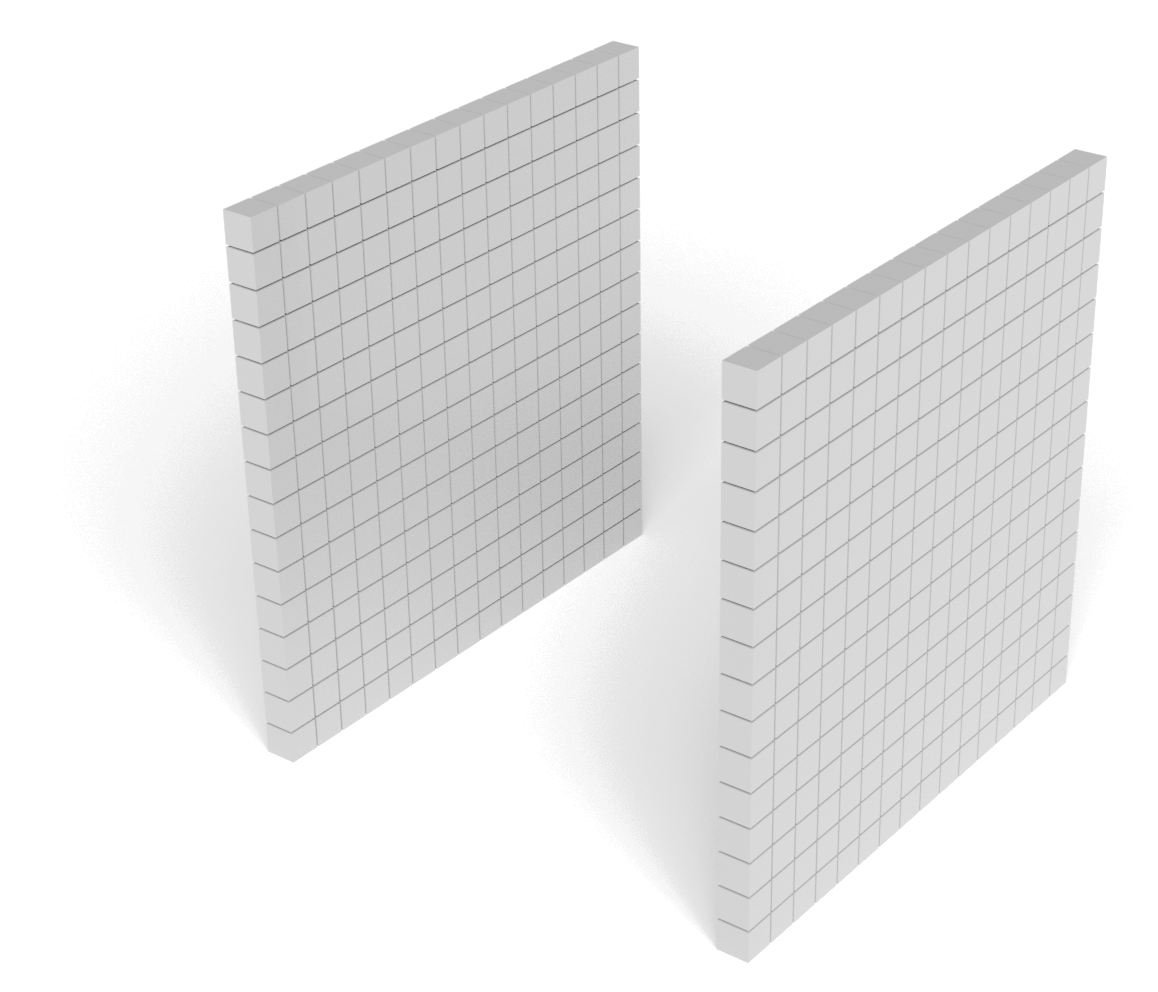
\includegraphics[width=\textwidth]{sections/methodology/figures/voxels-merge-1.png}
        \caption{Front side sample.}
        \label{fig:filling-non-watertight-model}
    \end{subfigure}
    \hfill
    \begin{subfigure}[t]{0.3\textwidth}
        \centering
        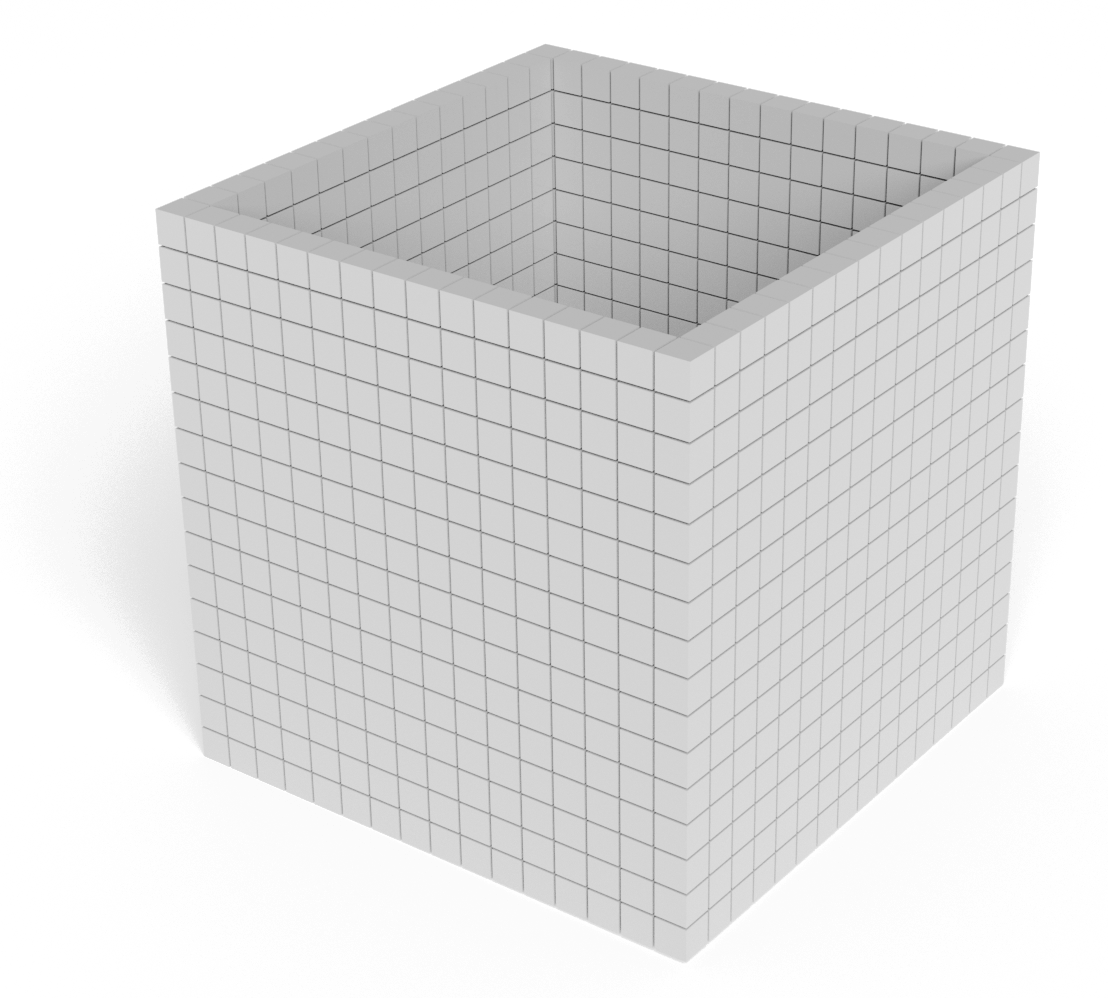
\includegraphics[width=\textwidth]{sections/methodology/figures/voxels-merge-2.png}
        \caption{Front and left side samples merged together.}
        \label{fig:filling-watertight-model}
    \end{subfigure}
    \hfill
    \begin{subfigure}[t]{0.3\textwidth}
        \centering
        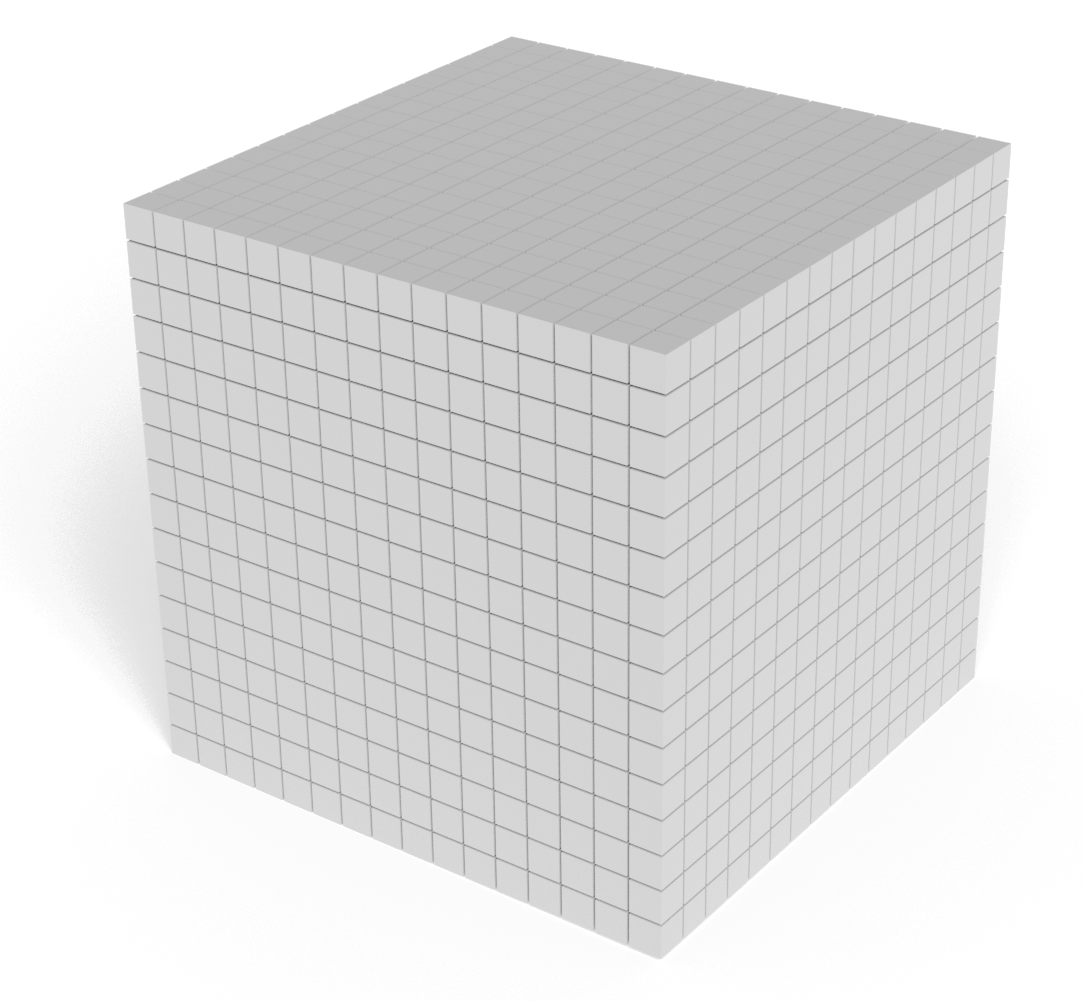
\includegraphics[width=\textwidth]{sections/methodology/figures/voxels-merge-3.png}
        \caption{Front, left and top side samples merged together.}
        \label{fig:filling-watertight-model}
    \end{subfigure}
       \caption{Merging of voxel samplings.}
       \label{fig:voxel-sample-merging}
\end{figure}

The algorithm also has an option for producing filled, or solid, results. This is achieved by interpreting the first raycast intersect as the surface of the object. From this point will everything be considered "inside" the object. When a second intersect is detected, the state is changed to be "outside" the object. A new hit would indicate "inside", and so on. This works very well with a watertight 3D model, as can be seen from figure \ref{fig:filling-non-watertight-model}. However, when trying to fill an object which is not watertight, this can result in severe inaccuracies. This can be seen in figure \ref{fig:filling-watertight-model}

\begin{figure}[h]
    \centering
    \begin{subfigure}[b]{0.45\textwidth}
        \centering
        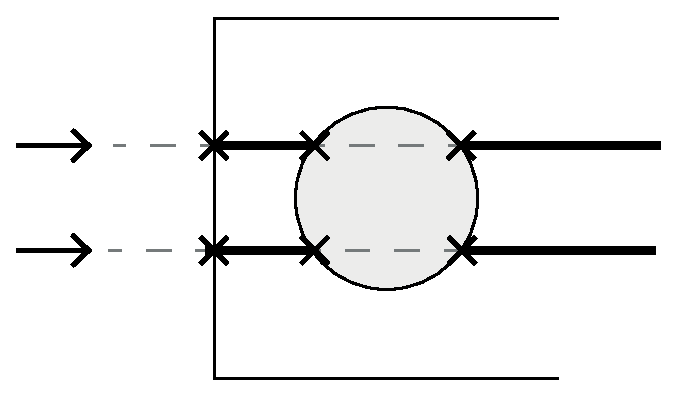
\includegraphics[width=\textwidth]{sections/methodology/figures/solid-non-watertight}
        \caption{Non-watertight 3D model cross section.}
        \label{fig:filling-non-watertight-model}
    \end{subfigure}
    \hfill
    \begin{subfigure}[b]{0.45\textwidth}
        \centering
        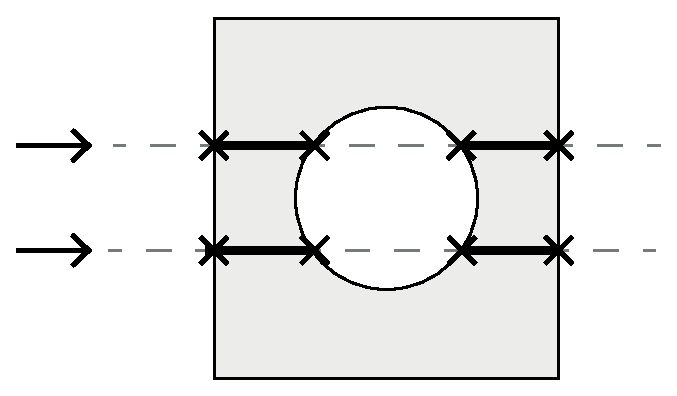
\includegraphics[width=\textwidth]{sections/methodology/figures/solid-watertight}
        \caption{Watertight 3D model cross section.}
        \label{fig:filling-watertight-model}
    \end{subfigure}
       \caption{Solid (voxelization) filling of 3D model cross section.}
       \label{fig:filling-3d-model}
\end{figure}

(\colorbox{RubineRed}{Remove watertight model?}) 

\subsection{three.js optimization}
The raycasting functionality, used by the raycasting algorithm described in Section \ref{sec:method-raycasting-algorithm}, is supplied by the three.js library. The library provides a throughly tested and accurate raycasting solution. However, it is CPU bound and  iterates every face of the mesh. This gives each raycasting operation a time complexity of O(n). If the 3D mesh is highly detailed, containing a large amount of polygons, the raycasting will take a long time to perform. After a careful assessment of potential solutions, the three.js plugin named three-bvh-mesh \cite{three-bvh-mesh} was used to improve this. This plugin provides a BVH implementation in order to speed up the raycasting against three.js meshes. By using this plugin, the time complexity for a single raycasting operation decreases from O(n) to O(log~n). Figure \ref{fig:bvh-monkey} shows an example visualization of a BVH tree applied to a 3D model, which is generated by the three-bvh-mesh plugin.

\begin{figure}[ht]
    \centering
    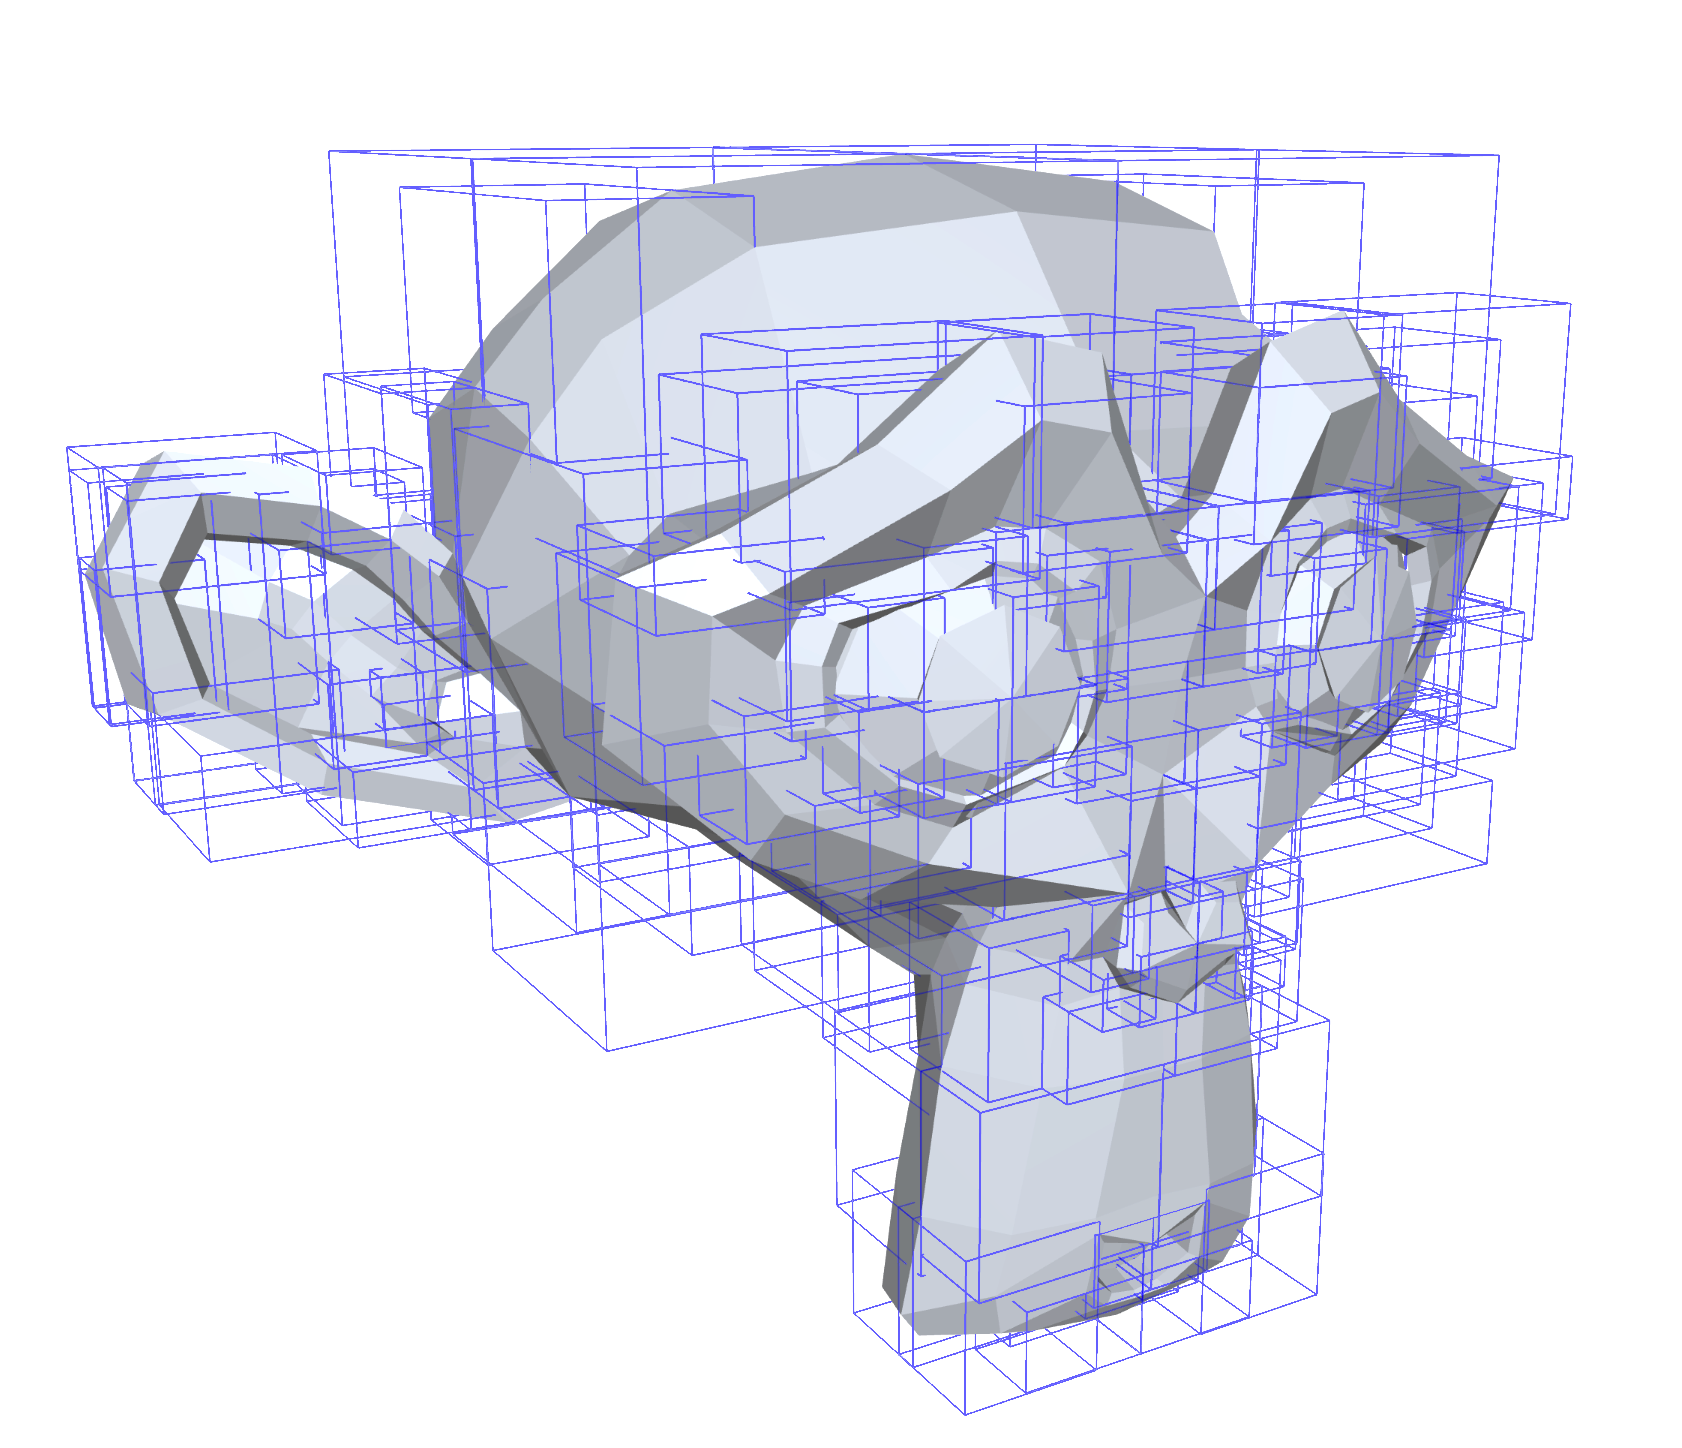
\includegraphics[width=0.5\textwidth]{sections/methodology/figures/bvh-monkey.png}
    \caption{Visualization of BVH applied to 3D model.}
    \label{fig:bvh-monkey}
\end{figure}

\subsection{Color system}
The color system of Voxelizer handles the storing and extraction of color from polygon meshes. This enables the engine to extract color information from the 3D mesh, and apply it to the voxels. The system mainly comprises of a ColorExtractor class and a TextureHandler class. The TextureHandler class stores a copy of all the texture maps associated with a 3D object. These are stored in a hashmap, using the texture maps UUID as key. Further, it is able to look up a UV coordinate of a texture map in its store, retrieving the corresponding color. See Section~\ref{sec:info-texture-maps} for more details on texture maps and UV coordinates. The ColorExtractor class provides various methods for extracting colors from from an raycast intersect. It uses the TextureHandler as internally texture storage, for fast lookup of texture colors. 

During raycasting with the raycasting algorithm described in Section~\ref{sec:method-raycasting-algorithm}, each intersect produces an UV coordinate of the associated texture map, along with its UUID. This info is then fed to a ColorExtractor class, returning the appropriate RGB color of the intersect. This color data is then stored in a four-dimensional view of a large ndarray. For maximum efficiency and safety, actual datatype supplied to ndarray is an Uint8ClampedArray~\cite{uint8clampedarray} (typed array).

\subsection{Loading}
The Voxelizer library/engine previously made use of a wrapper OBJ loader. This resulted in very limiting compatibility with other file formats. This support has been dropped in favor of the new ES6 JS loader modules introduced by three.js. three.js supports around 40 different file formats for loading 3D models. All three.js objects inherits from a base class named Object3D. This includes meshes. By ensuring compatibility with three.js meshes, any loader compatible with three.js can be used.

\subsection{Exporting}
As described in Section~\ref{sec:method-implementation}, the engine normally outputs ndarrays with color and voxel information, wrapped in a Volume class. However, the engine also comes with several exporter classes. This includes:
\begin{itemize}
    \item \textbf{XML} - XML provides a versatile and flexible file format. The native JavaScript DOM parser is used for the actual parsing of the XML data. The outputted format of the XML document structure is described on the GitHub wiki page for the engine.
    \colorbox{red}{PROVIDE LINK HERE !!!}
    \item \textbf{BINVOX} - BINVOX~\cite{binvox-file-format} is one of the more popular voxel data file formats. BINVOX is the file format used by the binvox~\cite{binvox} voxelization software. A separate repository named binvox~\cite{andstor-binvox} has been created for handling BINVOX files. See Section~\ref{sec:method-binvox}.
    \item \textbf{3D array} - An array exporter is implemented for exporting the voxel data as a normal nested JavaScript array. If the export includes color data, this is exported as a 4D JavaScript array.
\end{itemize}

\subsection{Testing}
Several unit tests are created for testing the different parts of the voxelization system. This ensures correct operation of the voxelization process, and protect against introducing new bugs. Jest~\cite{jest} has been chosen as the testing framework provider. Jest also provides coverage reports. These are very valuable in terms of analyzing what parts of the system is and is not tested.

\subsection{Migration}
The previous version of Voxelizer was version v0.1.3. Following Semantic Versioning~\cite{semantic-versioning}, or SemVer, the old version of Voxelizer is defined as still in Beta. Introducing a new Major version of the library with breaking functionality is therefore no problem. Still, a very simple migration guide is provided on the Wiki of the Voxelizer engine repository on GitHub \colorbox{red}{LINK HERE!!!!}.

\subsection{Debugging and Profiling}
During development, the three-voxel-loader plugin was used to visualize the actual voxel outputs. This made it easy to visually inspect the results of the voxelization algorithm. A similar solution to the debugging setup used for the three-voxel-loader plugin was used. Likewise, this also resulted in an example usage of the engine, and is deployed to GitHub Pages. \colorbox{red}{LINK TO VOXELIZER EXAMPLE PAGE}.

For assessing the memory consumption and speed of the engine, the performance tool~\cite{chrome-dev-tools-profiler} in the Google Chrome Developer Tools is used. This helped removing some CPU-heavy bugs, memory issues and other performance bottlenecks. Figure~\ref{fig:chrome-devtools-performance} shows an image of the performance tool.

\begin{figure}[ht]
    \centering
    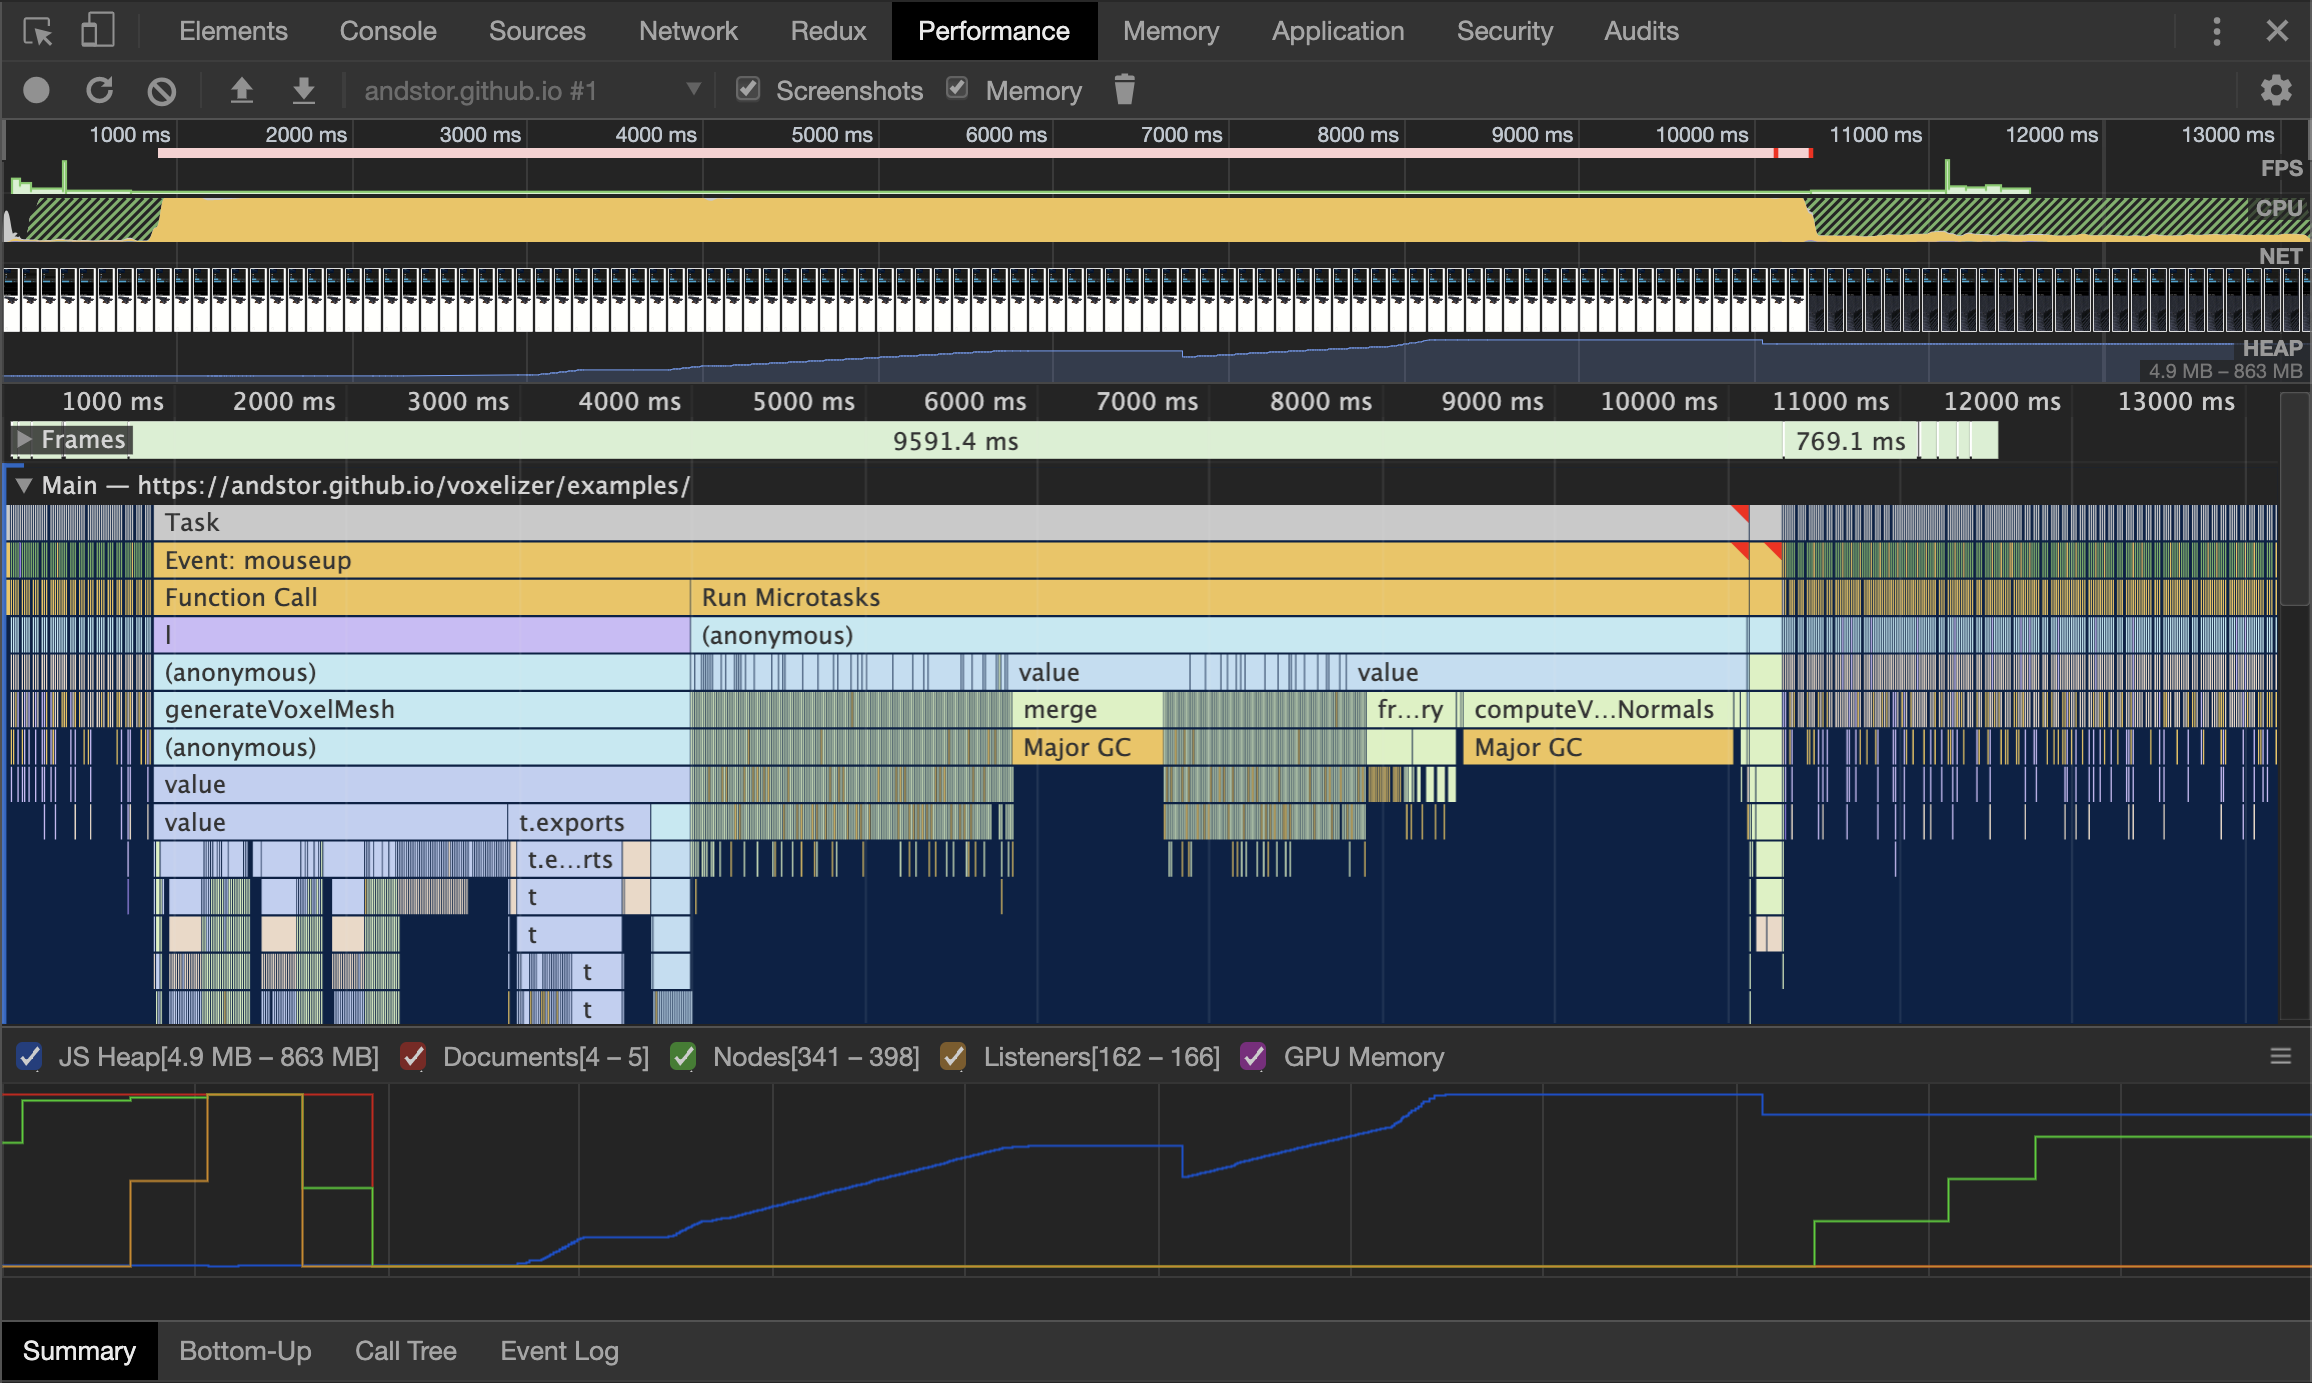
\includegraphics[width=\textwidth]{sections/methodology/figures/chrome-dev-tools-performance.png}
    \caption{Screenshot of performance profiling with Google Chrome Developer Tools.}
    \label{fig:chrome-devtools-performance}
\end{figure}

\subsection{Building}
The engine is bundled with Webpack. This gives great control over the building process. See Section~\ref{sec:theory-bundling} for more details on Webpack. Voxelizer also makes use of ES6 features, so all source files are also transpiled to ES5 with babel. The main output of the library is UMD, as described in Section~\ref{sec:theory-module-system}. This makes the engine compatible with a range of other module systems. However, since Webpack does not support ES Modules right out of the box, a better alternative would be to use Rollup \ref{sec:theory-bundling}. Unfortunately, this was not possible due to a circular dependency in one of the dependencies of Voxelizer. Therefore, in order to use Voxelizer as a native ES Module, a project also needs to use a module loader like Webpack.

\section{BINVOX}
\label{sec:method-binvox}
A separate open-source repo for building and parsing BINVOX file formats were created during refactoring of the Voxelizer engine and the three-voxel-loader plugin. It is named binvox and licensed under the MIT license. The BINVOX file format consists of a header in plain ASCII, followed by binary data. The binary data is compressed using run-length encoding. From the BINVOX specification: \textquote[\citet{binvox-file-format}]{The binary data consists of pairs of bytes. The first byte of each pair is the value byte and is either 0 or 1 (1 signifies the presence of a voxel). The second byte is the count byte and specifies how many times the preceding voxel value should be repeated (so obviously the minimum count is 1, and the maximum is 255).}.

The new binvox package provides tools to both parse and construct files according to the BINVOX file specification~\cite{binvox-file-format}. Parsing is done on the individual set of two bits, uncompressing the data and storing it in a JSON format. An example of the parsed JSON result can be seen in Program~Code~\ref{lst:binvox-example}. Similarly, a user can supply the same JSON data structure for constructing a BINVOX file resource. Hence, parsing and building commute.
\lstinputlisting[language=JSON,style=numbers,label={lst:binvox-example},caption={Example BINVOX data in JSON format}]{sections/methodology/code/binvox-json.json}

\section{Voxelizer-Desktop}
\colorbox{red}{WRITE THIS SECTION!!!!}
\subsection{Electron}
\subsubsection{Auto updating}

\subsection{GUI}
... Sketches?? Wireframe diagrams of GUI etc...


\section{JSDoc Action}
In the next couple of subsections, the implementation and design decisions of the JSDoc Action will be presented.
\subsection{Implementation}
For creating a GitHub Action, several mandatory files and configurations has to be created. This documentation is available at GitHub. GitHub Actions provides two main types of action. One is JavaScript based. The other is based on Docker. They both have their advantages and disadvantages. A Docker container action provides an isolated environment, providing extremely flexible and stabile solutions. However, it is only possible to run on Linux. On the other hand, a JavaScript GitHub Action can be run directly on a runner machine. This makes it a lot faster than a Docker based Action. This is because of latency due to retrieve and build the container. A JavaScript action is also cross platform compatible, meaning it can run on both a Linux, Windows or MacOS operating system. In order to provide a fast and cross compatible solution, the JavaScript action type is chosen for the JSDoc Action.

The JSDoc Action is made up of mainly two parts. One is the template installation system, and the other is the actual execution of the JSDoc tool. For providing maximum flexibility, all functions of the JSDoc tool is made available as input configurations through the GitHub Actions Workflow API. The action is also able to use a JSDoc configuration file \cite{jsdoc-config-file}. If a user provides a template to be installed, the action will first install this. This is done with the help of the node package manager (npm). The supplied template can be everything from a GitHub repository, to an npm package. The installed template files are then processed. The action does all of its IO operations asynchronously, ensuring fast execution speed of the action. When finished, a JSDoc CLI command is then formed based on the various user inputs and (if provided) config file. This command is then executed, effectively telling JSDoc to generate the documentation. The result is a user defined output folder with the generated API documentation.

\subsection{Usage}
For actually using the action in a Workflow, the action makes a couple of assumptions. Firstly, the actual source files to generated documentation from needs to be supplied. This is normally solved by using the Checkout~Action~\cite{checkout-action} made by GitHub. Secondly, the JSDoc Action only generates an output directory with files. This means that nearly any deployment action can be used for upload the files the desired service, for example GitHub pages. The deployment action supplied as example in the README.md file of the repository is named GitHub~Pages~Action~\cite{github-pages-action}.

\subsection{Feedback}
The JSDoc Action generated quite a lot of feedback from eager users of the action. Several wanted to test the action, and multiple issues were filed in the issue tracker on GitHub~\cite{jsdoc-action-issue-tracker}. See for example issue~\#20~\cite{jsdoc-issue-20}. Since maintenance is essential to the success of an open-source project, all feedback were responded to and handled accordingly. Alongside the development of the other main projects, many bug-fixes were made to the JSDoc Action. Eventually, all issues were resolved, resulting in several happy users.


\section{Automation}
Automation is an important part for ensuring both efficiency and security. The next subsections will contain a description of how the various open-source systems developed in connection with this thesis have been automated.

\subsection{JavaScript package workflows}
\label{sec:method-javascript-package-workflows}
GitHub provides CI and CD as a part of its GitHub Actions system. This system has been put to use, creating several workflows in order to automate various tasks like testing, building, documentation generation and publishing. The workflows have been made so that they should work out of the box for similar projects. See Section~\ref{sec:theory-github-actions} for a description of GitHub Actions. Do note that the default behavior of Workflows is to terminate if any errors are encountered.

Figure~\ref{fig:cicd-pipelines} shows a simplified diagram of the CI/CD automation pipelines created for the JavaScript packages which are to run on new contributions to the codebase. This system mainly consists of two workflows. One for building the package, and one for generating and publishing API documentation. A simple step by step walkthrough of the system is now presented.

\begin{enumerate}
    \item \textbf{Pull request} - The pipelines are mainly triggered by a pull request. This starts up both a security analysis by LGTM and a build workflow.
    \item \textbf{Security analysis} - As described in Section~\ref{sec:theory-semmle-lgtm}, LGTM provides a security analysis. If any vulnerabilities are found, the pull request fails.
    \item \textbf{Build workflow} - The build workflow has four steps.
    \begin{enumerate}
        \item \textbf{Checkout} - First, the repository in which the automation is done on is cloned.
        \item \textbf{Build} - Then, the JavaScript project is built.
        \item \textbf{Test} - If the project provides tests, these are also run.
        \item \textbf{Coverage} - Coverage reports are created with Jest.
    \end{enumerate}
    \item \textbf{Coveralls} - The coverage report is then published to Coveralls.io. See Section~\ref{sec:theory-coveralls} for details on Coveralls.
\end{enumerate}

If the workflow finishes, the security analysis comes out clear, and the coverage percentage is not decreased, the pull request is approved for merging. When a user with the appropriate privileges approves the pull request, the code is merged into the base branch. If the base branch is the master branch, a second workflow is started. This is a workflow for generating/updating the API documentation.

\begin{enumerate}
    \item \textbf{Checkout} - The source repo is cloned once again.
    \item \textbf{JSDoc Action} - The JSDoc Action is then used for generating JSDoc API documentation.
    \item \textbf{GitHub Pages} - The outputted documentation is then finally deployed to GitHub Pages with an action called \cite{github-pages-action}.
\end{enumerate}

\begin{figure}[hp!]
    \setlength{\abovecaptionskip}{25pt}
    \centering
    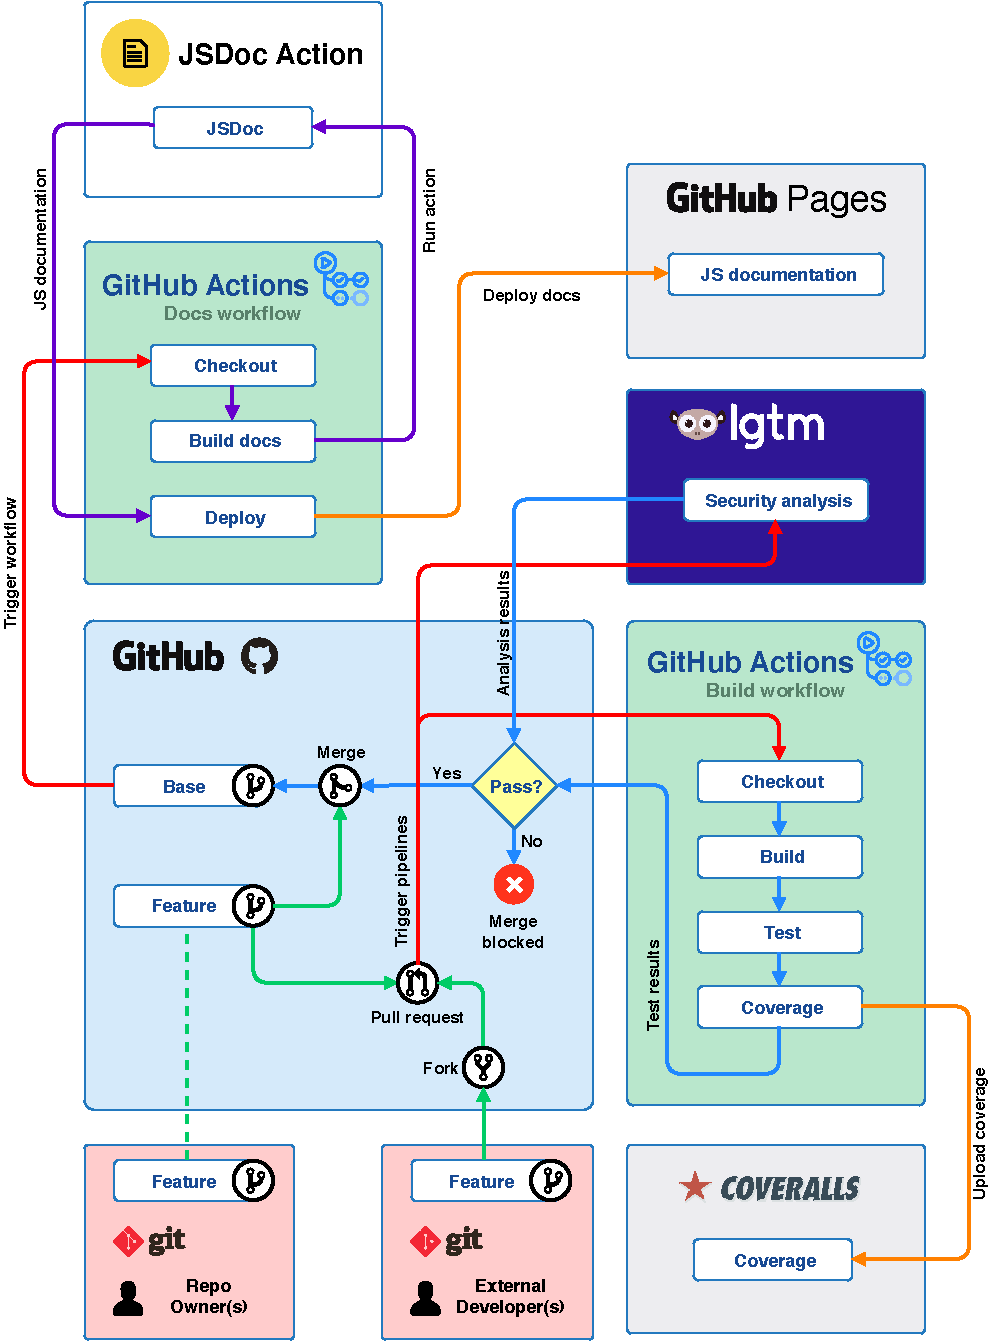
\includegraphics[page=1,scale=1]{sections/methodology/figures/pipelines.pdf}
    \caption{CI/CD pipelines}
    \label{fig:cicd-pipelines}
\end{figure}
%\clearpage

In order to automate the release process of a JavaScript package, a third workflow is used. This is shown in Figure~\ref{fig:release-automation}. It mainly involves packaging and publication of the software to the npm~registry~\cite{npm-registry}. The workflow functions like this:
\begin{enumerate}
    \item \textbf{Trigger release} - First, a user with the appropriate privileges needs to create a release manually on GitHub. This generates a git tag. Further, the release starts up the package workflow.
    \item \textbf{Package workflow}
    \item \begin{enumerate}
        \item \textbf{Checkout} - The source repo is cloned once again.
        \item \textbf{Build} - The JavaScript project is then built.
        \item \textbf{Test} - If the project provides tests, these are also run.
        \item \textbf{Package} - If all the above tests are completed without errors, the project is then packaged.
    \end{enumerate}
    \item \textbf{Publish package} - If the package workflow completes, the new package is then published to the npm registry.
\end{enumerate}

\begin{figure}[hp]
    \setlength{\abovecaptionskip}{25pt}
    \centering
    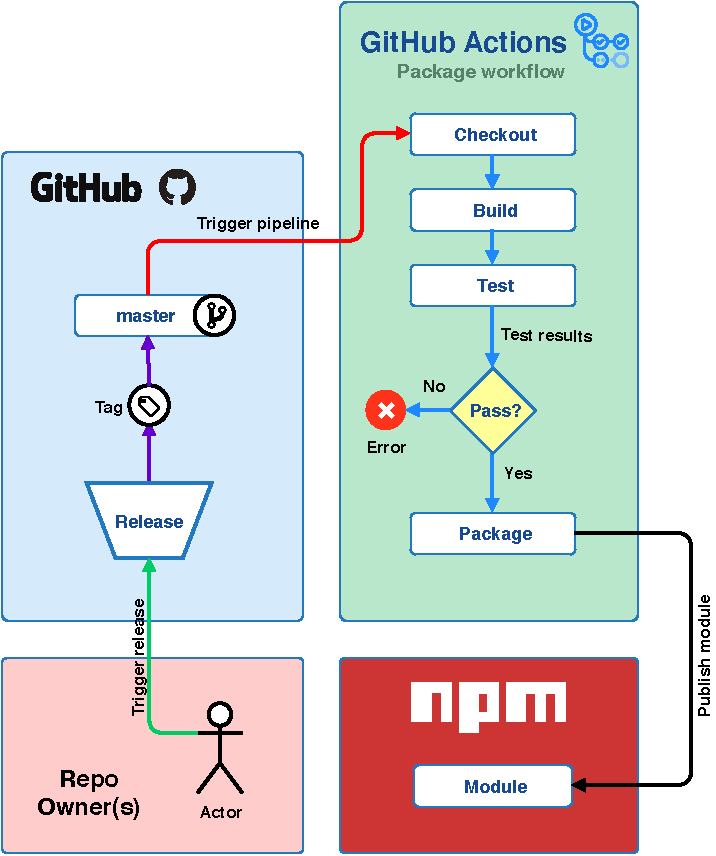
\includegraphics[page=1,scale=1]{sections/methodology/figures/package-release-automation.pdf}
    \caption{Automation of release publishing process.}
    \label{fig:release-automation}
\end{figure}

\subsection{GitHub Action version tagging}
GitHub provides guidelines in terms of versioning and tagging of a GitHub Actions \cite{github-actions-versioning}. According to Github, releases should be following Semantic Versioning. When a new release is made, the major tag (v1, v2, etc.) should be moved to point on the Git ref of the current release. This process is tedious. A workflow has therefore been created for automating this release process. Figure~\ref{fig:update-major-tag} provides an illustration of the moving of Git tags. An action named actions-tagger~\cite{actions-tagger} already provides support for this tagging scheme.

Following
Auto major version tagging update

\begin{figure}[hp]
    \setlength{\abovecaptionskip}{25pt}
    \centering
    \hspace*{-2cm}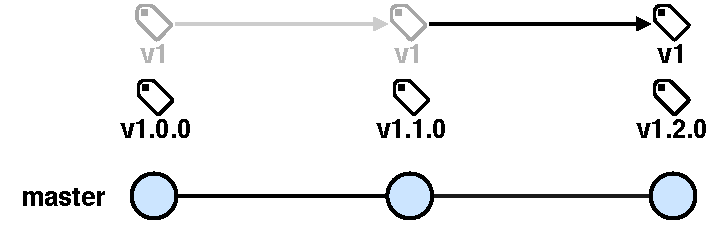
\includegraphics[page=1,scale=1]{sections/methodology/figures/update-major-tag.pdf}
    \caption{Automatic updating of major version tag.}
    \label{fig:update-major-tag}
\end{figure}

\section{file-existence-action}
\label{sec:method-file-existence-action}
In order to be able to produce the general purpose workflows described in Section~\ref{sec:method-javascript-package-workflows}, it became apparent that i needed to be able to check if a file existed. Normally, a coverage script is defined in the projects package.json file. This runs all the tests and produces a coverage report file. However, if no such script is provided, the workflow will run the tests manually instead, and no file will be generated. If no such file is generated, this needs to be detected by the workflow, in order to avoid running the upload to Coveralls.io step. This resulted in a relatively small GitHub Action, named File Existence. The action is written in TypeScript, and based on a template provided by GitHub. The action is able to check one or more paths for the existence of a file. The boolean result is then available to the following steps in the workflow.

\section{file-reader-action}
Following the problems described in Section~\ref{sec:method-file-existence-action} above, another problem arises if the coverage script is defined, but no tests are created. If this is the case, an empty coverage file is created. Trying to upload this to Coveralls.io results in an error. The need for reading the contents of a file was therefore necessary, in order to check if the coverage file is empty. If it is empty, the Coveralls step should not be executed. The solution was to create a small GitHub Action, named File Reader. The action is written in TypeScript, and based on a template provided by GitHub. The action is able to read the contents of a file path supplied by the user. THe output is then available to the consequently workflow steps.
%This is chapter 4
%%=========================================
\chapter{Result}
This chapter presents the results of this project. \colorbox{red}{SOME MORE HERE?}

Due to various extra work like the binvox package, the file-existence-action and the file-reader-action, some functionality had to give way to others. It was simply not enough time to make the CLI tool for the Voxelizer engine.

The chapter starts with presenting the various results from the different projects developed and connection with this thesis. First, the new three-voxel-loader three.js plugin and the improvements of the Voxelizer engine are presented. This is followed by the new BINVOX package, and the desktop application for the Voxelizer engine. Then, the results of the JSDoc GitHub Action is presented

\section{three-voxel-loader}
The three-voxel-loader is a plugin for three.js. It is published to the npm registry under the name "three-voxel-loader", and the source code is available at GitHub under "andstor/three-voxel-loader".

The plugin is able to generate a three.js mesh based on voxel data in a variety of data formats. Figure~\ref{fig:three-voxel-loader} shows a screenshot of a VOX model loaded with the three-voxel-loader plugin.
\begin{figure}[htp]
    \centering
    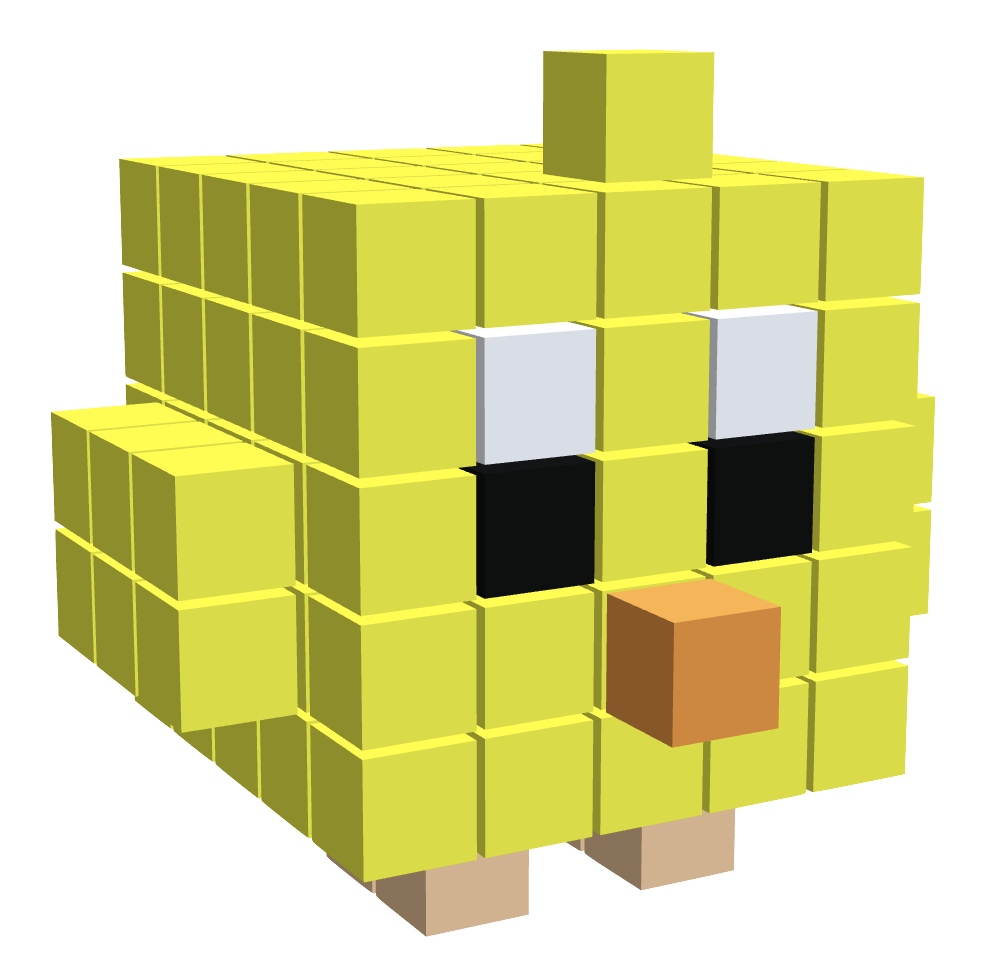
\includegraphics[width=0.45\textwidth]{sections/result/figures/chicken-voxels.png}
    \caption{Screenshot of Chicken stored in VOX file format loaded with the three-voxel-loader plugin.}
    \label{fig:three-voxel-loader}
\end{figure}
It is also possible to control the size of the individual voxels. This is shown in Figure~\ref{fig:chicken-voxels-sizes}. The size can be any number between $\left<0, 1\right]$.
\begin{figure}[htp]
    \centering
    \begin{subfigure}[t]{0.45\textwidth}
        \centering
        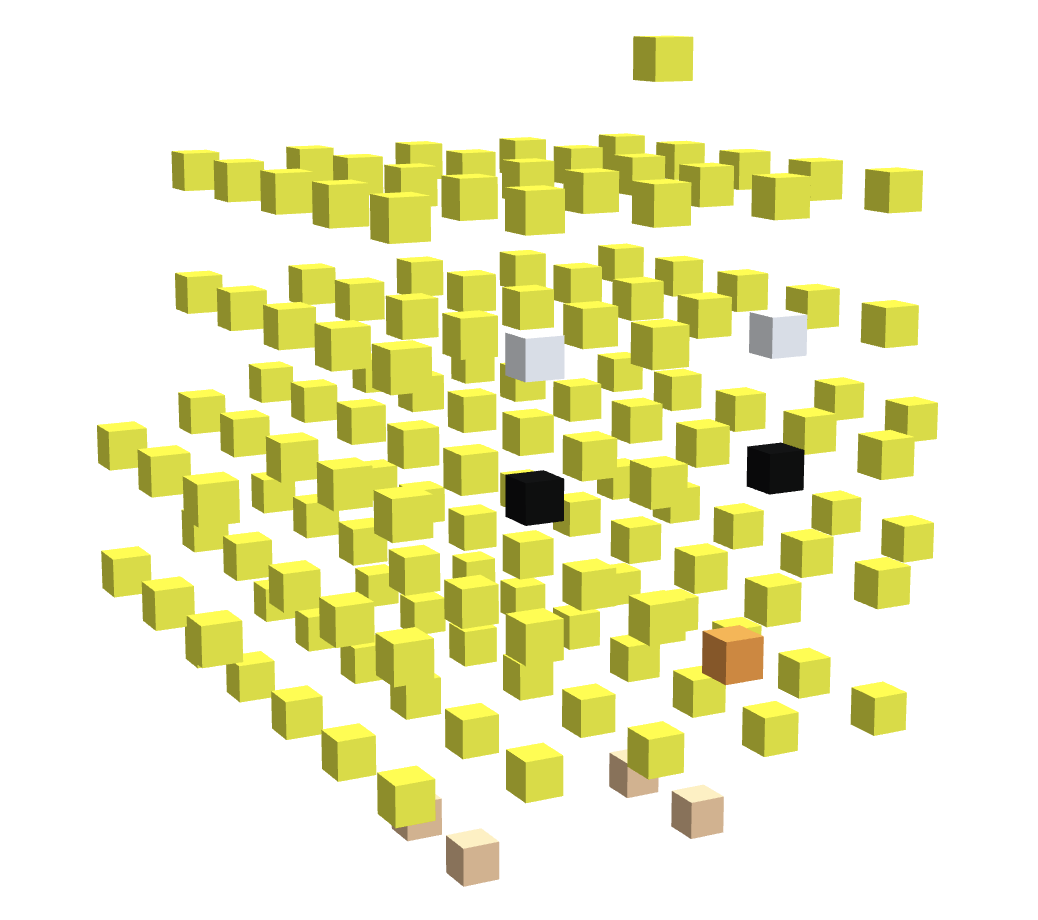
\includegraphics[width=\textwidth]{sections/result/figures/chicken-voxels-size-0.3.png}
        \caption{Voxel size set to 0.3.}
        \label{fig:chicken-voxels-size-0.3}
    \end{subfigure}
    \hfill
    \begin{subfigure}[t]{0.45\textwidth}
        \centering
        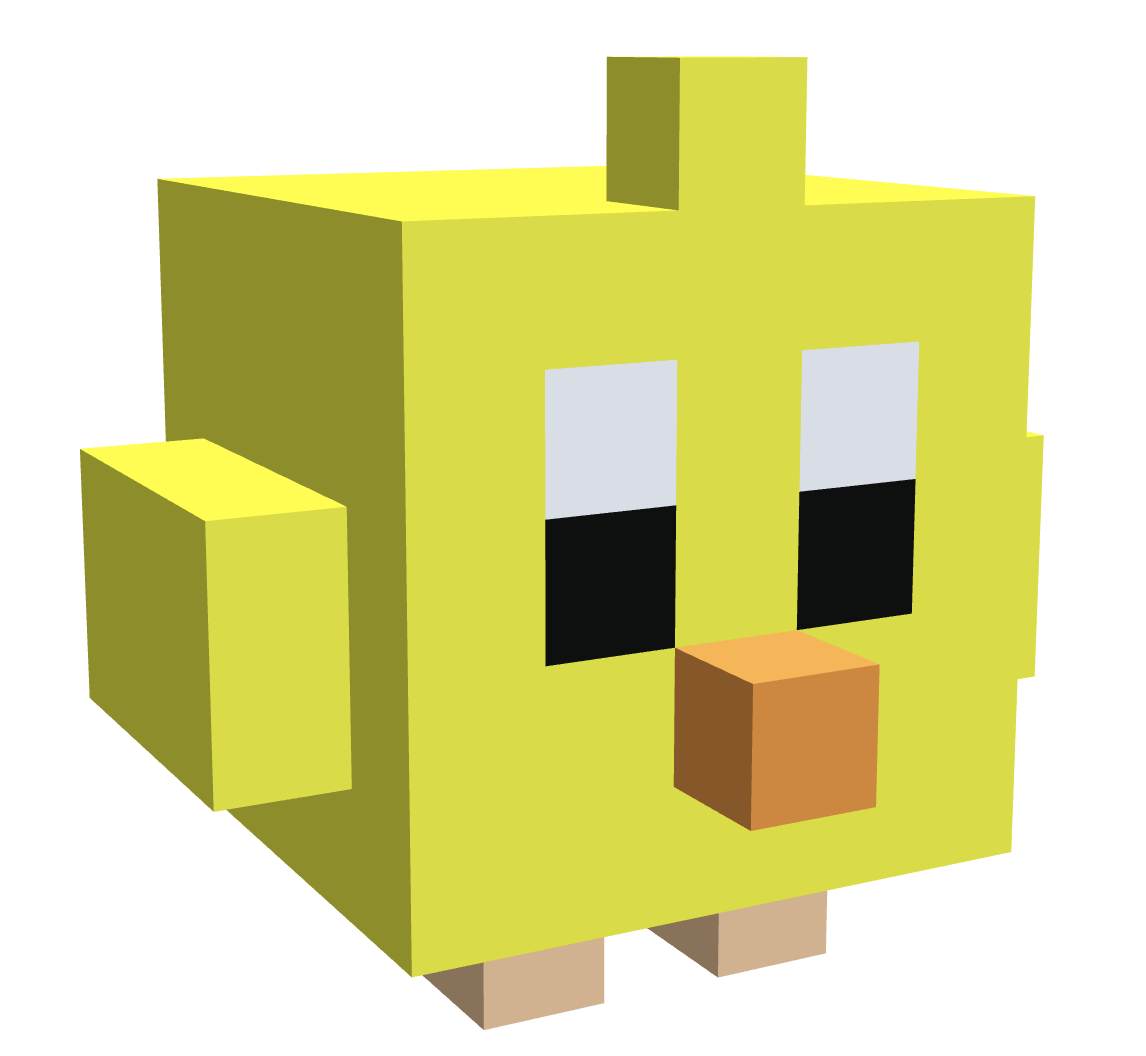
\includegraphics[width=\textwidth]{sections/result/figures/chicken-voxels-size-1.png}
        \caption{Voxel size set to 1.}
        \label{fig:chicken-voxels-size-1}
    \end{subfigure}
       \caption{Generated meshes with different voxel sizes.}
       \label{fig:chicken-voxels-sizes}
\end{figure}


\subsection{Level Of Detail}
The plugin implements a Level Of Detailing (LOD) system. Figure~\ref{fig:torus-lod} shows four images of a torus loaded with different LODs. Depending of the resolution of the model, a very high number of triangles may be generated. By using the LOD system, this number can be drastically reduced. For example, the mesh in Figure~\ref{fig:torus-lod-10} consists of 406,068 triangles. By setting the LOD (maxDepth) to 2, the number is reduced to only 768 triangles, still preserving the shape. This can be seen in Figure~\ref{fig:torus-lod-2}.
\begin{figure}[htp]
    \centering
    \begin{subfigure}[t]{0.45\textwidth}
        \centering
        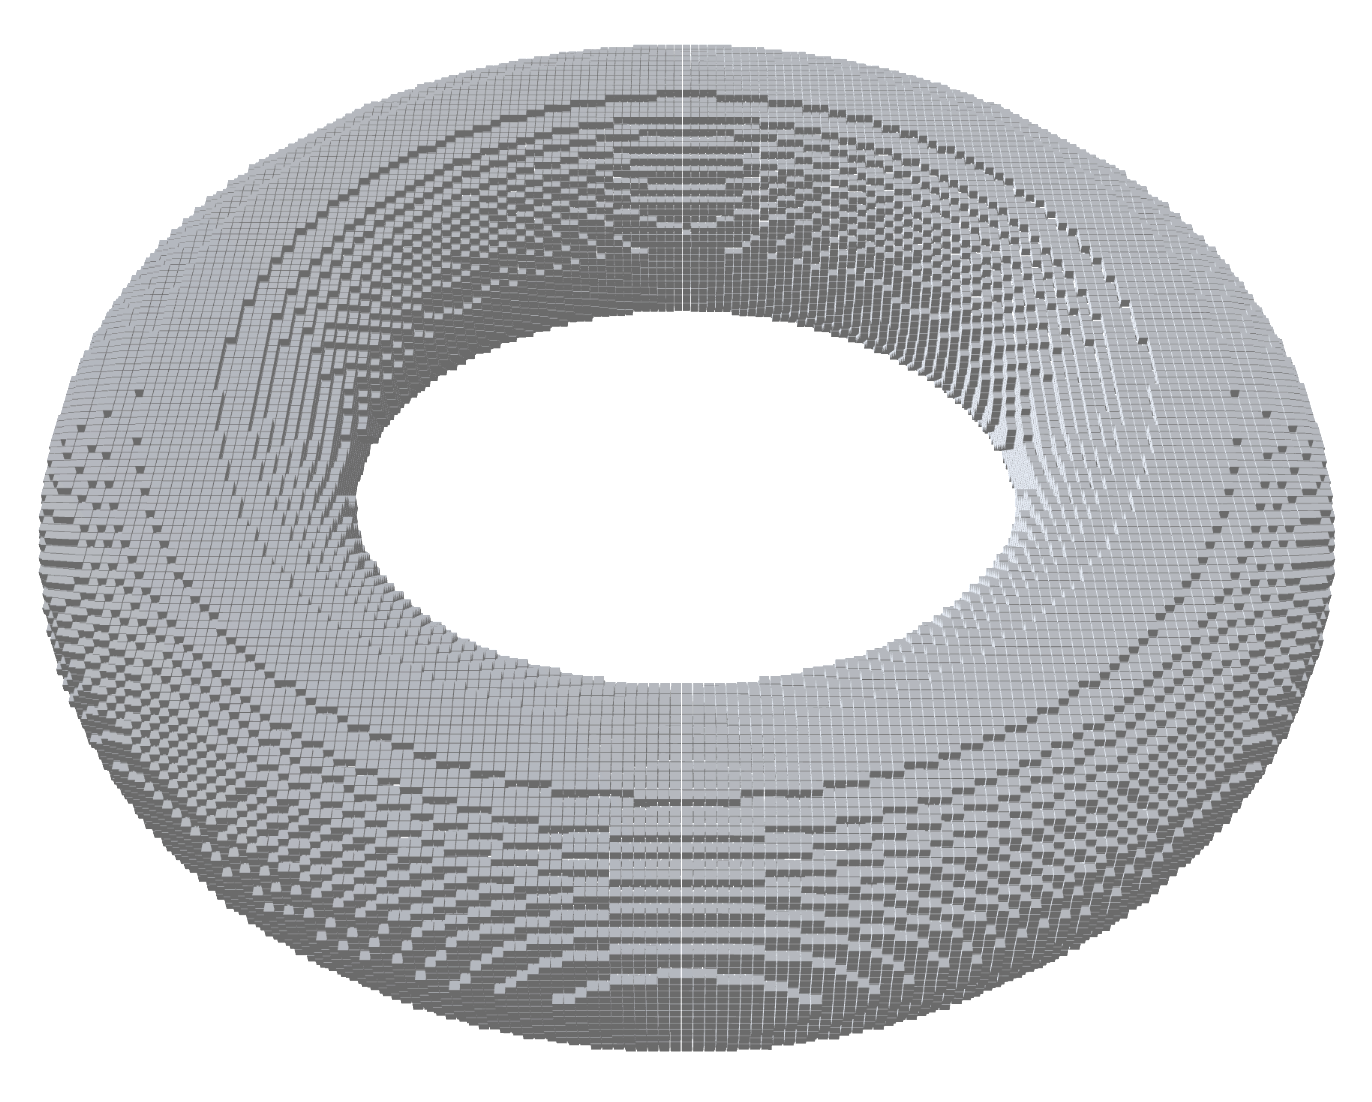
\includegraphics[width=\textwidth]{sections/result/figures/torus-lod-10.png}
        \caption{Full resolution torus mesh (406068~triangles).}
        \label{fig:torus-lod-10}
    \end{subfigure}
    \hfill
    \begin{subfigure}[t]{0.45\textwidth}
        \centering
        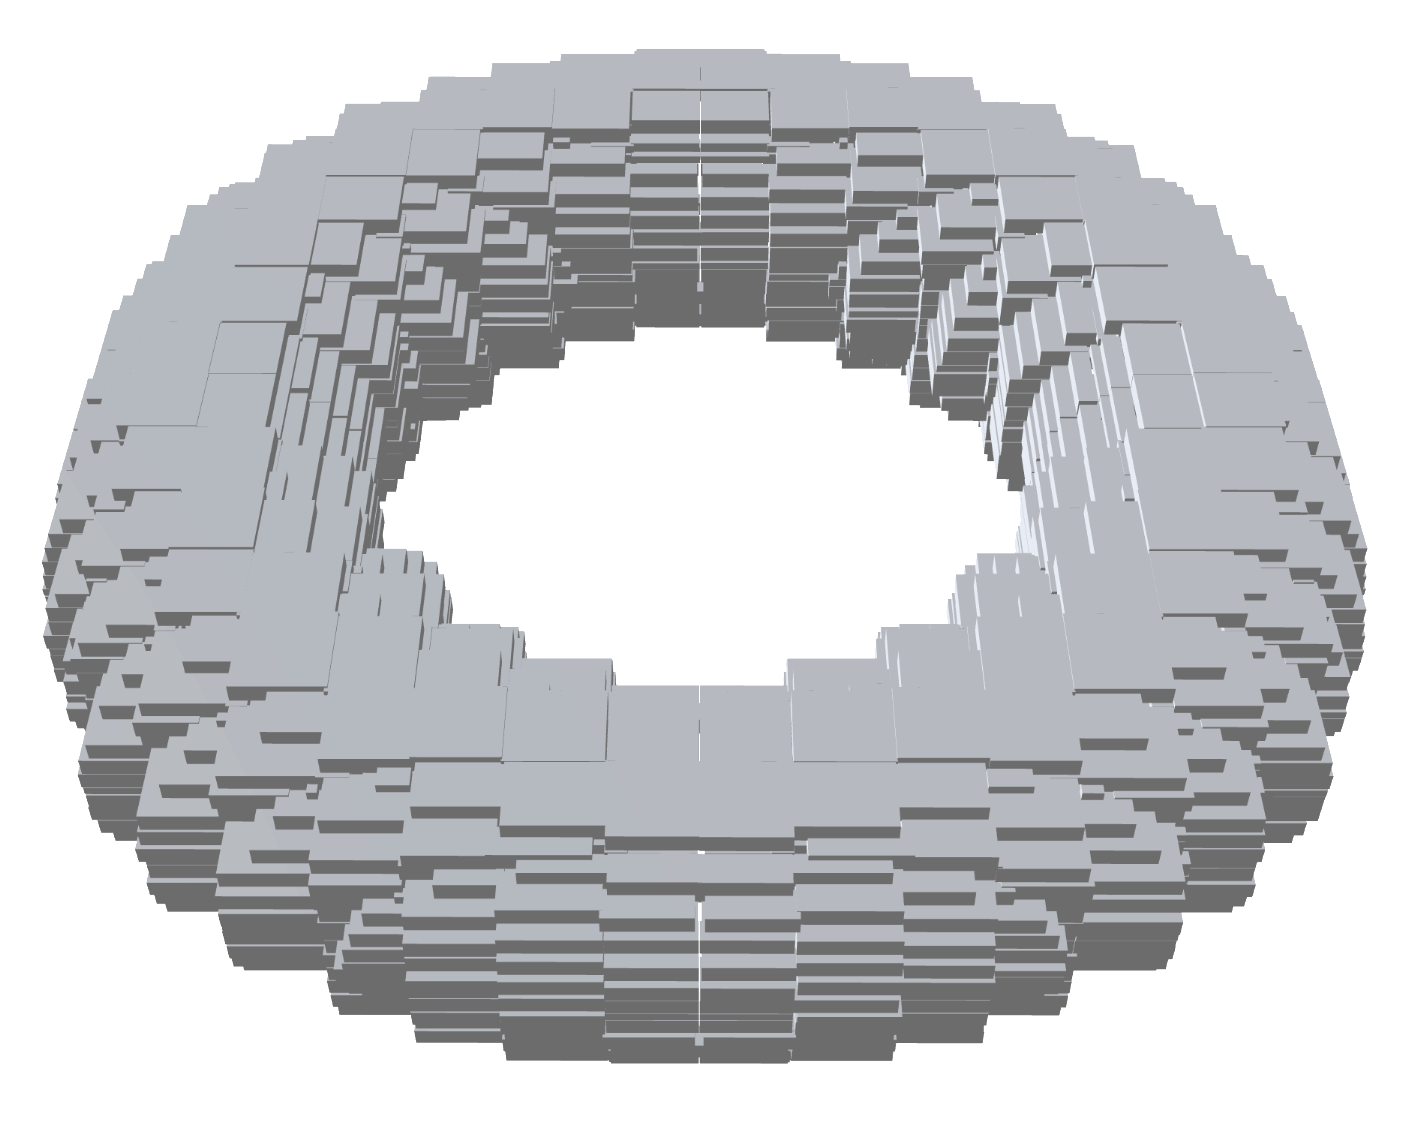
\includegraphics[width=\textwidth]{sections/result/figures/torus-lod-4.png}
        \caption{Simplified torus mesh (19740~triangles) with a LOD (maxDepth) of 4.}
        \label{fig:torus-lod-4}
    \end{subfigure}
    \hfill
    \begin{subfigure}[t]{0.45\textwidth}
        \centering
        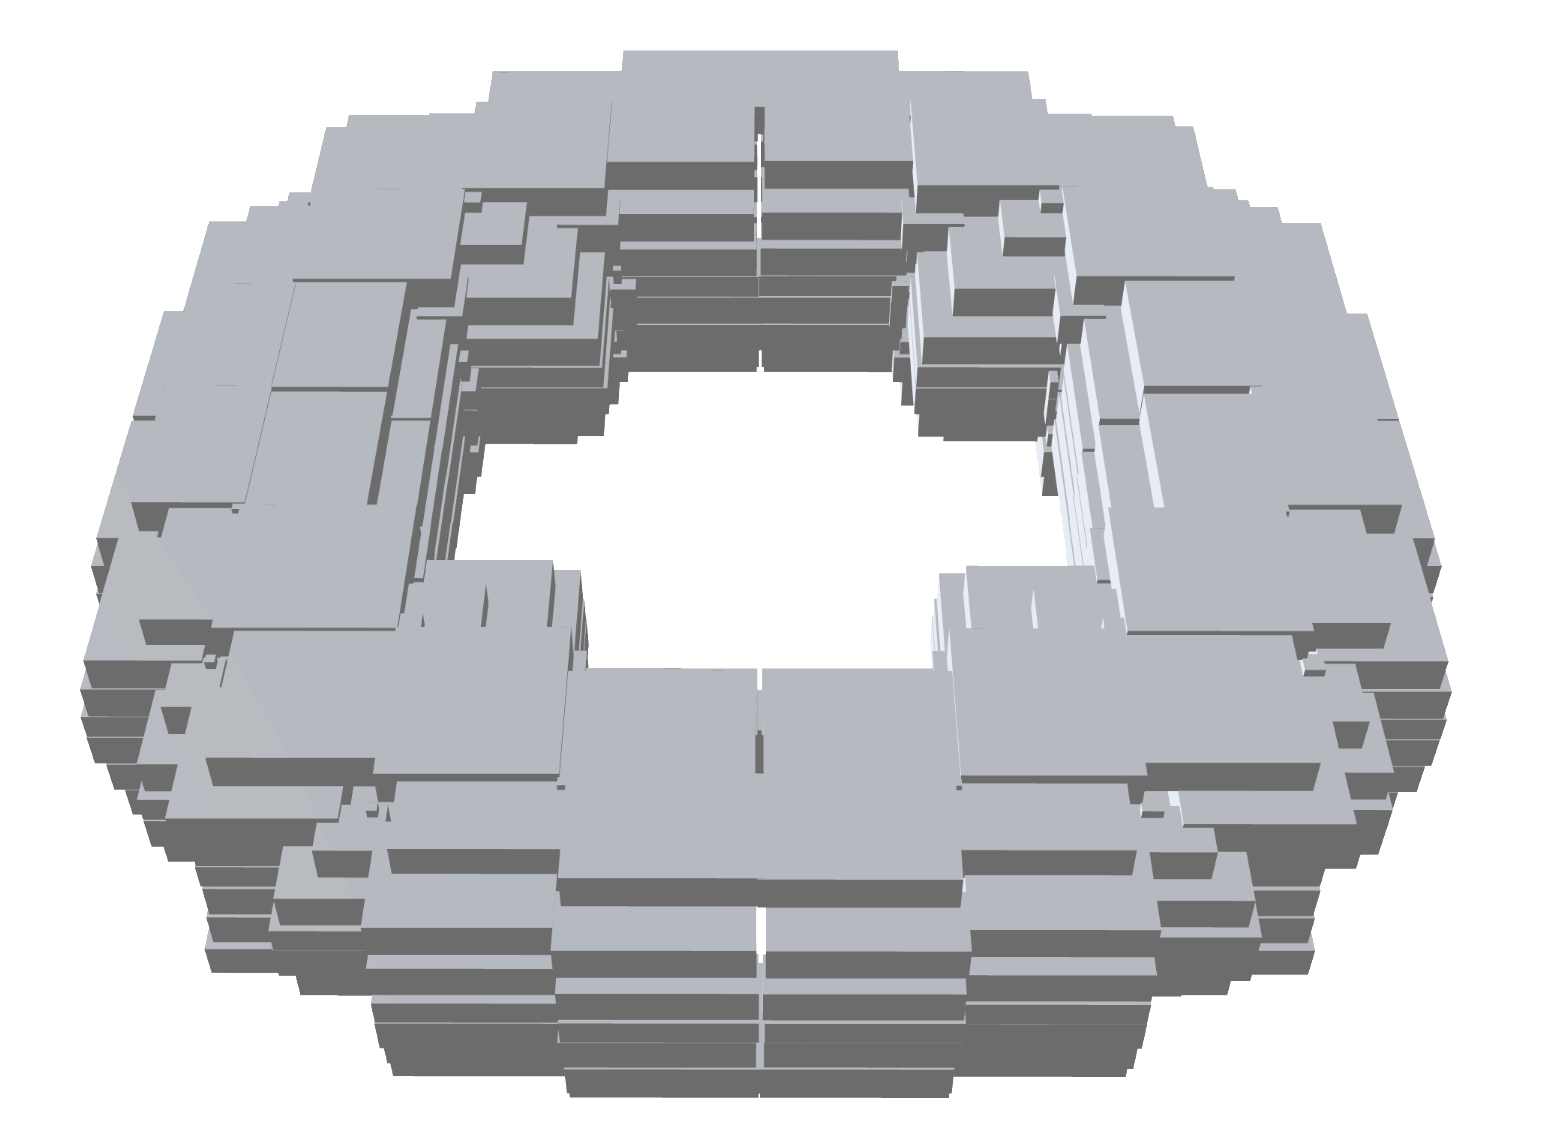
\includegraphics[width=\textwidth]{sections/result/figures/torus-lod-3.png}
        \caption{Quite simplified torus mesh (4752~triangles) with a LOD (maxDepth) of 3.}
        \label{fig:torus-lod-3}
    \end{subfigure}
    \hfill
    \begin{subfigure}[t]{0.45\textwidth}
        \centering
        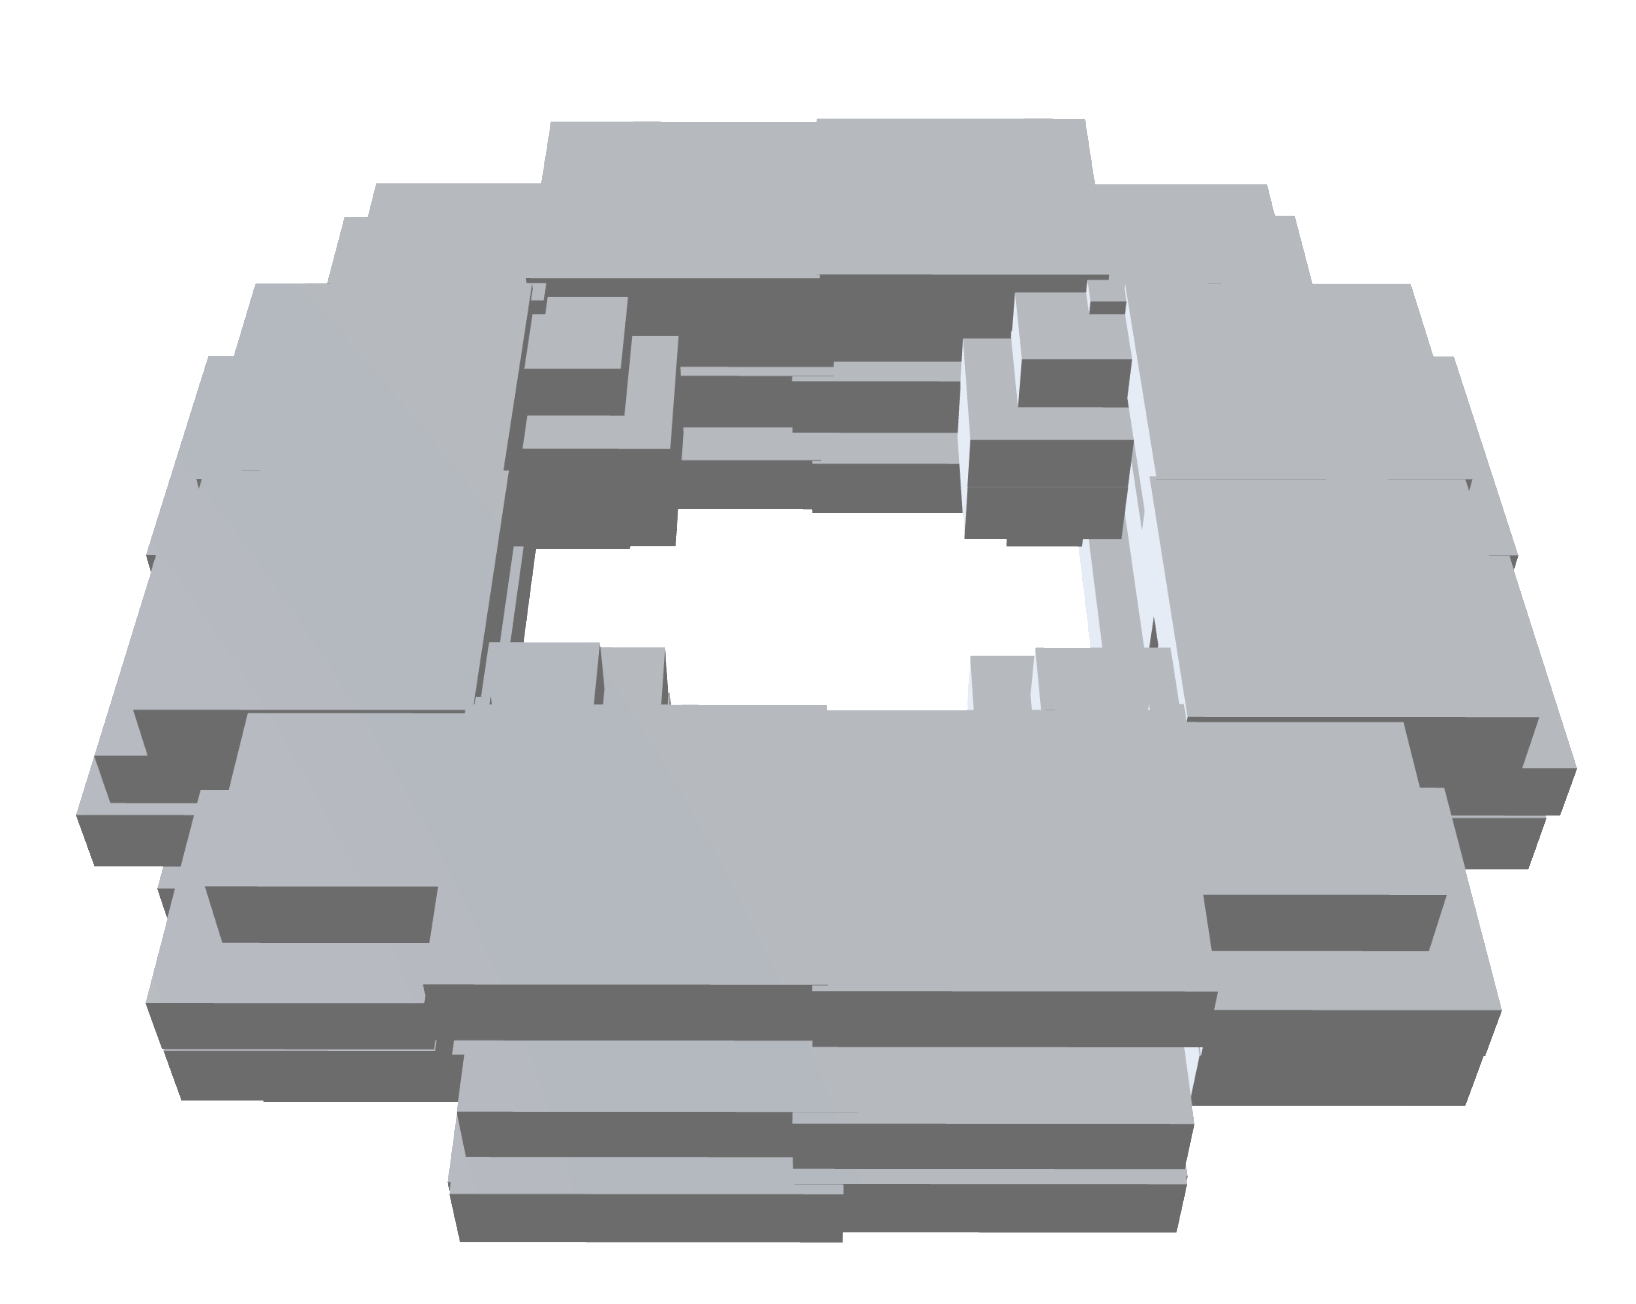
\includegraphics[width=\textwidth]{sections/result/figures/torus-lod-2.png}
        \caption{Very low detail torus mesh (768~triangles) with a LOD (maxDepth) of 2.}
        \label{fig:torus-lod-2}
    \end{subfigure}
       \caption{Torus meshes with diffrent LOD levels.}
       \label{fig:torus-lod}
\end{figure}

\subsection{Loading support}
The plugin is able to load a variety of different voxel data formats. This includes XML, VOX, BINVOX and JavaScript arrays (3D array). In addition to the raw voxel data, the three-voxel-loader plugin also supports color. The data formats that support this is XML, VOX and JavaScript arrays (4D array for color data).

\subsection{Example}
An example of the plugin is deployed to GitHub Pages. Visit \url{https://andstor.github.io/three-voxel-loader/examples/} to see the example. Figure~\ref{fig:three-voxel-loader-example} shows a screenshot of the site. The example includes a GUI with controls for changing, among other things, the voxel size and the LOD.
\begin{figure}[ht]
    \centering
    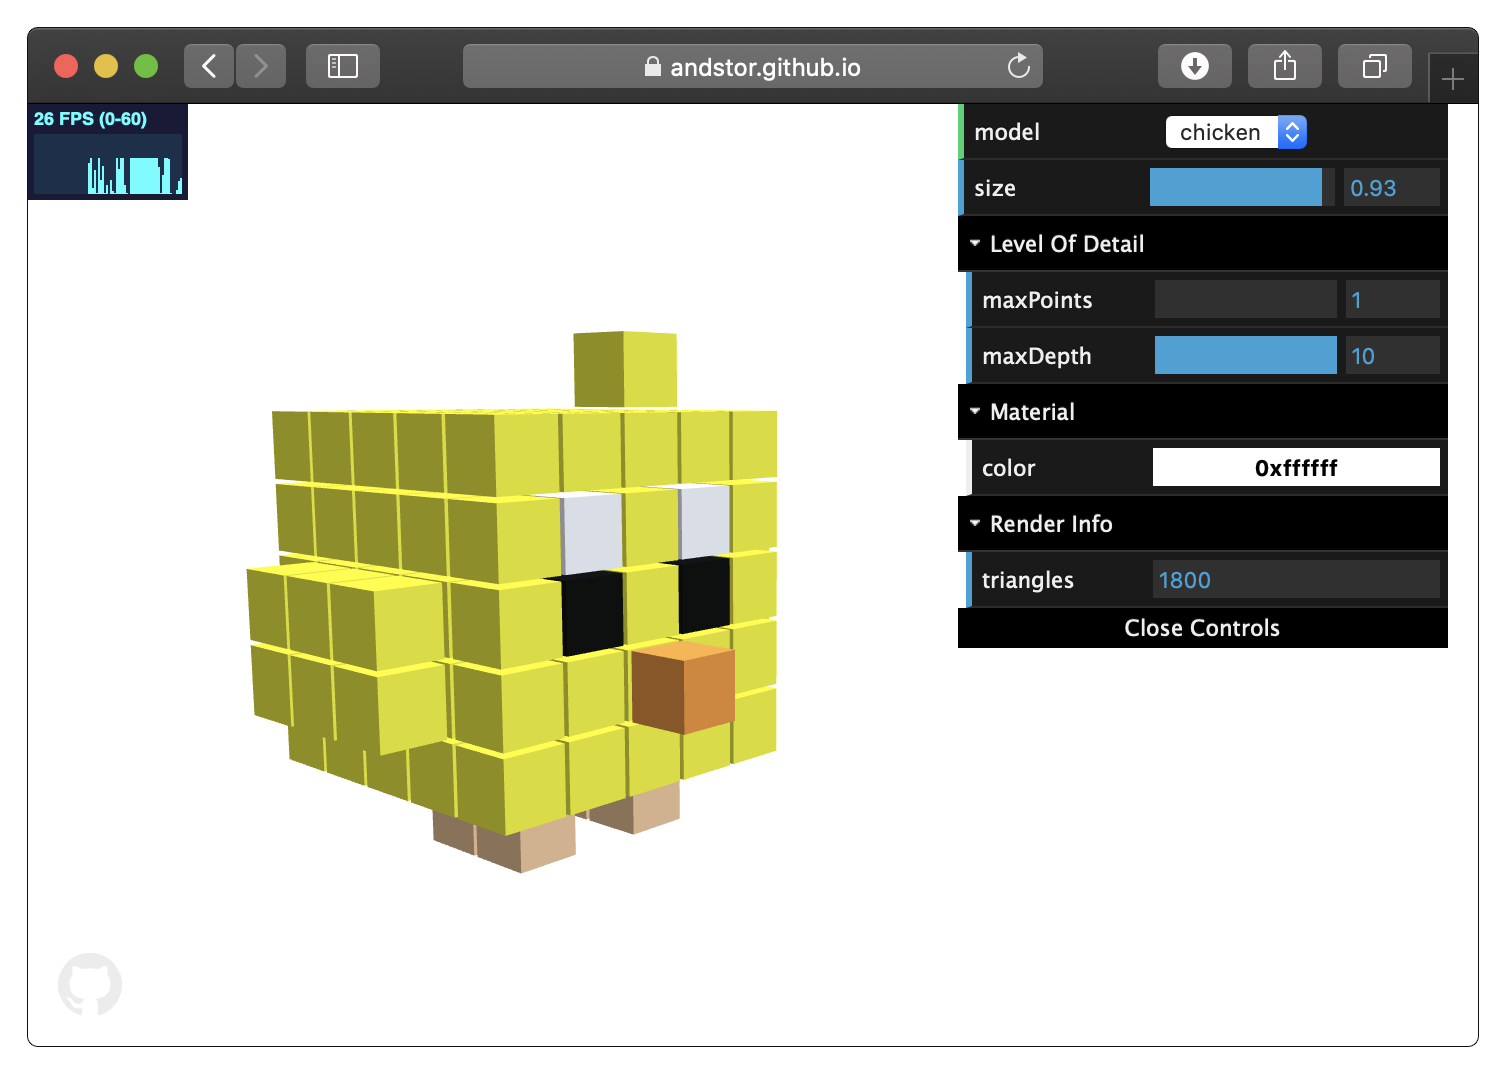
\includegraphics[width=0.9\textwidth]{sections/result/figures/three-voxel-loader-example.png}
    \caption{Screenshot of the three-voxel-loader example page at GitHub Pages.}
    \label{fig:three-voxel-loader-example}
\end{figure}

\section{Voxelizer}
The new Voxelizer engine version v1.0.0 is greatly improved, compared to the old version v0.1.3. The engine is completly redesigned, and resolves all known problems and bugs the old engine had. Further, several new features are implemented, making the engine even more powerfull. Among the new features are support for coloring and shell voxelization, in addition to several new exporting formats. The performance of the engine is also drastically improved. Other improvements includes both code quality and documentation. In order to provide the engine with an own identity, a new logo for the engine is created, as shown in Figure~\ref{fig:voxelizer-logo}.
\begin{figure}[htp]
    \centering
    
\includegraphics[width=0.5\textwidth]{sections/result/figures/voxelizer-logo.eps}
    \caption{Logo for the Voxelizer engine v1.0.0.}
    \label{fig:voxelizer-logo}
\end{figure}

The new version is published to the npm registry, still under the name "voxelizer". The source code is available at GitHub under "andstor/voxelizer". Here, the old version is also available, tagged with the tag "v0.1.3".

\subsection{Voxelization}
The new version of the Vexelizer engine is greatly improved. The engine captures a lot more deatils of the 3D models. It is much more stabile, and produces a lot more consistent results. The engine also provides several new voxelization features. This includes both shell voxelization, and coloring support. Figure~\ref{fig:anvil-render} shows a rendered image of an anvil 3D model developed for testing purposes. The anvil has a blue-ish metallic surface, with several red/gold rust spots. Figure~\ref{fig:result-anvil-voxelization} shows a colored voxelization of this 3D model at a resolution of $2^7$. The individual rust spots are clearly seen, and the overall result seems to be correlating with the original 3D model. Further, in order to showcase the shell voxelization, the voxelization result is cut in half. This is seen in Figure~\ref{fig:result-anvil-voxelization-cut}.
\begin{figure}[htp]
    \centering
    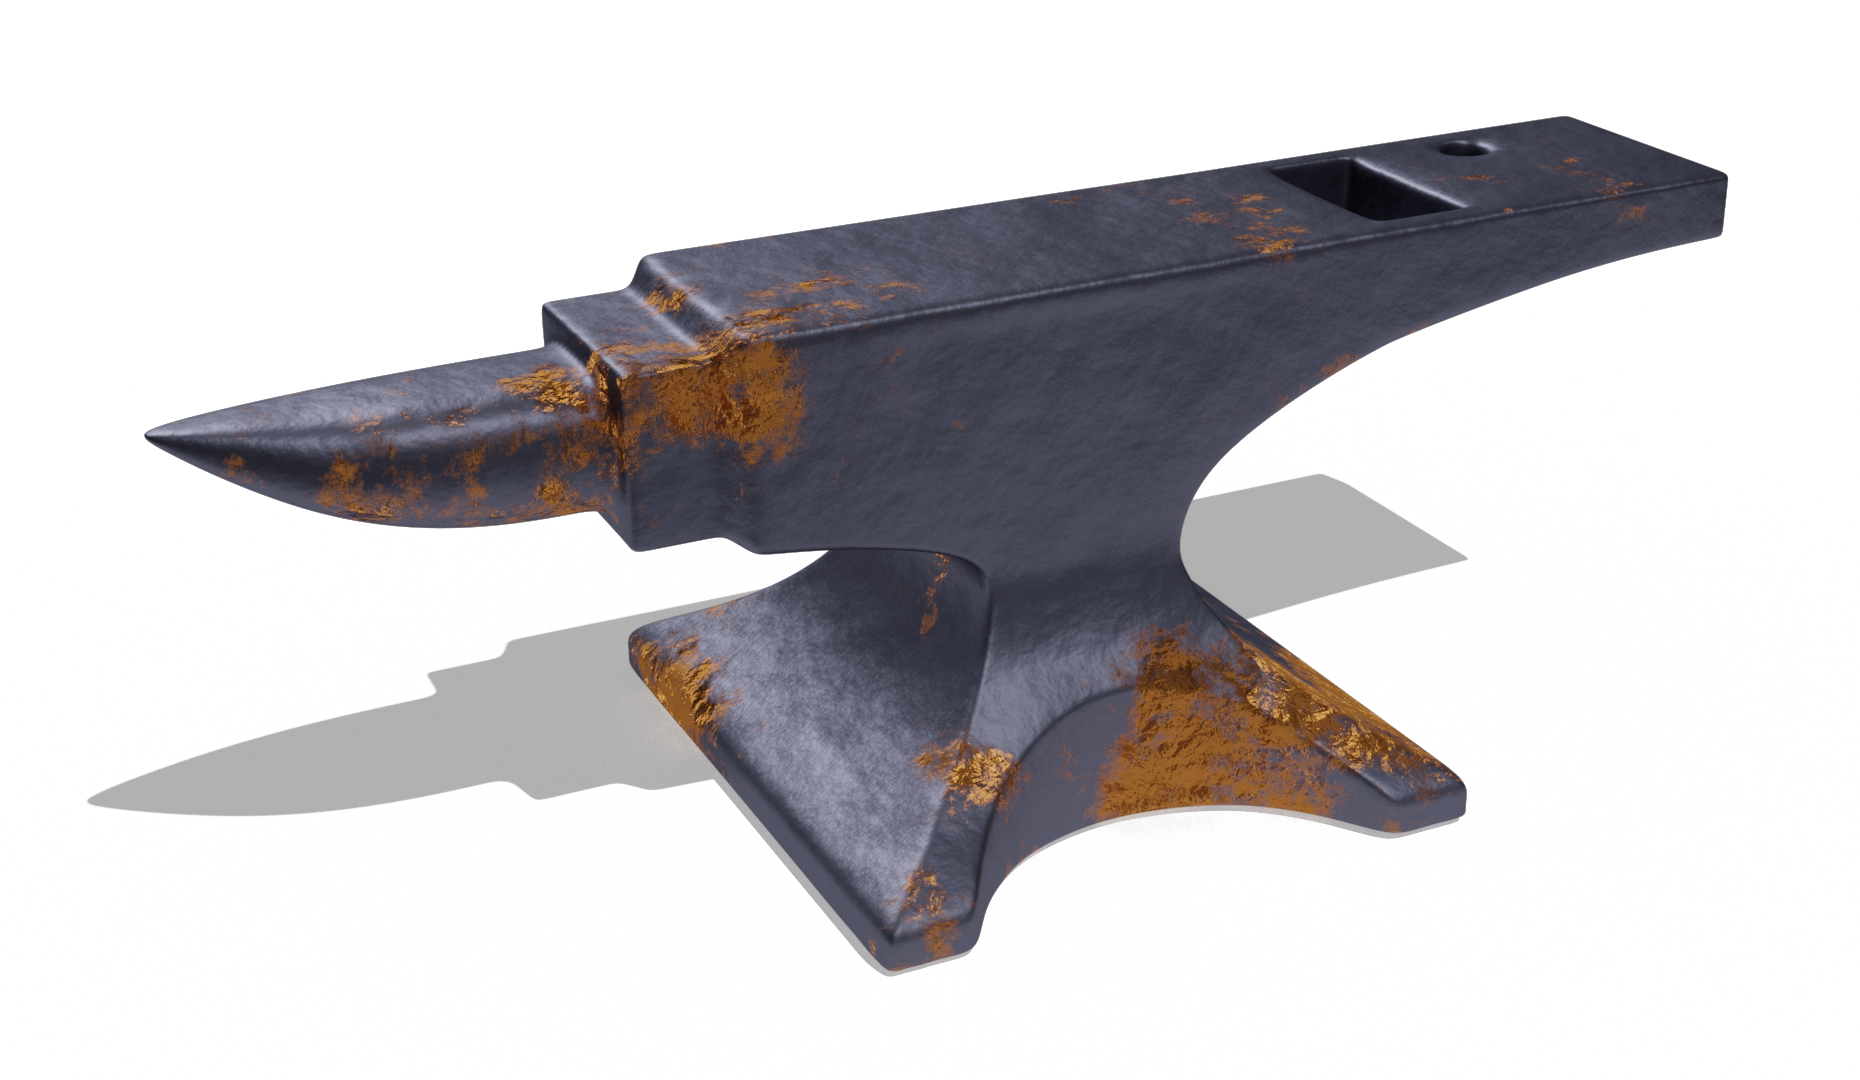
\includegraphics[width=0.95\textwidth]{sections/result/figures/anvil-color-render.png}
    \caption{Render of anvil 3D model.}
    \label{fig:anvil-render}
\end{figure}
\begin{figure}[htp]
    \centering
    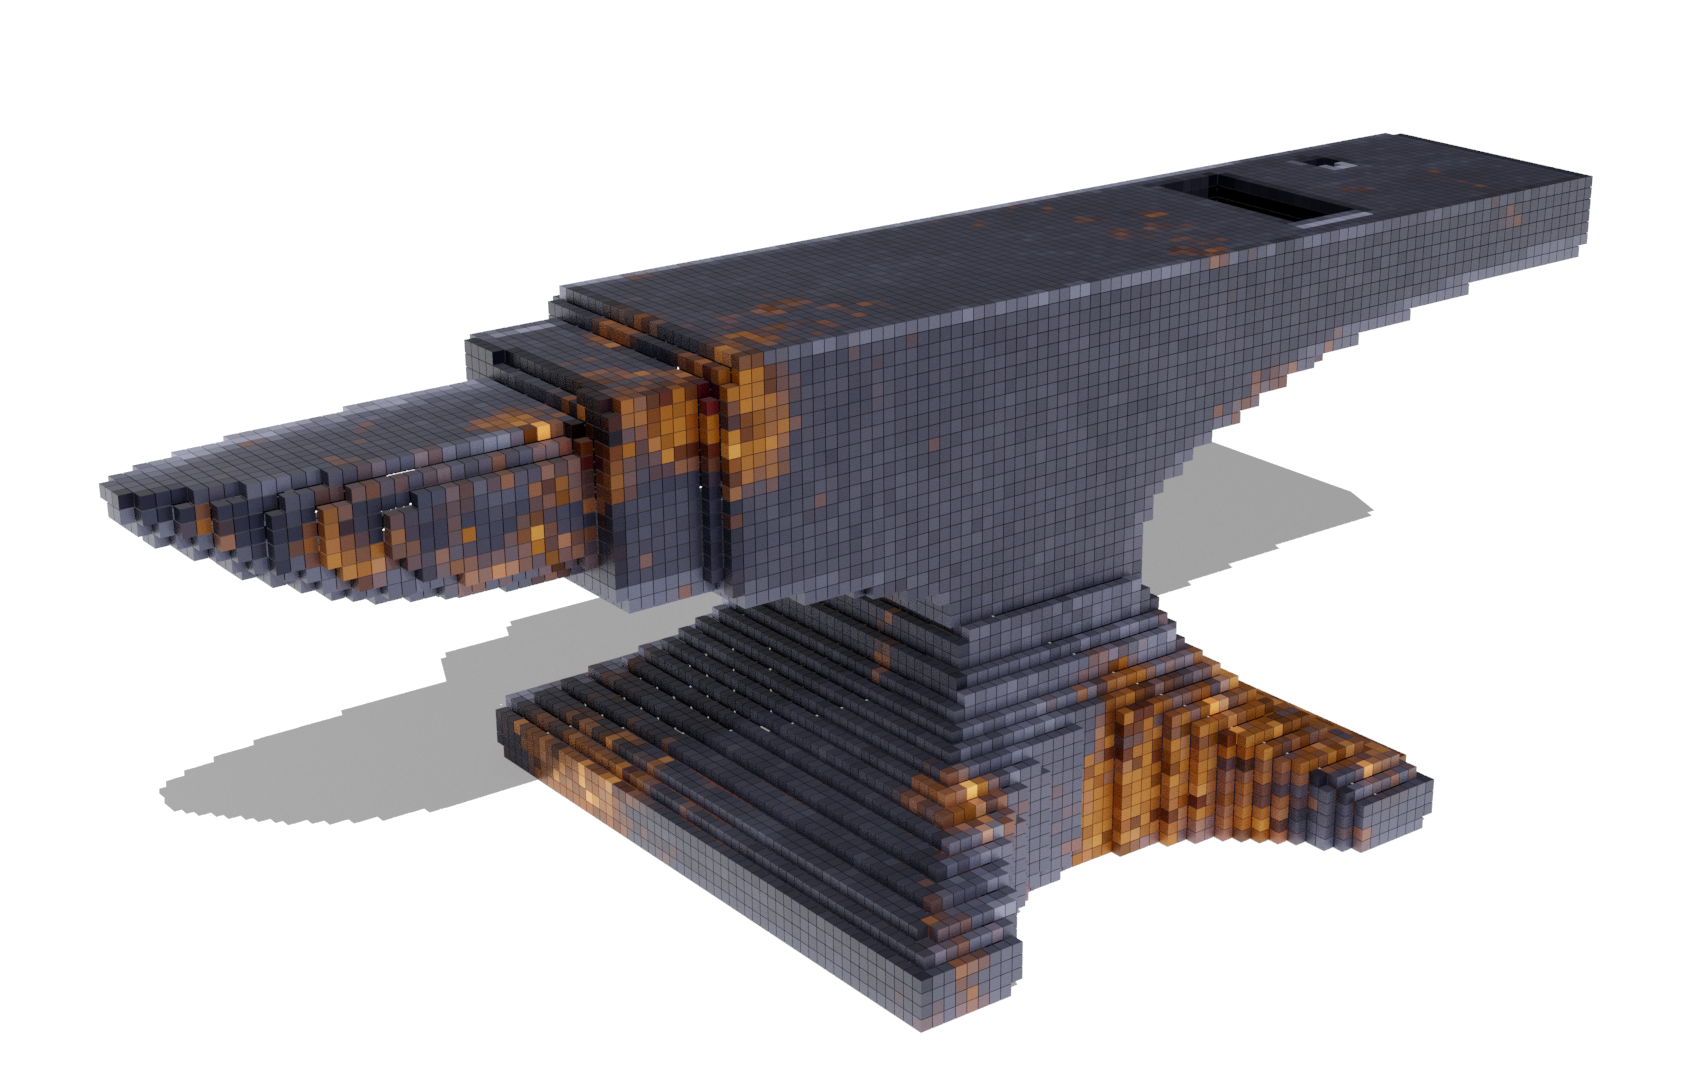
\includegraphics[width=0.95\textwidth]{sections/result/figures/anvil-voxelized-v1-color-128.png}
    \caption{Render of anvil 3D model.}
    \label{fig:result-anvil-voxelization}
\end{figure}
\begin{figure}[htp]
    \centering
    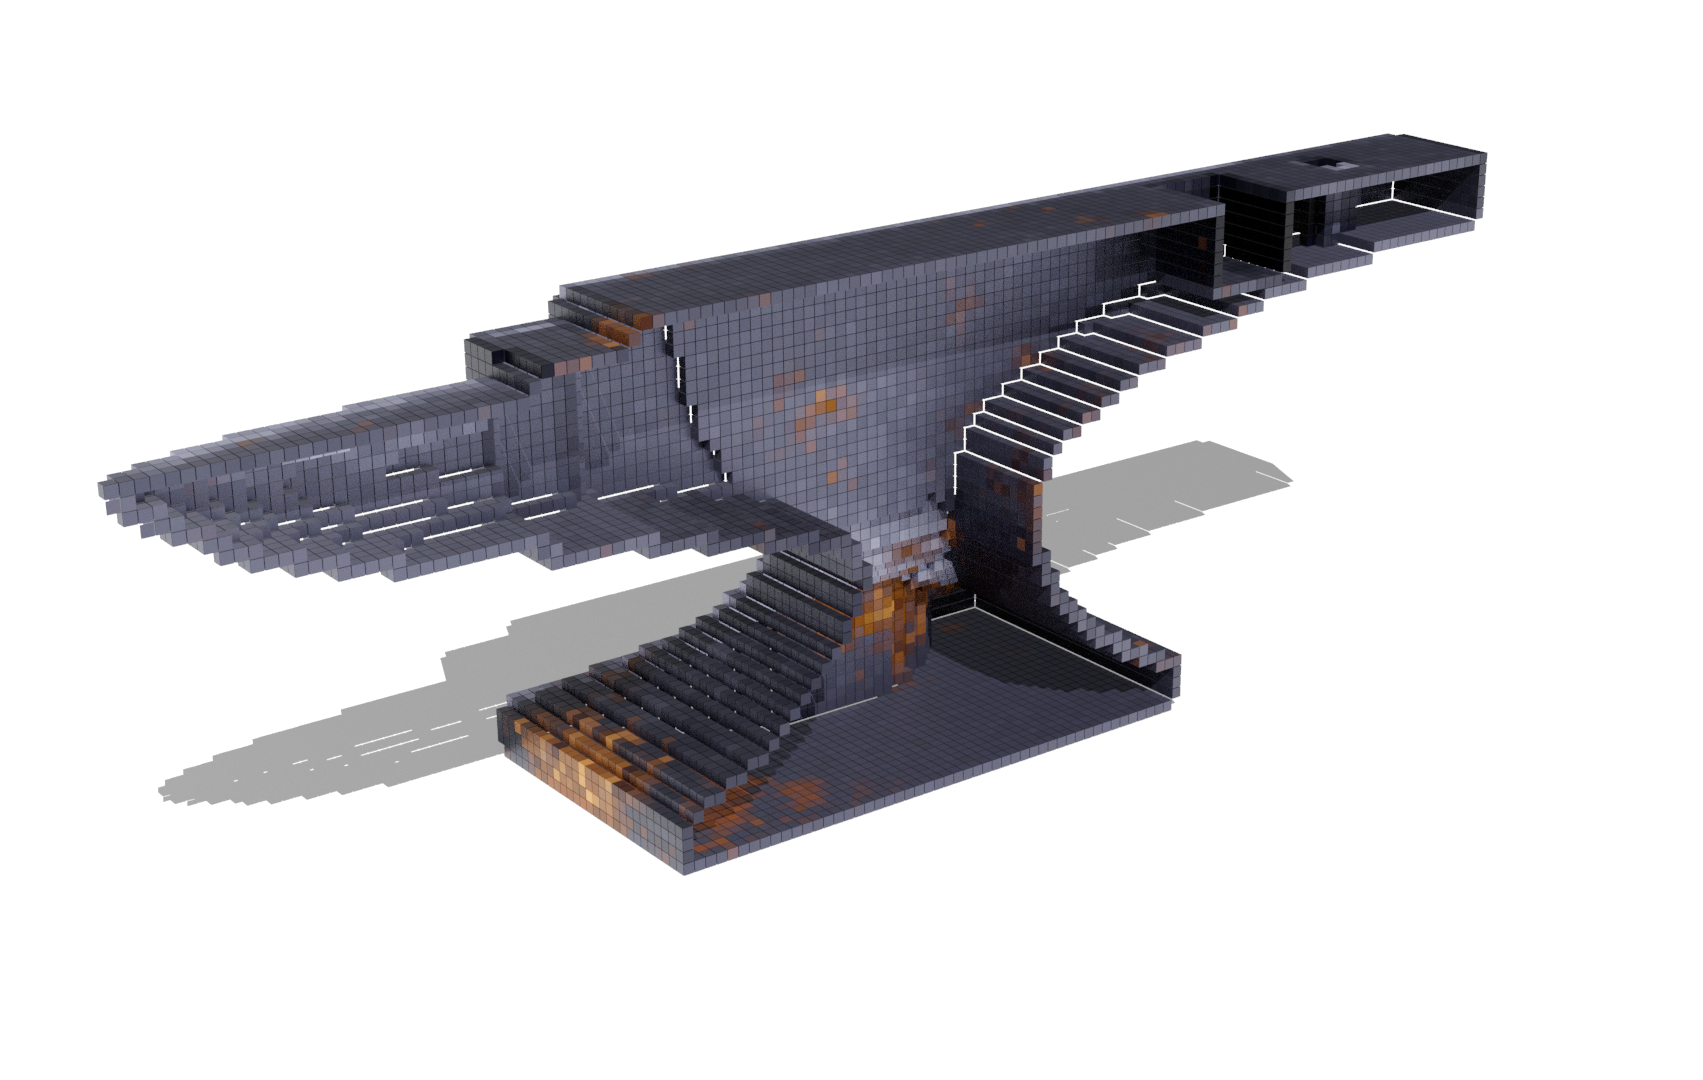
\includegraphics[width=0.95\textwidth]{sections/result/figures/anvil-voxelized-clipped-v1-color-128.png}
    \caption{Render of anvil 3D model.}
    \label{fig:result-anvil-voxelization-cut}
\end{figure}

\clearpage
\subsection{Visual assesment}
In this section, the various improvements of the problems the old engine had will be presented. Fistly, the old engine produced a lot of artifacts. The new version fixes this problem. This can be seen in Figure~\ref{fig:result-voxelizer-comparison-monkey}, which shows the voxelization of a monkey 3D model. Figure~\ref{fig:result-voxelizer-v0.1.3-monkey} shows the voxelization of a monkey with the old version, and Figure~\ref{fig:result-voxelizer-v1-monkey} shows the result with the new version. Comparing the two, it is clear that the new engine produces voxelizations where the artifacts are more or less completly removed.
\begin{figure}[htp]
    \centering
    \begin{subfigure}[b]{0.49\textwidth}
        \centering
        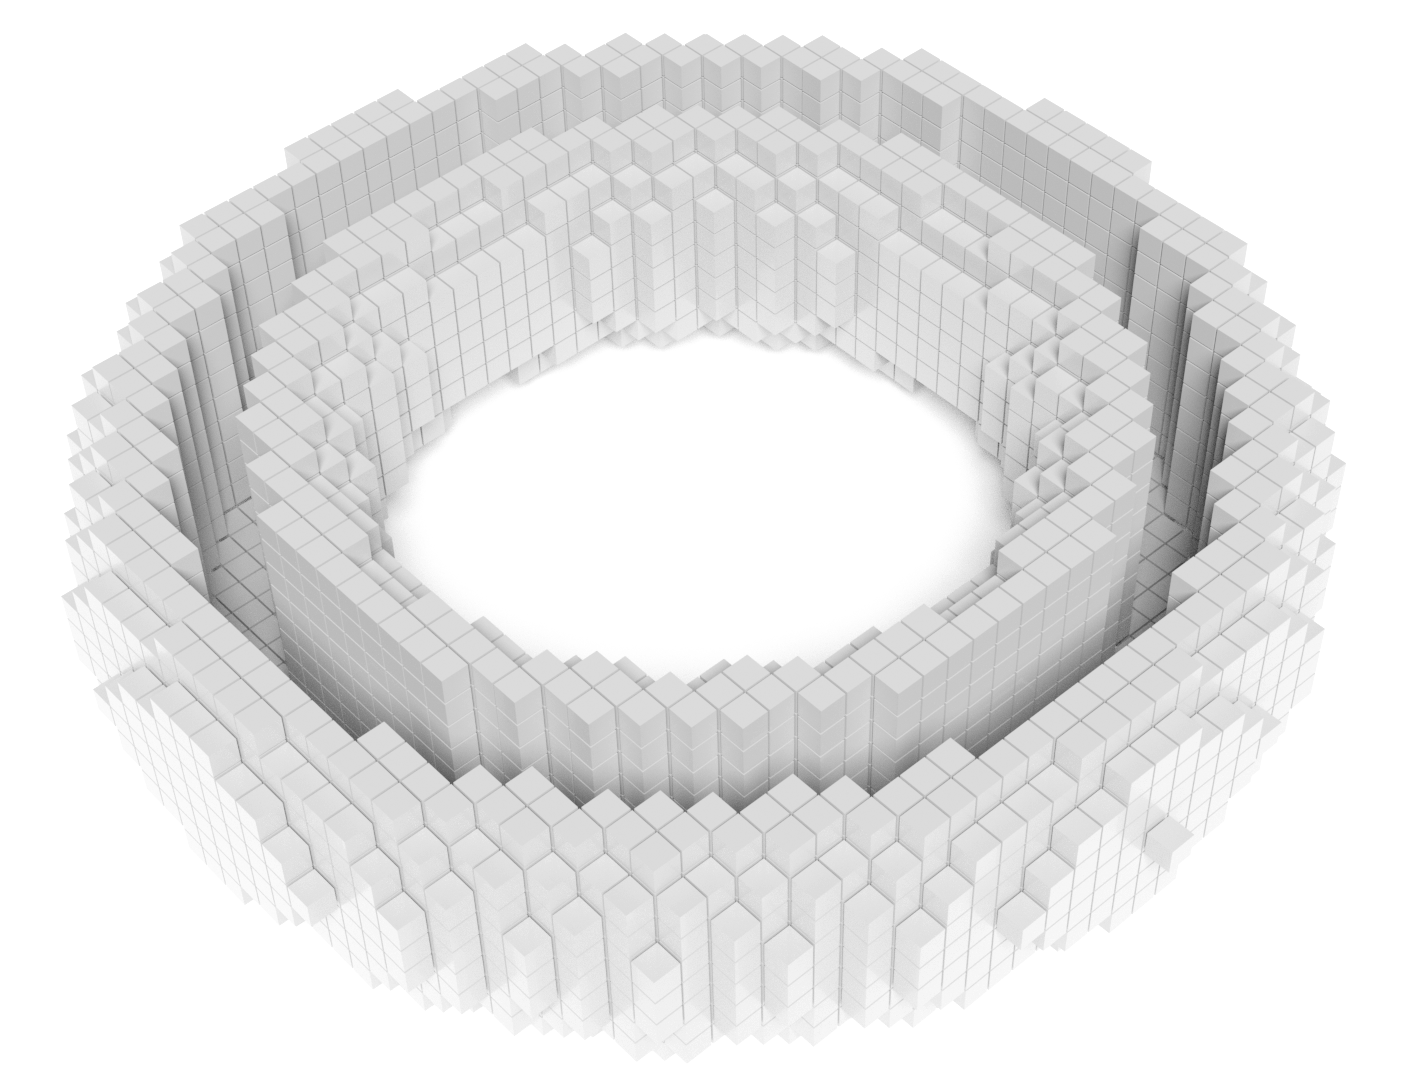
\includegraphics[width=\textwidth]{sections/theory/figures/voxelizer-v013-torus-40.png}
        \caption{Voxelized torus with Voxelizer v0.1.3.}
        \label{fig:result-voxelizer-v0.1.3-torus}
    \end{subfigure}
    \hfill
    \begin{subfigure}[b]{0.49\textwidth}
        \centering
        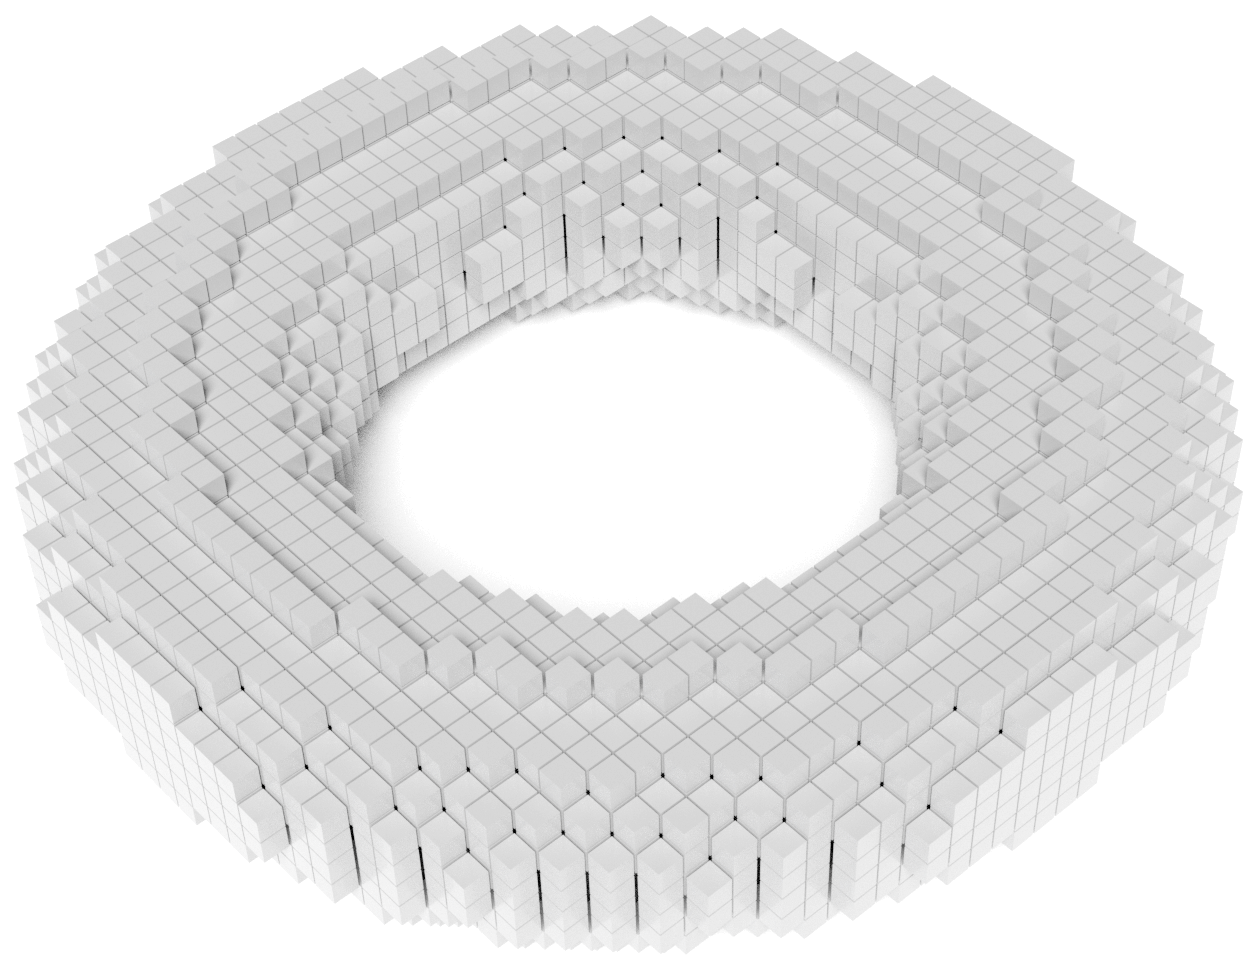
\includegraphics[width=\textwidth]{sections/result/figures/torus-voxelized-v1-40.png}
        \caption{Voxelized torus with Voxelizer v1.0.0.}
        \label{fig:result-voxelizer-v1-torus}
    \end{subfigure}
    \par\bigskip
    \begin{subfigure}[b]{0.49\textwidth}
        \centering
        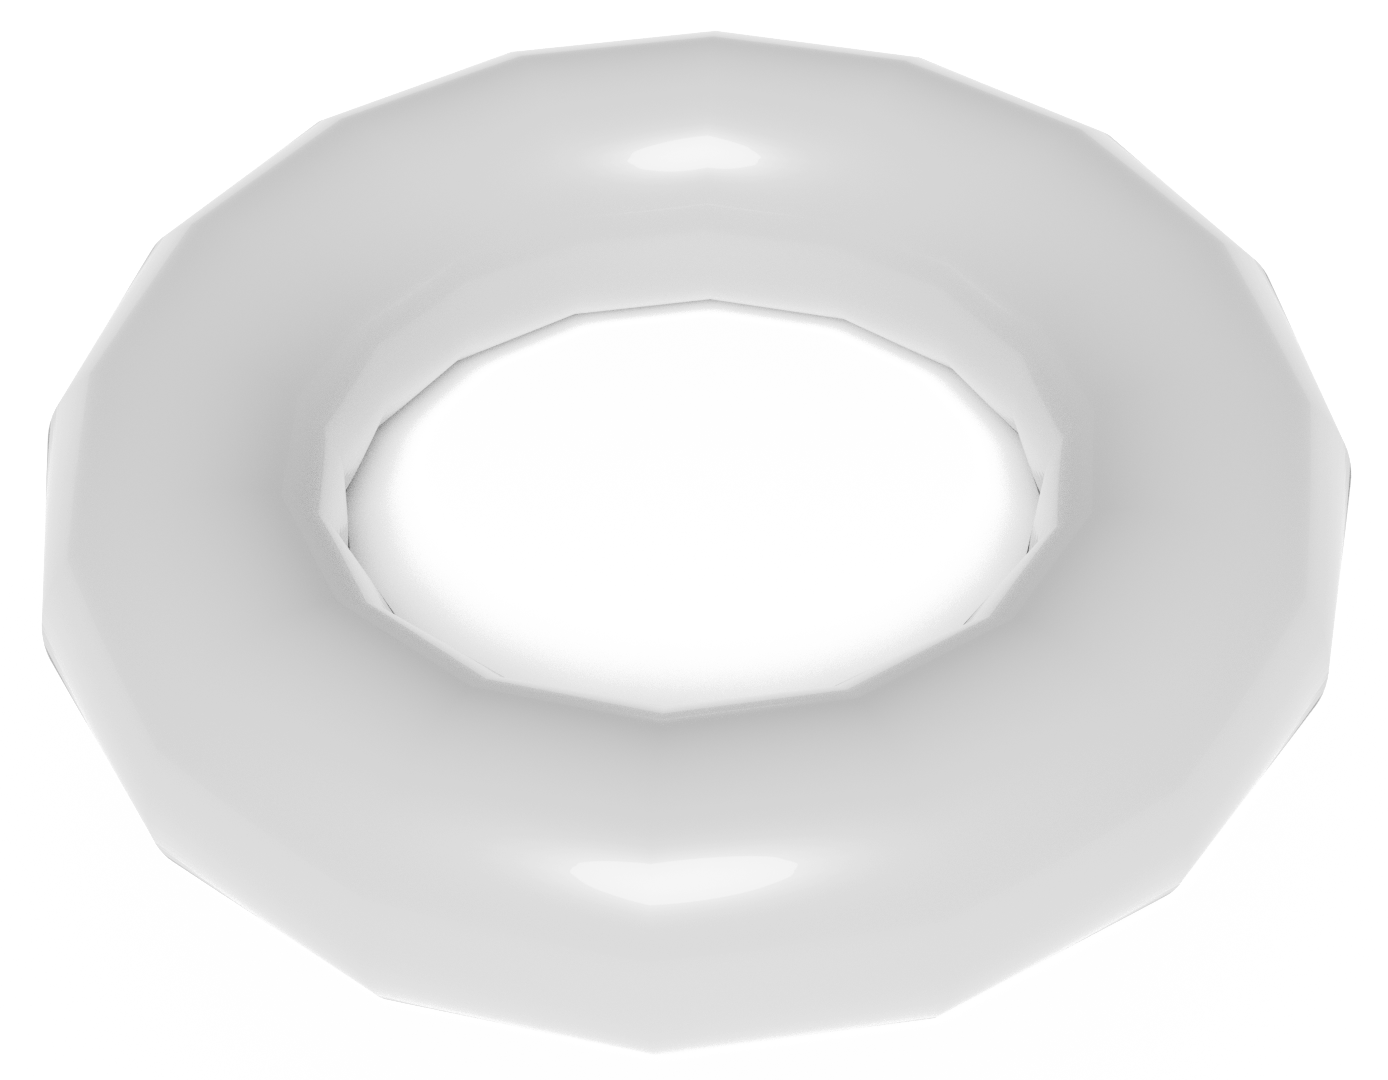
\includegraphics[width=\textwidth]{sections/theory/figures/torus.png}
        \caption{Original torus 3D model.}
        \label{fig:result-original-torus}
    \end{subfigure}
    \caption{Voxelization of a torus with Voxelizer v0.1.3 and v1.0.0. The voxelization is done with a resolution of 40.}
    \label{fig:result-voxelizer-comparison-torus}
\end{figure}
\clearpage
As mentioned in Section~\ref{sec:voxelizer-v013}, the old engine produced a lot of artifacts. The new version fixes this problem. This can be seen in Figure~\ref{fig:result-voxelizer-comparison-monkey}, which shows the voxelization of a monkey 3D model. Figure~\ref{fig:result-voxelizer-v0.1.3-monkey} shows the voxelization of a monkey with the old version, and Figure~\ref{fig:result-voxelizer-v1-monkey} shows the result with the new version. Comparing the two, it is clear that the new engine produces voxelizations where the artifacts are more or less completly removed.
\begin{figure}[hp]
    \centering
    \begin{subfigure}[b]{0.48\textwidth}
        \centering
        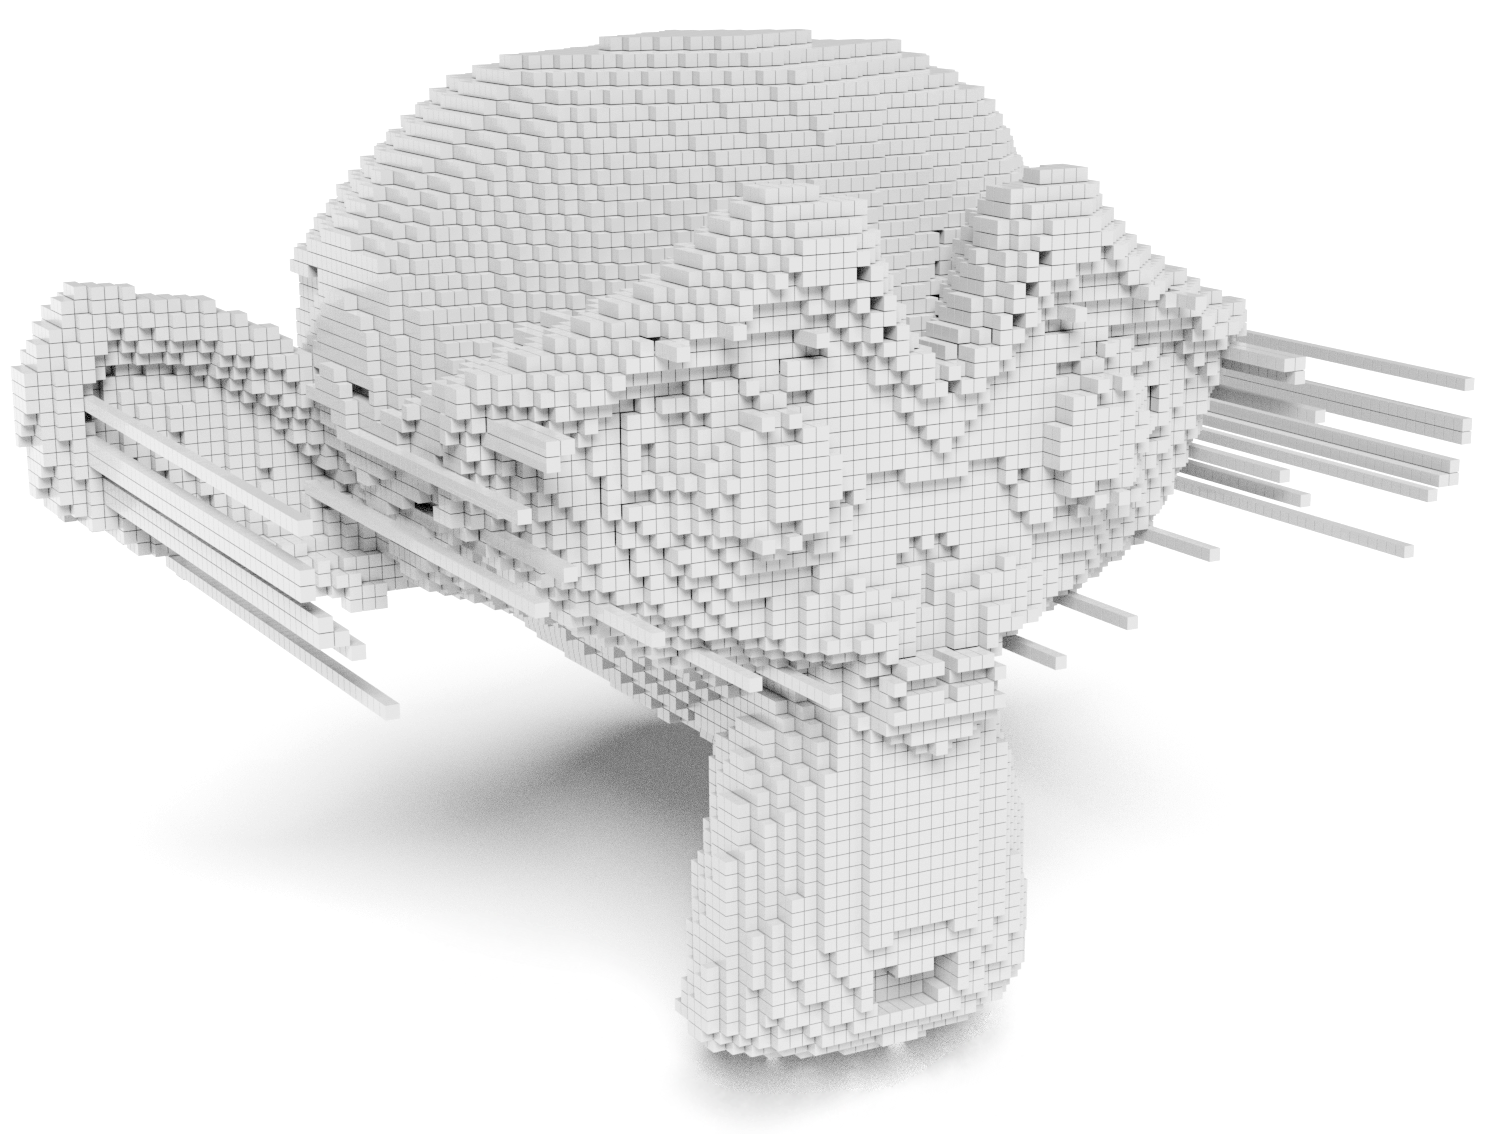
\includegraphics[width=\textwidth]{sections/theory/figures/voxelizer-v013-monkey-100.png}
        \caption{Voxelized monkey with Voxelizer v0.1.3.}
        \label{fig:result-voxelizer-v0.1.3-monkey}
    \end{subfigure}
    \hfill
    \begin{subfigure}[b]{0.50\textwidth}
        \centering
        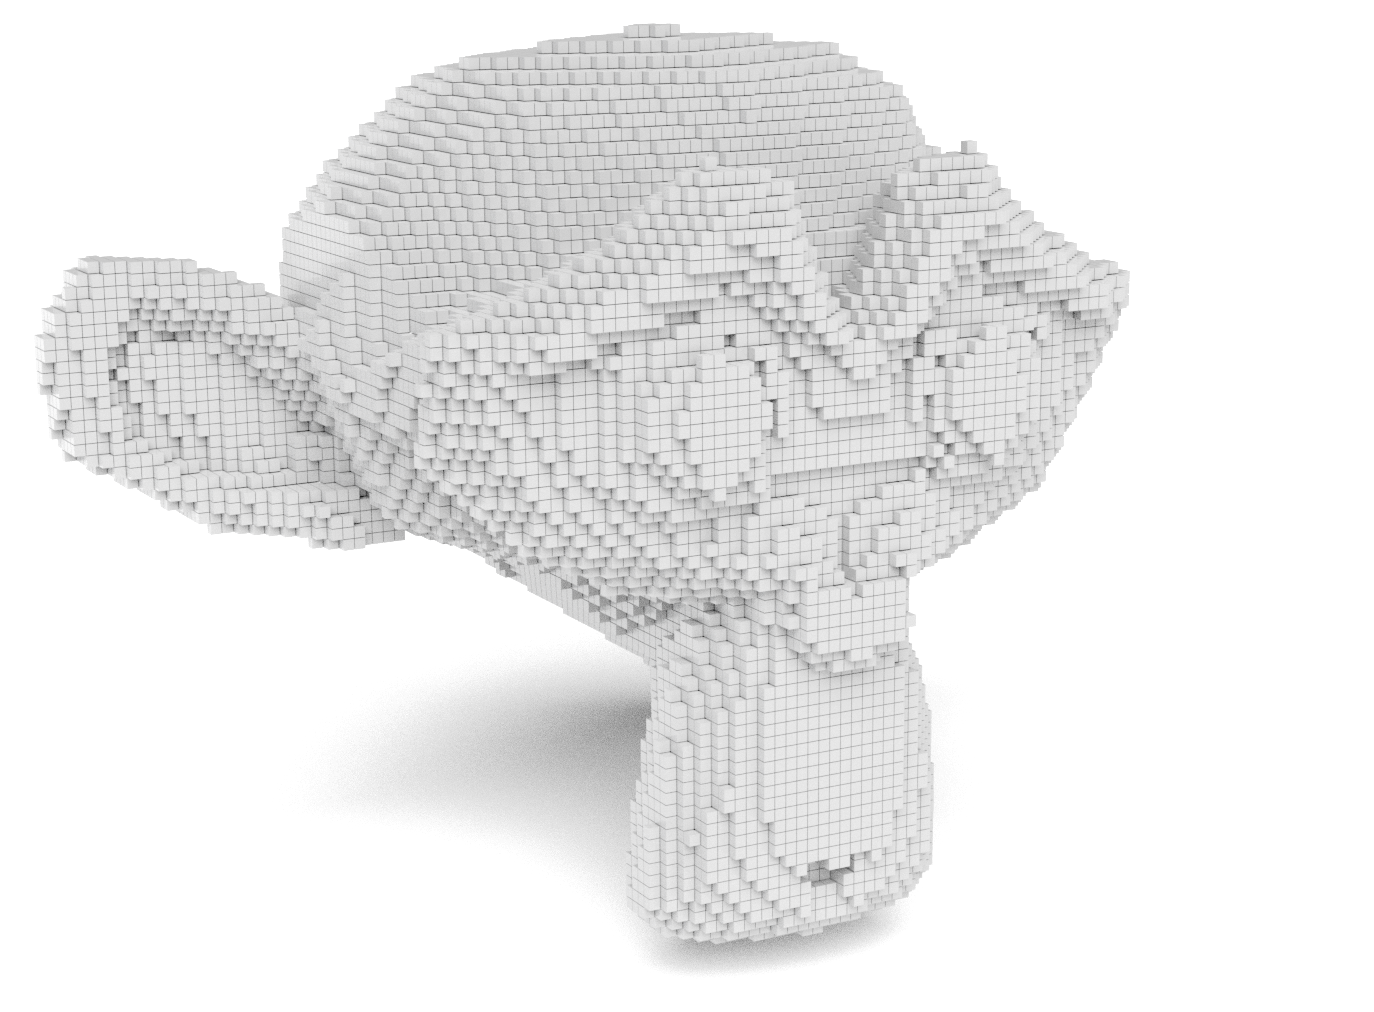
\includegraphics[width=\textwidth]{sections/result/figures/monkey-voxelized-v1-100.png}
        \caption{Voxelized monkey with Voxelizer v1.0.0.}
        \label{fig:result-voxelizer-v1-monkey}
    \end{subfigure}
    \par\bigskip
    \begin{subfigure}[b]{0.43\textwidth}
        \centering
        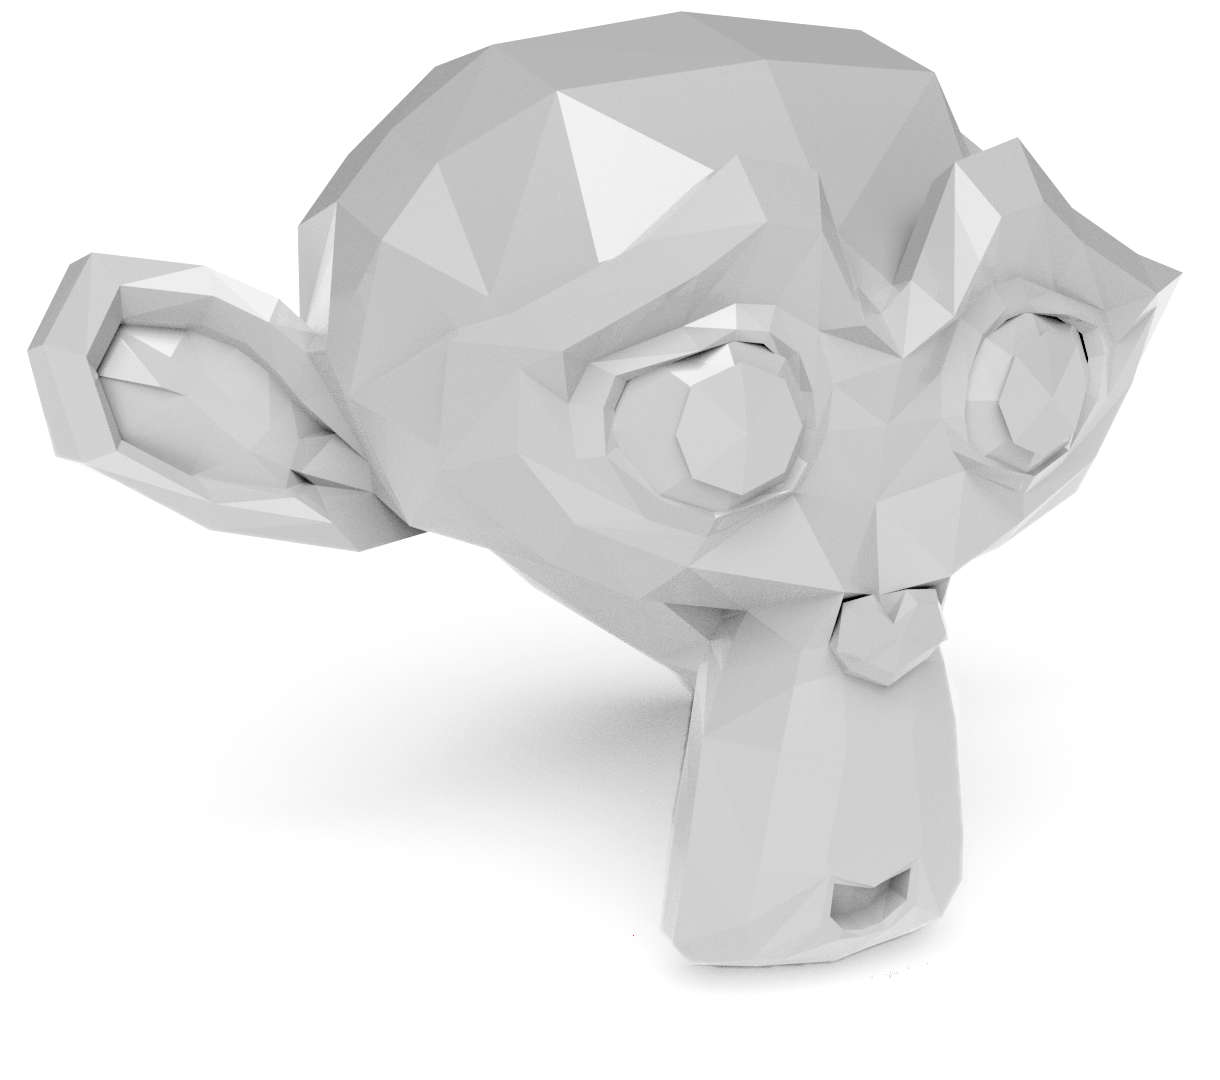
\includegraphics[width=\textwidth]{sections/theory/figures/monkey.png}
        \caption{Original monkey 3D model.}
        \label{fig:result-original-monkey}
    \end{subfigure}
    \hfill
    \caption{Voxelization of a monkey with Voxelizer v0.1.3 and v1.0.0. The voxelization is done with a resolution of 100.}
    \label{fig:result-voxelizer-comparison-monkey}
\end{figure}
\clearpage
The voxelization with the old engine often fails in filling in the gap between the sampled front and back. This produces a completly unusable result. Also, since it is only sampled from the front and back, the details from the other sides of the models are not captured in the voxelization. The new version is much more robust, and captures details from all six sides of the model. This results in a much more accurate representation of the model. This improvement can clearly be seen in Figure~\ref{fig:result-voxelizer-comparison-anvil}, which shows the voxelization of an anvil 3D model. Figure~\ref{fig:result-voxelizer-v0.1.3-anvil} shows a voxelization of an anvil with the old engine. Here, the voxelization has failed in the filling process. Figure~\ref{fig:result-voxelizer-v1-anvil} shows the result with the new version. Comparing the two, it is clear that the new engine produces a lot more accureate voxelizations.
\begin{figure}[hp!]
    \centering
    \begin{subfigure}[b]{0.7\textwidth}
        \centering
        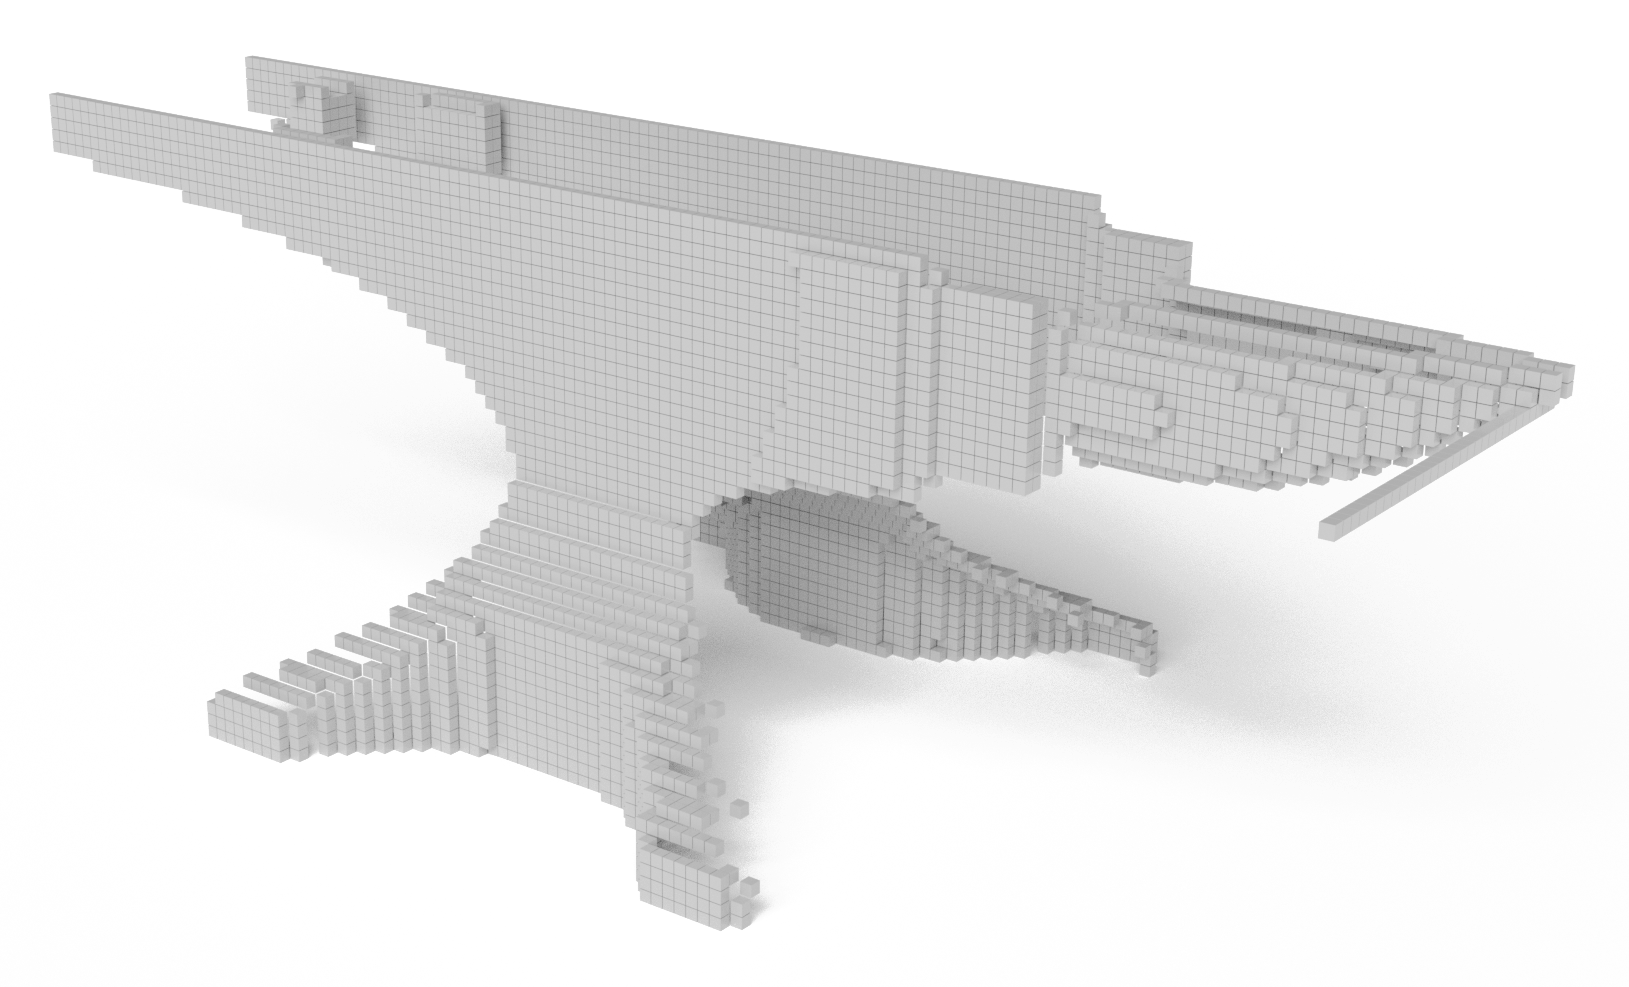
\includegraphics[width=\textwidth]{sections/theory/figures/voxelizer-v013-anvil-128.png}
        \caption{Voxelized anvil with Voxelizer v0.1.3.}
        \label{fig:result-voxelizer-v0.1.3-anvil}
    \end{subfigure}
    \\
    \begin{subfigure}[b]{0.7\textwidth}
        \centering
        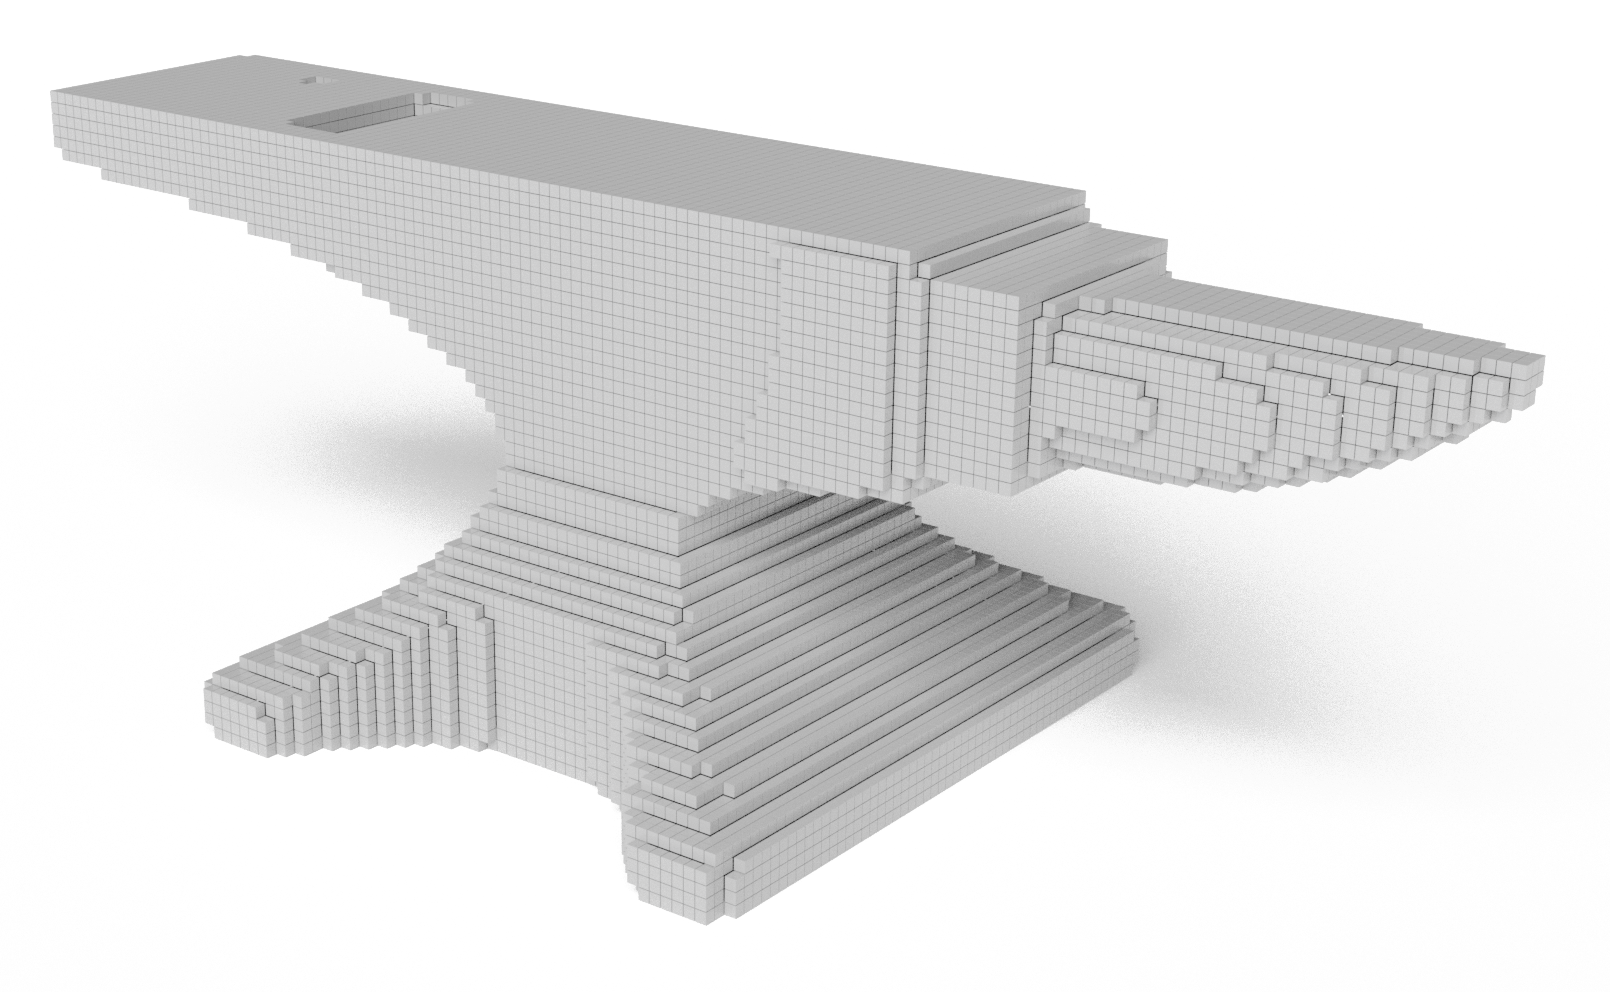
\includegraphics[width=\textwidth]{sections/result/figures/anvil-voxelized-v1-128.png}
        \caption{Voxelized anvil with Voxelizer v1.0.0.}
        \label{fig:result-voxelizer-v1-anvil}
    \end{subfigure}
    \\
    \begin{subfigure}[b]{0.7\textwidth}
        \centering
        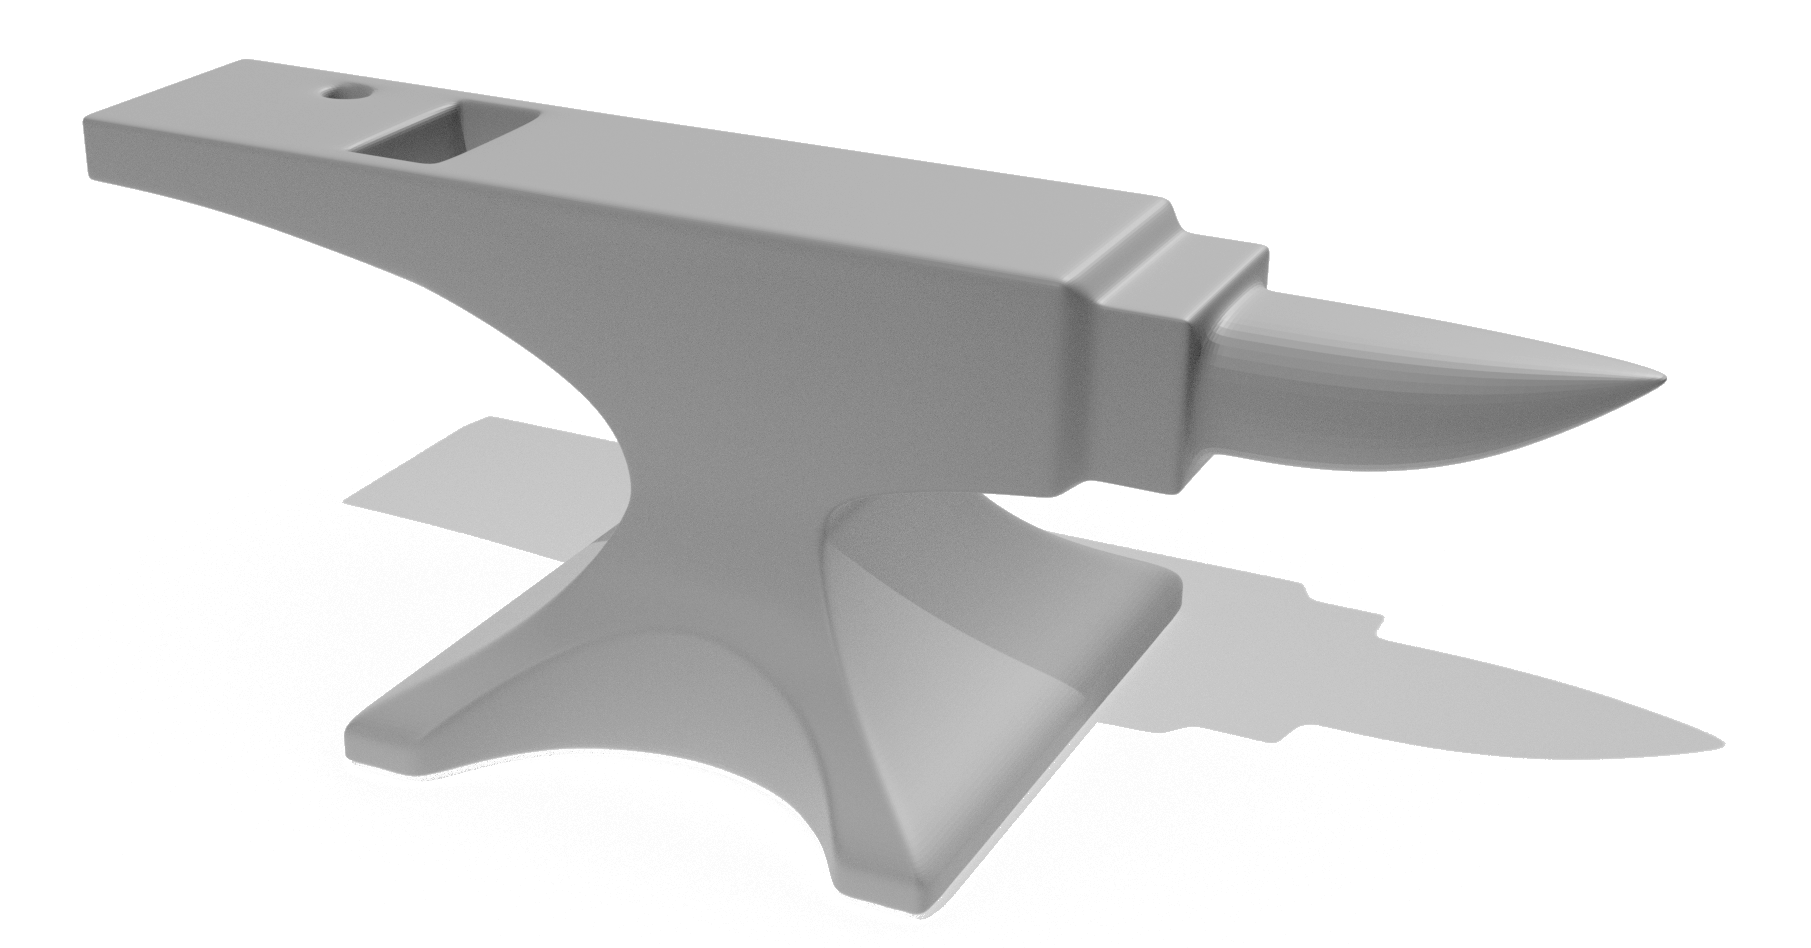
\includegraphics[width=\textwidth]{sections/theory/figures/anvil.png}
        \caption{Original anvil 3D model.}
        \label{fig:result-original-anvil}
    \end{subfigure}
    \hfill
    \caption{Voxelization of a monkey with Voxelizer v0.1.3 and v1.0.0. The voxelization is done with a resolution of $2^7$.}
    \label{fig:result-voxelizer-comparison-anvil}
\end{figure}
\clearpage
\subsection{Performance}
The engine's algorithm is completly overhault. The old raycasting algorithm has a time complexity of:
\[ \mathcal{O}(n^3\times m) \]
where $n$ is the number resolution of the voxelization, and $m$ is the number of triangles in the 3D model. In order to produce and more accurate result, the new algorithm does a lot more sampling. Despite this, the time complexity is redused. With the settings set to colorless and filled, the time complexity of the upgraded raycasting algorithm is:
\[ \mathcal{O}(n^3\times \log(m)) \]
where $n$ is the number resolution of the voxelization, and $m$ is the number of triangles in the 3D model.

Following is a speed and memory comparison of the old and new vesion of the Voxelizer engine. The tests are executed in Node.js v12.16.3. The hardware used is a MacBook Pro (13-inch, 2018) with a 2.3GHz quad core processor and 16GB of 2133MHz LPDDR3 RAM, running MacOS Catalina v10.15.4.

First, the versions are tested with a low-poly mesh. Then, a high-poly mesh is used. The engine is tested at various resolutions. Note that a resolution of $2$ results in $2\times2\times2$ voxels. The old engine version is only able to do a colorless, filled voxelization. In order to make a fair comparison, the new Version's RaycastAlgorithm is set to be colorless and filled. As input, the mesh will be programatically generated by the code provided in Listing~\ref{lst:voxelizer-speed-test-mesh}. This produces a torus mesh with 3200 triangles.
\begin{lstlisting}[language=JavaScript,caption={JS code for generating low-detailed torus mesh.},label={lst:voxelizer-speed-test-mesh}]
    let geometry = new THREE.TorusBufferGeometry( 10, 3, 16, 100 );
    let material = new THREE.MeshBasicMaterial();
    let torus = new THREE.Mesh(geometry, material);
\end{lstlisting}

\clearpage
\begin{figure}[H]
    \centering
    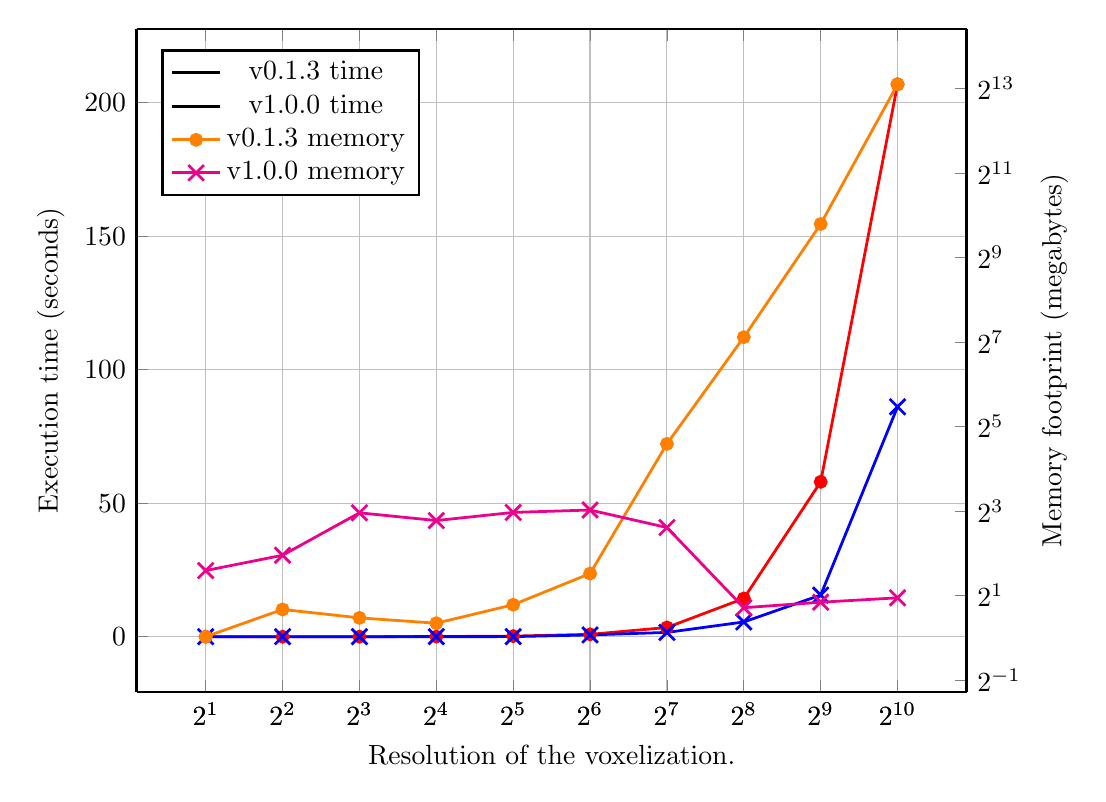
\begin{tikzpicture}
        \begin{semilogxaxis}[
            axis y line*=left,
            xlabel = Resolution of the voxelization.,
            ylabel = Execution time (seconds),
            grid=both,
            log basis x=2,
            width=\textwidth,
            height=10cm,
            ylabel near ticks,
            line width=1pt,
        ]
        \addplot[red,mark=*] coordinates {
            (2^1,  0.0254)
            (2^2,  0.0116)
            (2^3,  0.0195)
            (2^4,  0.0624)
            (2^5,  0.2288)
            (2^6,  0.8879)
            (2^7,  3.4578)
            (2^8,  14.3298)
            (2^9,  58.0136)
            (2^10, 206.8811)
        };\label{TimeOldPlot}
        \addplot[blue,mark=x,mark size=4] coordinates {
            (2^1, 0.0154)
            (2^2, 0.0172)
            (2^3, 0.0214)
            (2^4, 0.0382)
            (2^5, 0.0403)
            (2^6, 0.6752)
            (2^7, 1.6094)
            (2^8, 5.5269)
            (2^9, 15.5968)
            (2^10, 86.0982)
        };\label{TimeNewPlot}
        \end{semilogxaxis}
        \begin{loglogaxis}[
            axis y line*=right,
            ylabel = Memory footprint (megabytes),
            log basis x=2,
            log basis y=2,
            width=\textwidth,
            height=10cm,
            ylabel near ticks,
            line width=1pt,
            legend pos=north west
        ]
        \addlegendimage{/pgfplots/refstyle=TimeOldPlot}\addlegendentry{v0.1.3 time}
        \addlegendimage{/pgfplots/refstyle=TimeNewPlot}\addlegendentry{v1.0.0 time}
        \addplot[orange,mark=*] coordinates {
            (2^1,  1.0146)
            (2^2,  1.5868)
            (2^3,  1.3817)
            (2^4,  1.2659)
            (2^5,  1.7142)
            (2^6,  2.8593)
            (2^7,  24.0315)
            (2^8,  138.2336)
            (2^9,  885.5446)
            (2^10, 8764.2631)
        };\addlegendentry{v0.1.3 memory}
        \addplot[magenta,mark=x,mark size=4] coordinates {
            (2^1,  3.00344)
            (2^2,  3.8611)
            (2^3,  7.7465)
            (2^4,  6.8227)
            (2^5,  7.7983)
            (2^6,  8.1104)
            (2^7,  6.0841)
            (2^8,  1.6326)
            (2^9,  1.7861)
            (2^10, 1.9199)
        };\addlegendentry{v1.0.0 memory}
        \end{loglogaxis}
    \end{tikzpicture}
    \caption{Plot over execution time and memory footprint for voxelization of a low-detailed mesh with the old and new Voxelizer engine.}
    \label{fig:plot-execution-time-low-poly}
\end{figure}
\begin{table}[H]
    \newcolumntype{Y}{>{\centering\arraybackslash}X}
    \begin{minipage}[t]{.45\linewidth}
        \centering
        \caption{Execution times and memory footprints for voxelization of low-detailed mesh with Voxelizer v0.1.3}
        \label{tab:performance-voxelizer-v0.1.3-low-poly}
        \medskip
        \begin{tabularx}{\textwidth}{*{3}{|Y}|}
            \hline
            \textbf{Resolution}& \textbf{Time (sec)} & \textbf{Memory (MB)}\\
            \hline
            2\textsuperscript{1} & 0.0254 & 1.0146 \\
            2\textsuperscript{2} & 0.0116 & 1.5868 \\
            2\textsuperscript{3} & 0.0195 & 1.3817 \\
            2\textsuperscript{4} & 0.0624 & 1.2659 \\
            2\textsuperscript{5} & 0.2288 & 1.7142 \\
            2\textsuperscript{6} & 0.8879 & 2.8593 \\
            2\textsuperscript{7} & 3.4578 & 24.0315 \\
            2\textsuperscript{8} & 14.3298 & 138.2336 \\
            2\textsuperscript{9} & 58.0136 & 885.5446 \\
            2\textsuperscript{10} & 260.8811 & 8764.2631 \\
            \hline
        \end{tabularx}
    \end{minipage}\hfill
    \begin{minipage}[t]{.45\linewidth}
        \centering
        \caption{Execution times and memory footprints for voxelization of low-detailed mesh with Voxelizer v1.0.0}
        \label{tab:performance-voxelizer-v1.0.0-low-poly}
        \medskip
        \begin{tabularx}{\textwidth}{*{3}{|Y}|}
            \hline
            \textbf{Resolution} & \textbf{Time (sec)} & \textbf{Memory (MB)}\\
            \hline
            2\textsuperscript{1} & 0.0154 & 3.00344\\
            2\textsuperscript{2} & 0.0172 & 3.8611\\
            2\textsuperscript{3} & 0.0214 & 7.7465\\
            2\textsuperscript{4} & 0.0382 & 6.8227\\
            2\textsuperscript{5} & 0.0403 & 7.7983\\
            2\textsuperscript{6} & 0.6752 & 8.1104\\
            2\textsuperscript{7} & 1.6094 & 6.0841\\
            2\textsuperscript{8} & 5.5269 & 1.6326\\
            2\textsuperscript{9} & 15.5968 & 1.7861\\
            2\textsuperscript{10} & 86.0982 & 1.9199\\
            \hline
        \end{tabularx}
    \end{minipage}
\end{table}

Figure~\ref{fig:plot-execution-time-low-poly} shows a graph over the execution time and the memory footprint for a voxelization of a low-detailed mesh with the Voxelizer engine v0.1.3 and v1.0.0. The raw data is available in Table~\ref{tab:performance-voxelizer-v0.1.3-low-poly} and Table~\ref{tab:performance-voxelizer-v1.0.0-low-poly}.

The new engine has a relatively low memory footprint. At resolutions from $2^1$ to $2^7$, the memory consumption stays around 7MB. Then, at a resolution of $2^8$, the memory drops to around 2MB. This is most likely due to the JavaScript Garbage Collector (GC) kicking in. At larger resolutions, the memory seems to stay relatively stabile around 2MB. The old engine starts with a very low memory footprint. It stays low, between 1MB and 2MB, from a resolution of $2^1$ to $2^6$. Then, the memory footprint starts to increase rapidly. A total of 24MB are used for a resolution of $2^7$. At $2^10$ the footprint has risen to 8.7GB. This is most likely due to the fact that the old engine used normal JavaScript arrays that dynamically expands. A lot of obsolete data objects will accumulate, and the GC seems to not be able to handle this well.

Regarding execution time, this is also greatly improved in the new engine version. This is especially noticeable at large resolutions. At a resolution of $2^10$, the old engine use 260 seconds to voxelize the 3D model. The new version only use 86 seconds, a reduction of about $60\%$.

A new mesh is generated with the code in Listing~\ref{lst:voxelizer-speed-test-mesh-high}. This produces a highly detailed torus mesh with 1,000,000 triangles. The are presented in the figures below.

\begin{lstlisting}[language=JavaScript,caption={JS code for generating high-detailed torus mesh.},label={lst:voxelizer-speed-test-mesh-high}]
let geometry = new THREE.TorusBufferGeometry( 10, 3, 1000, 500 );
let material = new THREE.MeshBasicMaterial();
let torus = new THREE.Mesh(geometry, material);
\end{lstlisting}
\clearpage
\begin{figure}[H]
    \centering
    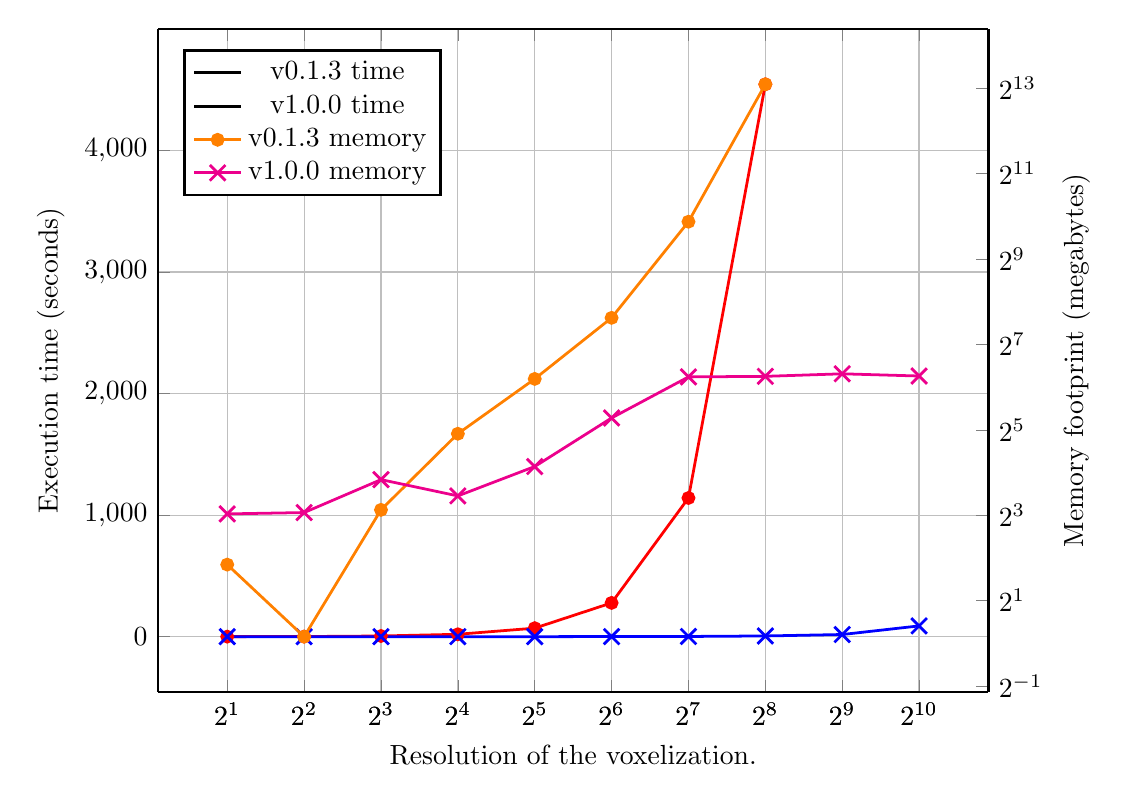
\begin{tikzpicture}
        \begin{semilogxaxis}[
            axis y line*=left,
            xlabel = Resolution of the voxelization.,
            ylabel = Execution time (seconds),
            grid=both,
            log basis x=2,
            width=\textwidth,
            height=10cm,
            ylabel near ticks,
            line width=1pt,
        ]
        \addplot[red,mark=*] coordinates {
            (2^1,  0.5388)
            (2^2,  1.2370)
            (2^3,  5.8674)
            (2^4,  19.8983)
            (2^5,  70.2835)
            (2^6,  278.1215)
            (2^7,  1141.1212)
            (2^8,  4543.6064)
        };\label{TimeOldPlot}
        \addplot[blue,mark=x,mark size=4] coordinates {
            (2^1, 0.17265)
            (2^2, 0.1612)
            (2^3, 0.2277)
            (2^4, 0.2755)
            (2^5, 0.3402)
            (2^6, 1.0793)
            (2^7, 1.9604)
            (2^8, 6.0971)
            (2^9, 17.9376)
            (2^10, 88.8092)
        };\label{TimeNewPlot}
        \end{semilogxaxis}
        \begin{loglogaxis}[
            axis y line*=right,
            ylabel = Memory footprint (megabytes),
            log basis x=2,
            log basis y=2,
            width=\textwidth,
            height=10cm,
            ylabel near ticks,
            line width=1pt,
            legend pos=north west
        ]
        \addlegendimage{/pgfplots/refstyle=TimeOldPlot}\addlegendentry{v0.1.3 time}
        \addlegendimage{/pgfplots/refstyle=TimeNewPlot}\addlegendentry{v1.0.0 time}
        \addplot[orange,mark=*] coordinates {
            (2^1,  3.5880)
            (2^2,  1.1134)
            (2^3,  8.7263)
            (2^4,  30.0106)
            (2^5,  73.1078)
            (2^6,  197.0107 )
            (2^7,  937.7180 )
            (2^8,  8726.9914)
        };\addlegendentry{v0.1.3 memory}
        \addplot[magenta,mark=x,mark size=4] coordinates {
            (2^1,  8.1706)
            (2^2,  8.3496)
            (2^3,  14.2518)
            (2^4,  10.9389)
            (2^5,  17.6270)
            (2^6,  38.7798)
            (2^7,  75.5248)
            (2^8,  76.1971)
            (2^9,  79.4146)
            (2^10, 76.6116)
        };\addlegendentry{v1.0.0 memory}
        \end{loglogaxis}
    \end{tikzpicture}
    \caption{Plot over execution time and memory footprint for voxelization of a high-detailed mesh with the old and new Voxelizer engine.}
    \label{fig:plot-execution-time-high-poly}
\end{figure}
\begin{table}[ht]
    \newcolumntype{Y}{>{\centering\arraybackslash}X}
    \def\arraystretch{1.5}
    \begin{minipage}[t]{.45\linewidth}
        \centering
        \caption{Execution times and memory footprints for voxelization of high-detailed mesh with Voxelizer v0.1.3}
        \label{tab:performance-voxelizer-v0.1.3-high-poly}
        \medskip
        \begin{tabularx}{\textwidth}{*{3}{|Y}|}
            \hline
            \textbf{Resolution}& \textbf{Time (sec)} & \textbf{Memory (MB)}\\
            \hline
            2\textsuperscript{1} & 0.5388 & 3.5880\\
            2\textsuperscript{2} & 1.2370 & 1.1134\\
            2\textsuperscript{3} & 5.8674 & 8.7263\\
            2\textsuperscript{4} & 19.8983 & 30.0106\\
            2\textsuperscript{5} & 70.2835 & 73.1078\\
            2\textsuperscript{6} & 278.1215 & 197.0107 \\
            2\textsuperscript{7} & 1141.1212 & 937.7180 \\
            2\textsuperscript{8} & 4543.6064 & 8726.9914\\
            \hline
        \end{tabularx}
    \end{minipage}\hfill
    \begin{minipage}[t]{.45\linewidth}
        \centering
        \caption{Execution times and memory footprints for voxelization of high-detailed mesh with Voxelizer v1.0.0}
        \label{tab:performance-voxelizer-v1.0.0-high-poly}
        \medskip
        \begin{tabularx}{\textwidth}{*{3}{|Y}|}
            \hline
            \textbf{Resolution} & \textbf{Time (sec)} & \textbf{Memory (MB)}\\
            \hline
            2\textsuperscript{1} & 0.17265 & 8.1706\\
            2\textsuperscript{2} & 0.1612 & 8.3496\\
            2\textsuperscript{3} & 0.2277 & 14.2518\\
            2\textsuperscript{4} & 0.2755 & 10.9389\\
            2\textsuperscript{5} & 0.3402 & 17.6270\\
            2\textsuperscript{6} & 1.0793 & 38.7798\\
            2\textsuperscript{7} & 1.9604 & 75.5248\\
            2\textsuperscript{8} & 6.0971 & 76.1971\\
            2\textsuperscript{9} & 17.9376 & 79.4146\\
            2\textsuperscript{10} & 88.8092 & 76.6116\\
            \hline
        \end{tabularx}
    \end{minipage}
\end{table}

Figure~\ref{fig:plot-execution-time-high-poly} shows a graph over the execution time and the memory footprint for a voxelization of a high-detailed mesh with the Voxelizer engine v0.1.3 and v1.0.0. The raw data is available in Table~\ref{tab:performance-voxelizer-v0.1.3-high-poly} and Table~\ref{tab:performance-voxelizer-v1.0.0-high-poly}.

The results shows similar characteristics as the ones with the low detailed mesh. However, very noticeable is the large difference in execution time. The old version is able to voxelize the mesh with 1,000,000 triangles in 4543 seconds, about 75 minutes. The new version is able to do the same in only about 6.1 second. The new version is also tested at a resolution of $2^10$. This takes only 88.8 seconds. This massive performance improvement is mainly due to the raycasting optimization discussed in Section~\ref{sec:three.js-optimization}.

The memory consumption of the old version is more or less the same as with a low detailed mesh. The new version does consume more memory than in the previous test. This is because the BVH tree generated for the raycasting performance improvement does need a bit of memory. The memory footprint of the new version seems to gradually scale up from 8MB at a resolution of $2^1$, to 76MB at resolution $2^7$. From here on, the memory footprint stay more or less constant. This is because the BVH implementation gradually builds up the BVH tree, as described in Section~\ref{sec:three.js-optimization}.

\subsection{Exporting}
Several formats...
- XML
- BINVOX
- 3D array
- ndarray

\subsection{Code quality}
This section describes how the code quality is improved. The old codebase had several problems. Firstly, all the code was contained in one large file. This made it hard to navigate and the code was messy. The new version makes use of ES Modules, enabling to organize the code in different files. Secondly, the engine previously hardcoded the one algorithm used. The new version includes an easily extensible algorithm system. This is ensured through the use of inheritance and factory patterns, as discussed in Section~\ref{sec:method-algorithm-system}. Thirdly, the code did barely include tests for the system. The new version now includes unit tests for almost the whole engine. Lastly, the code had no code documentation. This is resolved by writing JSDoc for all classes and functions. This documentation is also made easily accessible at GitHub Pages with the help of the new JSDoc Action, presented in Section~\ref{sec:result-jsdoc-action}. A screenshot of the public documentation page is shown in Figure~\ref{fig:result-voxelizer-documentation}.
\begin{figure}[htp]
    \centering
    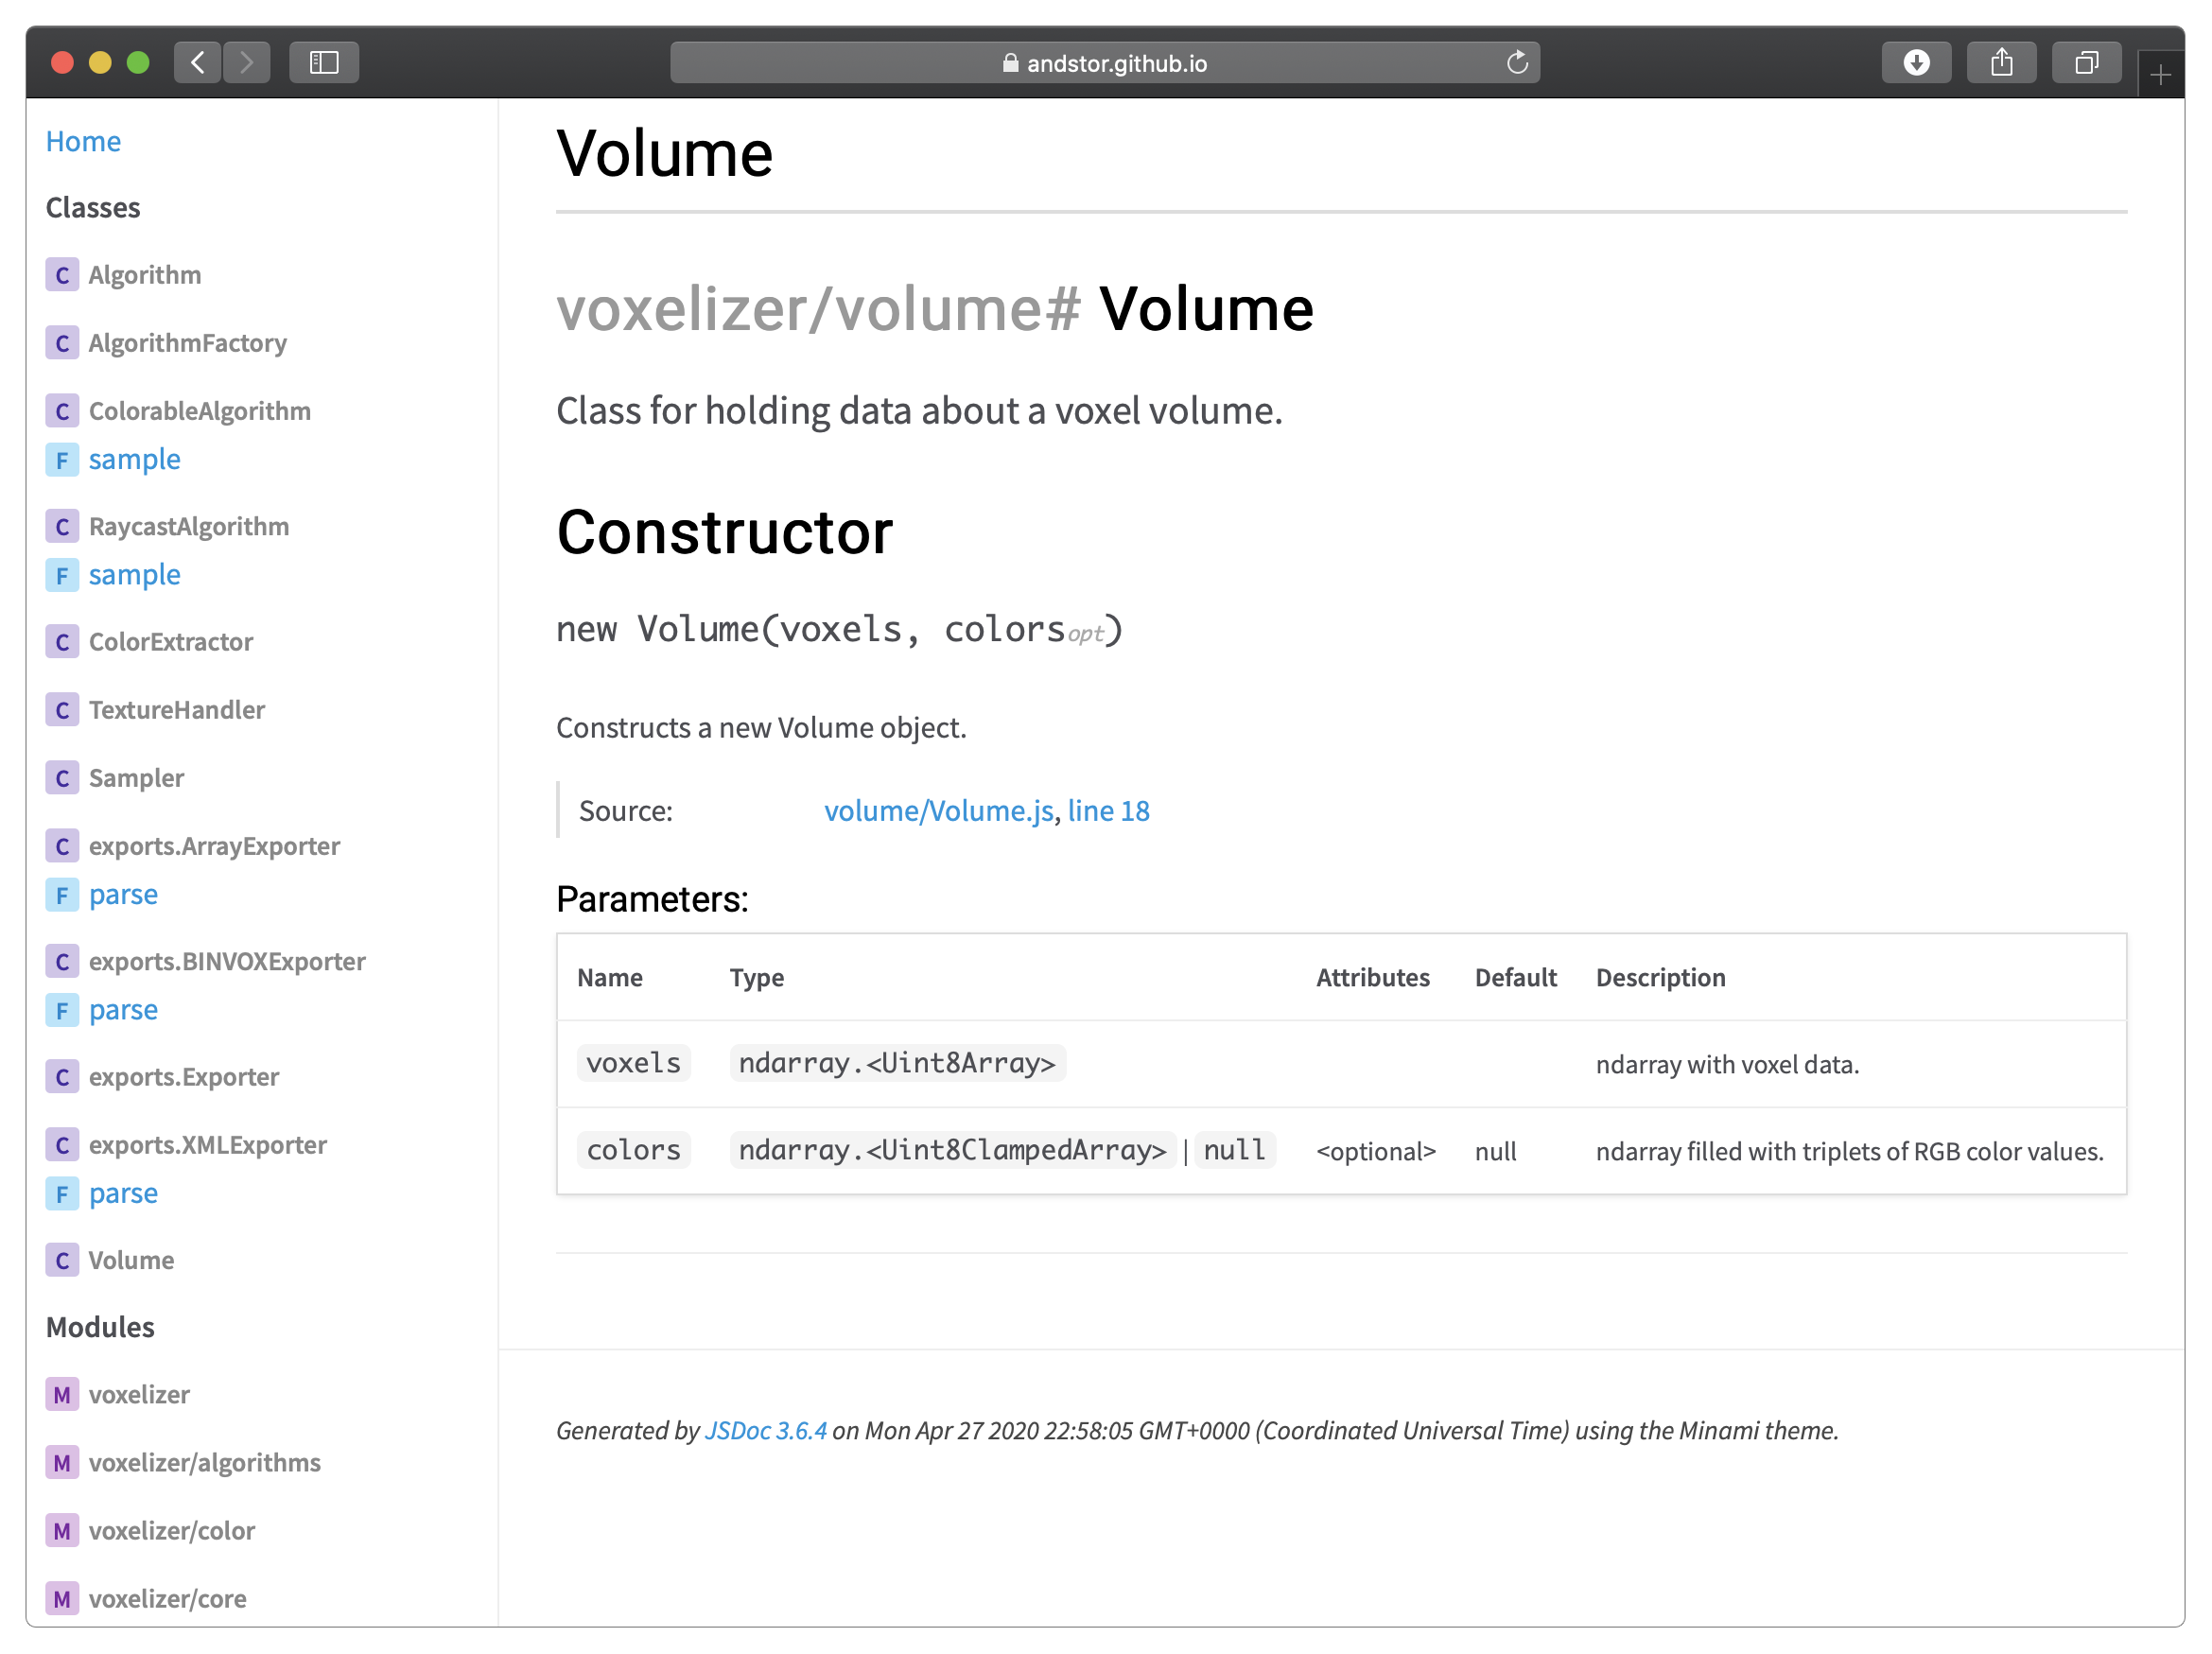
\includegraphics[width=0.9\textwidth]{sections/result/figures/voxelizer-documentation.png}
    \caption{Public documentation for the Voxelizer engine.}
    \label{fig:result-voxelizer-documentation}
\end{figure}

\subsection{Example}
An example of the engine is deployed to GitHub Pages. Visit \url{https://andstor.github.io/voxelizer/examples/} to see the example. Figure~\ref{fig:voxelizer-example} shows a screenshot of the site. The example includes a GUI with controls for controlling, among other things, the resolution, shell or solid voxelization, the LOD, and clipping planes for visually inspecting the results.
\begin{figure}[ht]
    \centering
    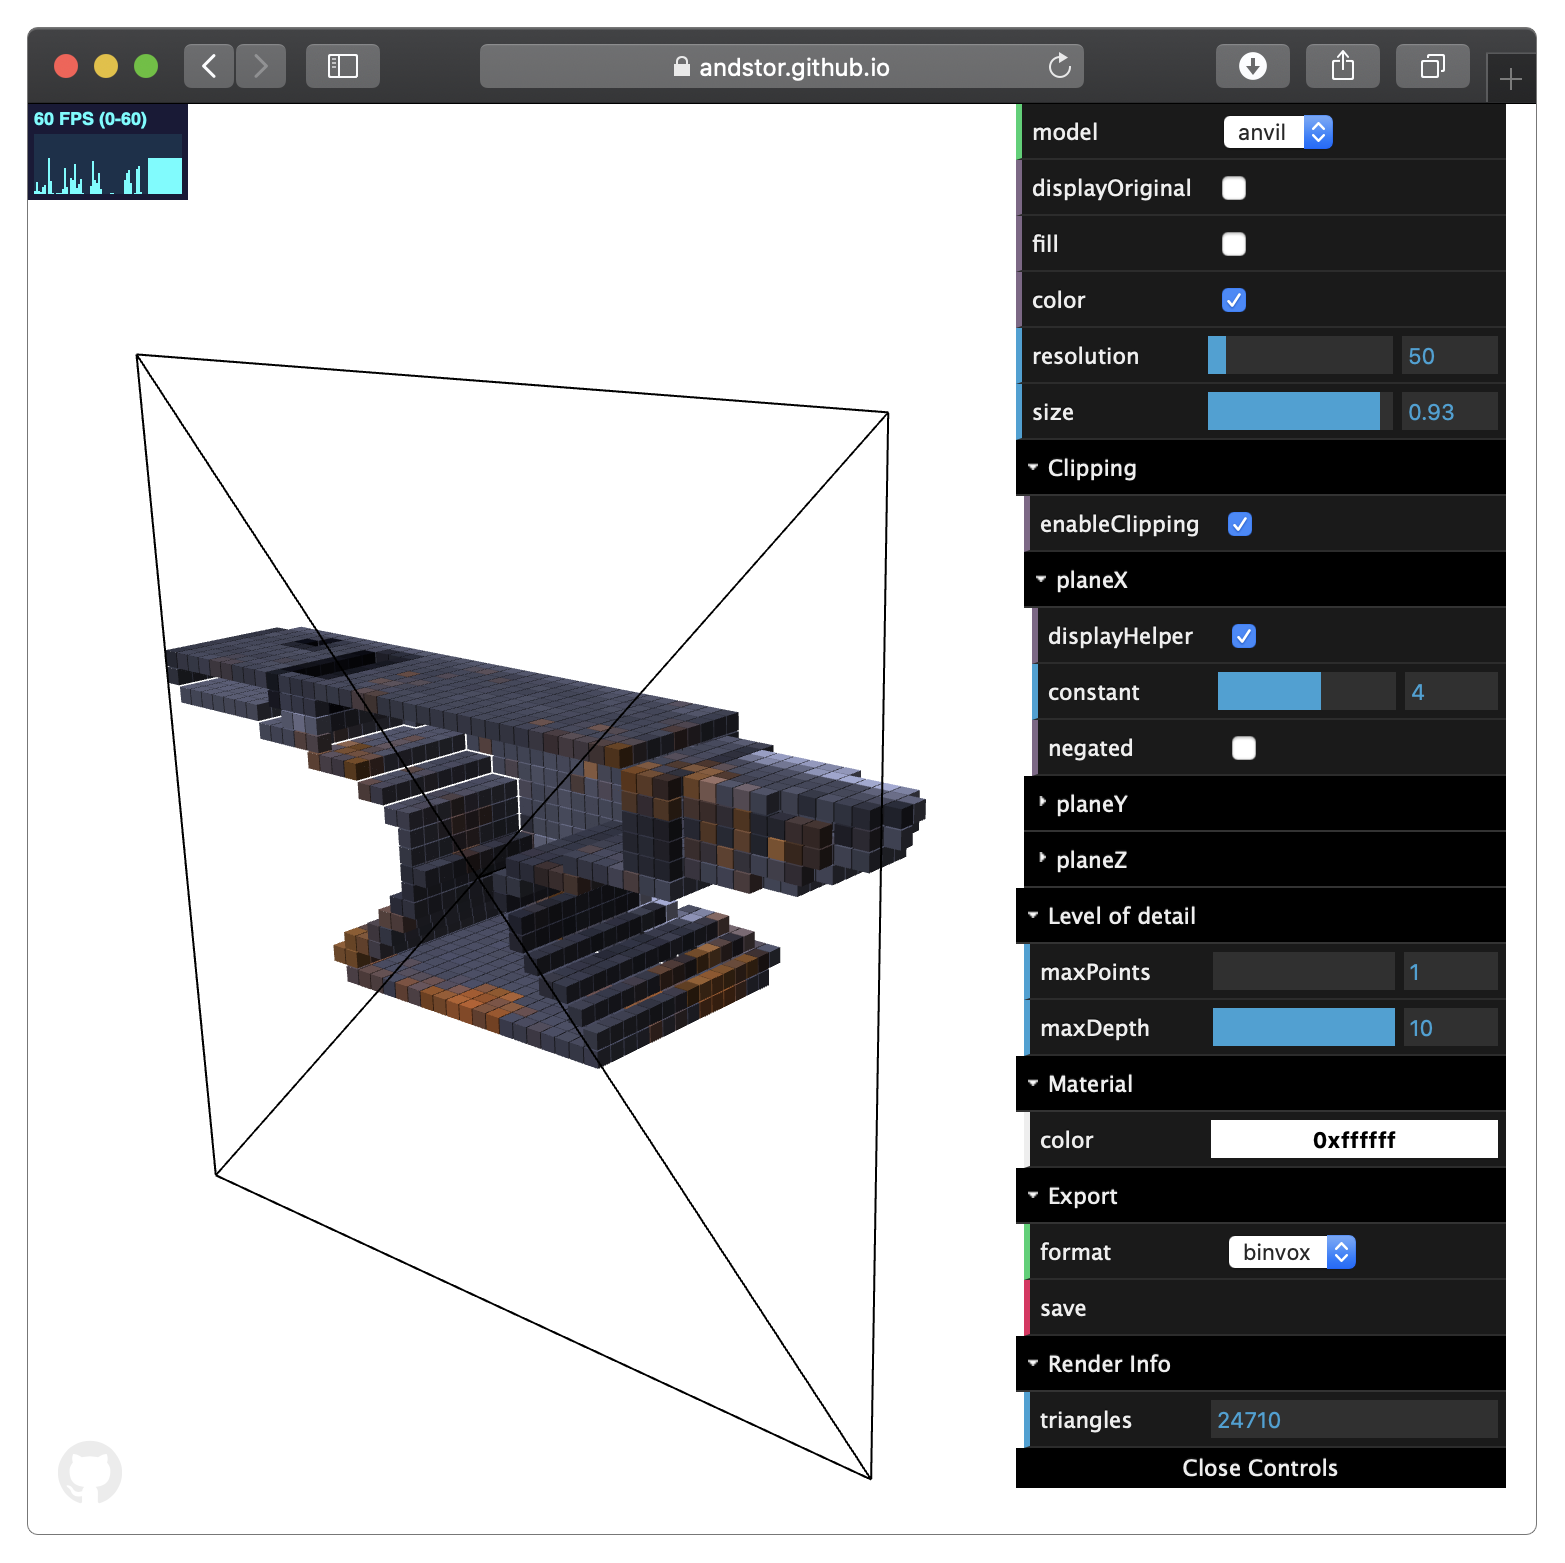
\includegraphics[width=0.9\textwidth]{sections/result/figures/voxelizer-example.png}
    \caption{Screenshot of the Voxelizer engine example page at GitHub Pages.}
    \label{fig:voxelizer-example}
\end{figure}

\subsection{Usage example}
Example walkthrough of how to use the library with code.
Like the one done for the JSDoc Action further down.

\lstinputlisting[language=JavaScript,style=numbers]{sections/methodology/code/voxelizer.js}

\section{BINVOX}
BINVOX is a package for parsing and building BINVOX files. It is published to the npm registry under the name "binvox", and the source code is available at GitHub under "andstor/binvox".

The package handles BINVOX files according to the BINVOX file format specification~\cite{binvox-file-format}. The package able to parse a BINVOX resource, turning it into JSON. Further, it can do this in reverse. Hence, properly formatted JSON data can be turned into a BINVOX file resource. The package provides both an ES Module build and a UMB build. It can therefore be used with both Node.js and in the browser.

\section{Voxelizer Desktop}
The Voxelizer Desktop application allows for easy use of the Voxelizer engine. It is a standalone cross platform desktop application. Ready-made installation files for macOS, Windows and Linux can be found at \url{https://github.com/andstor/voxelizer-desktop/releases/latest} on GitHub.

\subsection{Features}
The Voxelizer Desktop application includes several features.
\begin{itemize}
    \item \textbf{Importing} - The application supports several 3D model file formats. This includes GLB, GLTF, OBJ and STL. Some data formats need additional resources like texture images or binaries in order to work. This is also supported.
    \item \textbf{Voxelization} - The Voxelizer engine provides the application with voxelization capabilities. Several voxelization options are available, including: resolution, coloring and filling.
    \item \textbf{Visualization} - It is possible to view and inspect both the loaded 3D model and voxelized result through an interactive window.
    \item \textbf{Exporting} - Voxelizer Desktop enables the user to export to a XML file or a BINVOX file, and save this to the file system.
    \item \textbf{Auto updating} - When a new version of the application is released on GitHub, the application will automatically download and install the new version.
\end{itemize}

\subsection{GUI}
The user is first presented with an elegant and easy drag and drop user interface. Here, the user can just drop the 3D model files. Figure~\ref{fig:voxelizer-desktop-gui-dnd} shows a screenshot of the start screen, where a file is dropped onto the window.
\begin{figure}[htp]
    \centering
    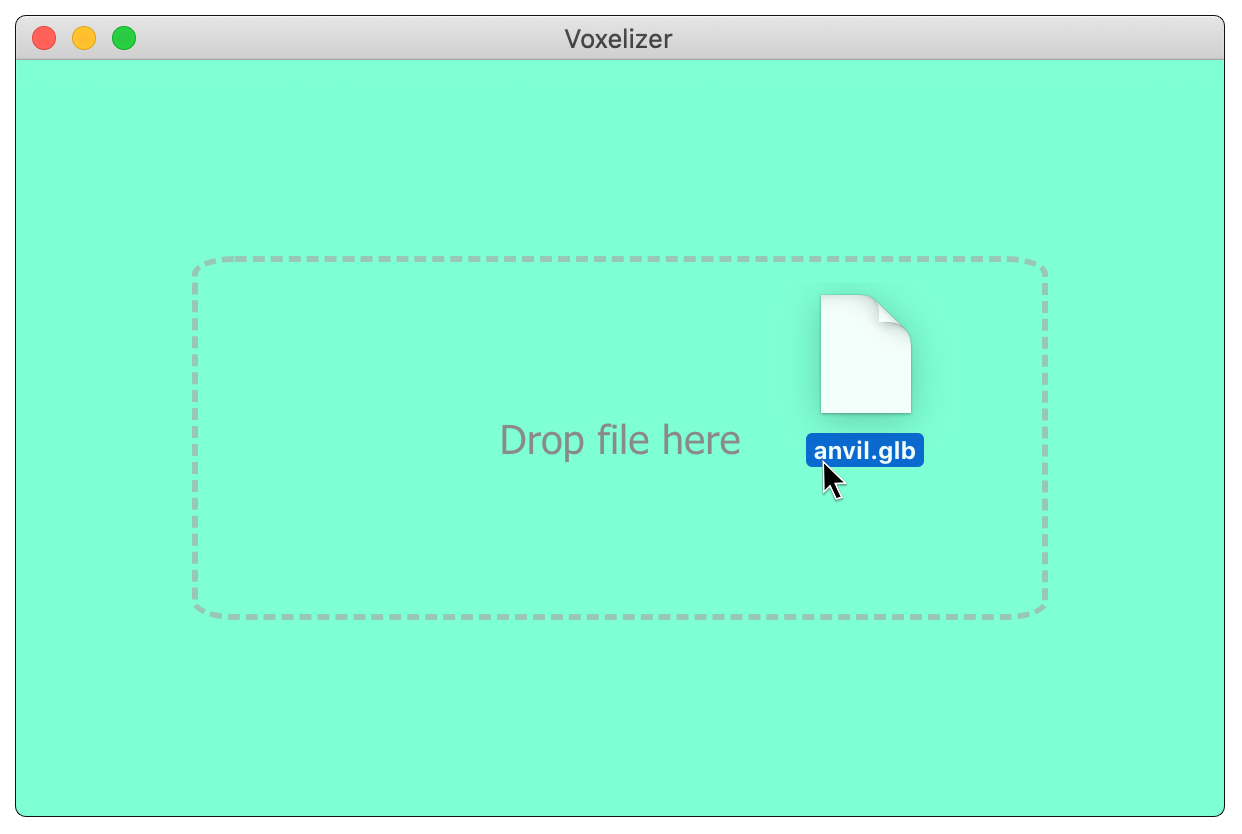
\includegraphics[width=0.9\textwidth]{sections/result/figures/voxelizer-desktop-gui-dnd.png}
    \caption{Voxelizer Desktop drag and drop start screen.}
    \label{fig:voxelizer-desktop-gui-dnd}
\end{figure}

When a user drops one or more files, the application starts to load them up. If no supported filetype is found, an modal warning shows up like the one seen in Figure~\ref{fig:voxelizer-desktop-gui-dnd-file-warning}. Otherwise, a spinning loading wheel is presented, as shown in Figure~\ref{fig:voxelizer-desktop-gui-loading}, to indicate that the 3D model is loading.

\begin{figure}[htp]
    \centering
    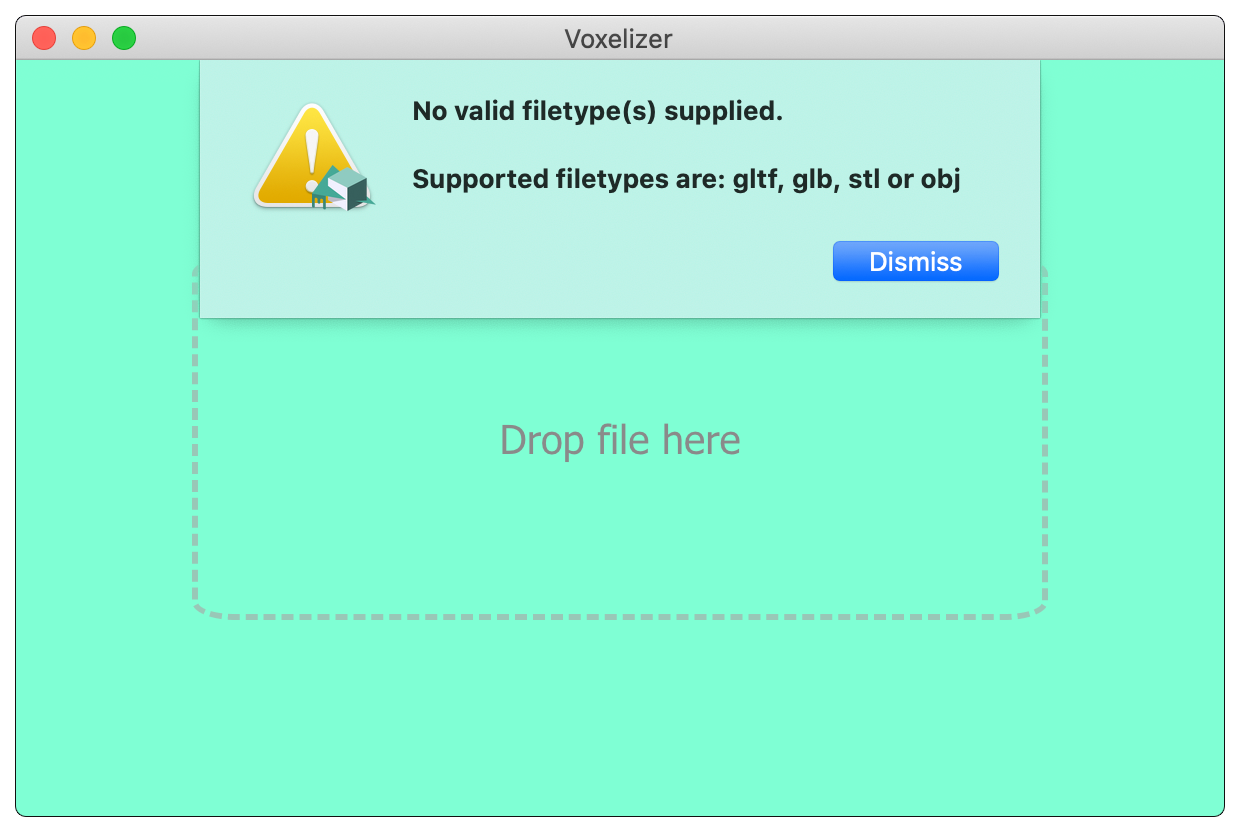
\includegraphics[width=0.9\textwidth]{sections/result/figures/voxelizer-desktop-gui-dnd-file-warning.png}
    \caption{Voxelizer Desktop drag and drop start screen filetype error.}
    \label{fig:voxelizer-desktop-gui-dnd-file-warning}
\end{figure}
\begin{figure}[htp]
    \centering
    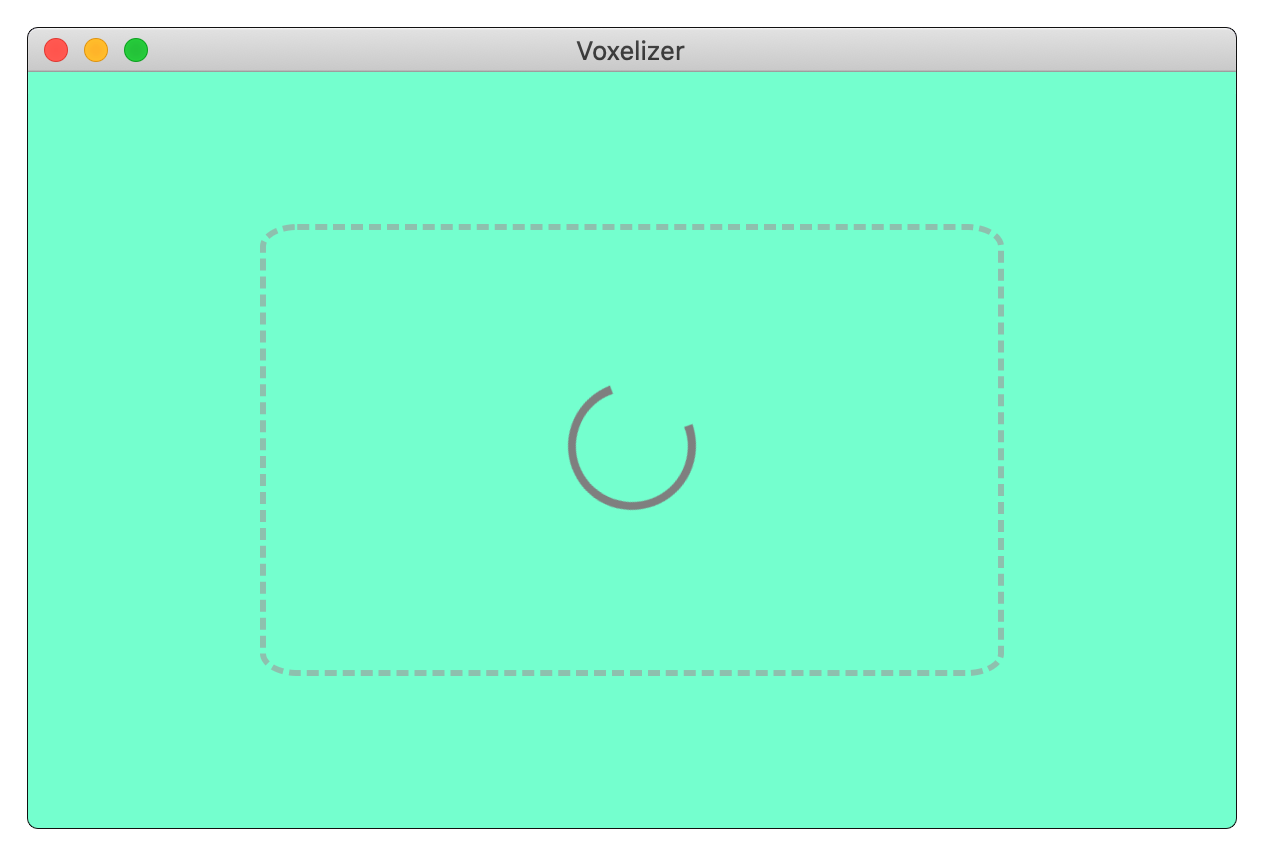
\includegraphics[width=0.9\textwidth]{sections/result/figures/voxelizer-desktop-gui-loading.png}
    \caption{Voxelizer Desktop loading 3D model.}
    \label{fig:voxelizer-desktop-gui-loading}
\end{figure}
\clearpage

When the loading finishes, the user is presented with the main interface. This is shown in Figure~\ref{fig:voxelizer-desktop-gui-main-light}. Here, the loaded 3D model is first presented in an interactive display. Further, at the bottom is various controls for the voxelization and for exporting.
\begin{figure}[htp]
    \centering
    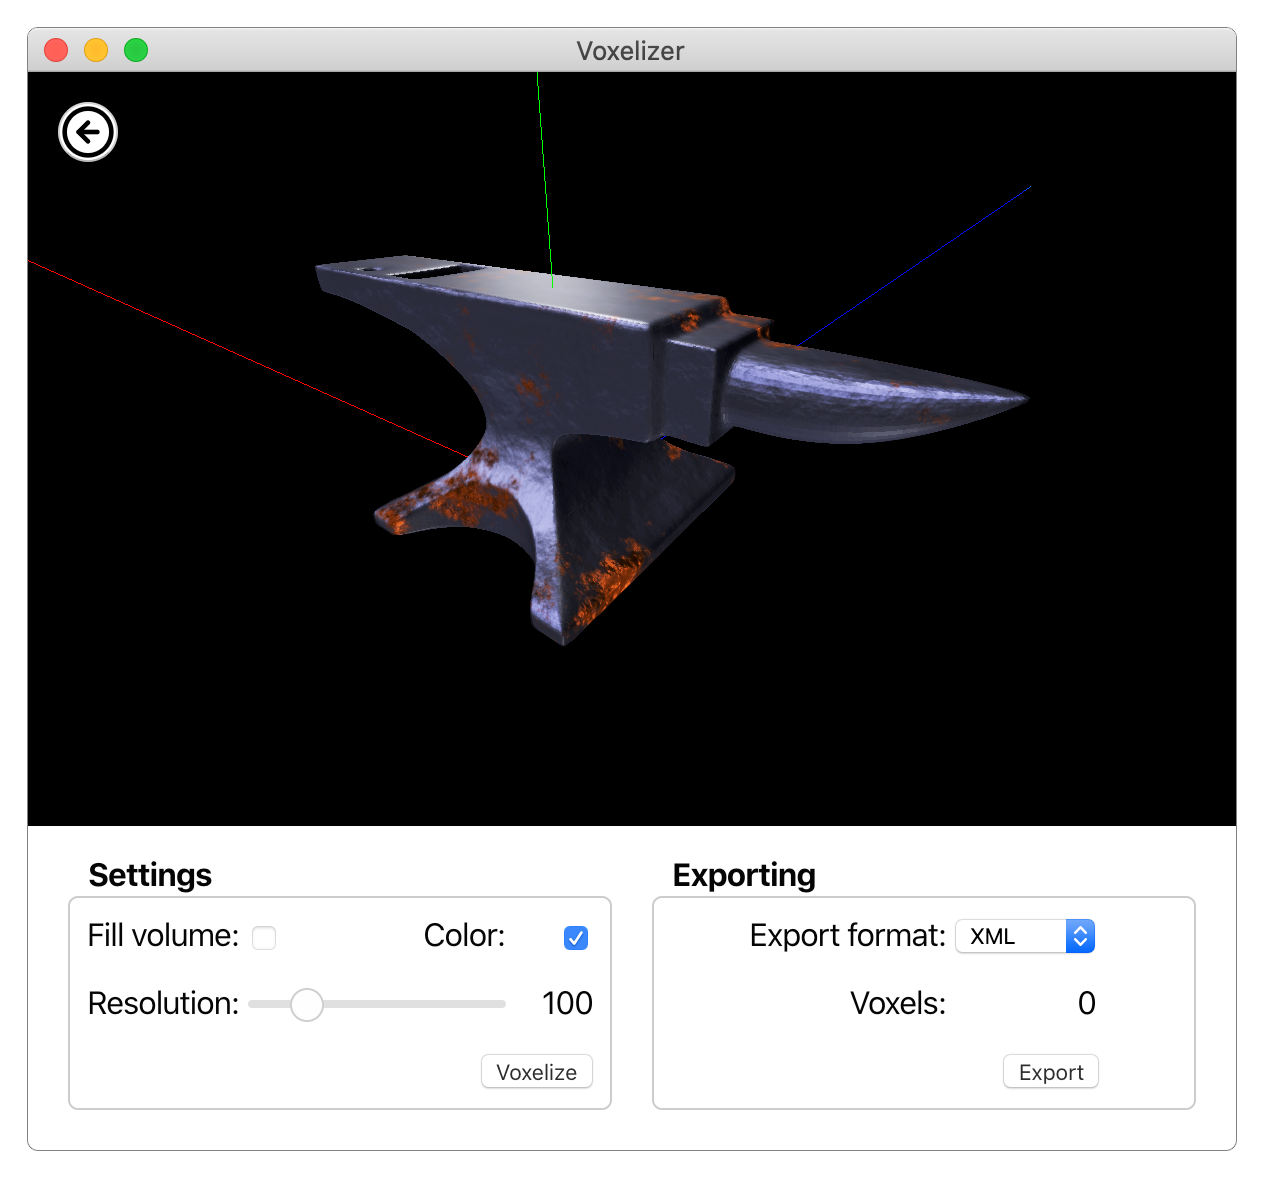
\includegraphics[width=0.9\textwidth]{sections/result/figures/voxelizer-desktop-gui-main-light.png}
    \caption{Voxelizer Desktop main interface.}
    \label{fig:voxelizer-desktop-gui-main-light}
\end{figure}
\clearpage

The application has support for dark mode. Meaning, depending on the system settings, either a light-theme or a dark-theme is selected. The application also has localization support (language). Currently, English and Norwegian Bokmål is available. The selected language will depend on the system settings. Figure~\ref{fig:voxelizer-desktop-gui-main-dark} shows the main interface in dark mode and with a Norwegian interface.
\begin{figure}[htp]
    \centering
    \includegraphics[width=0.9\textwidth]{sections/result/figures/voxelizer-desktop-gui-main-dark.png}
    \caption{Voxelizer Desktop with dark mode and Norwegian language.}
    \label{fig:voxelizer-desktop-gui-main-dark}
\end{figure}
\clearpage

If one tries to export before voxelizing the model, a modal will show a warning message. Figure~\ref{fig:voxelizer-desktop-gui-main-voxel-warning} shows this error message.
\begin{figure}[htp]
    \centering
    \includegraphics[width=0.9\textwidth]{sections/result/figures/voxelizer-desktop-gui-main-voxel-warning.png}
    \caption{Voxelizer Desktop voxel warning.}
    \label{fig:voxelizer-desktop-gui-main-voxel-warning}
\end{figure}
\clearpage

To actually voxelize the model, the user needs to click on the \textbf{Voxelize} button. This starts the voxelization process. When finished, the result is presented in the 3D graphics window. This can be seen in Figure~\ref{fig:voxelizer-desktop-gui-voxels}
\begin{figure}[htp]
    \centering
    \includegraphics[width=0.9\textwidth]{sections/result/figures/voxelizer-desktop-gui-voxels.png}
    \caption{Voxelizer Desktop displaying voxelized result.}
    \label{fig:voxelizer-desktop-gui-voxels}
\end{figure}
\clearpage

To export and save the voxel data in the selected file format, the user needs to click on the \textbf{Export} button. This opens up the operating system's file system dialog, as can be seen in Figure~\ref{fig:voxelizer-desktop-gui-export}. A file name and location then needs to be selected. When the user clicks on the \textbf{Save} button, the file is saved.
\begin{figure}[htp]
    \centering
    \includegraphics[width=0.9\textwidth]{sections/result/figures/voxelizer-desktop-gui-export.png}
    \caption{Voxelizer Desktop OS file dialog for saving voxel data.}
    \label{fig:voxelizer-desktop-gui-export}
\end{figure}

In order to voxelize a different 3D model, the user can click on the arrow icon in the upper left corner. When the user exits the application, the application state is saved. Among other things, this enables the application window to remember its window location and size.

\section{JSDoc Action}
\label{sec:result-jsdoc-action}
The JSDoc Action makes it easy to automate the process of generating JSDoc documentation. It is a GitHub Action, and is published to the GitHub Marketplace. Figure~\ref{fig:jsdoc-action-logo} shows the graphics generated by the GitHub Marketplace for the JSDoc Action. The source code is available at GitHub under "andstor/jsdoc-action".
\begin{figure}[htp]
    \centering
    \includegraphics[width=0.75\textwidth]{sections/result/figures/jsdoc-action-logo.png}
    \caption{Graphics from the GitHub Marketplace for the JSDoc Action.}
    \label{fig:jsdoc-action-logo}
\end{figure}

The action is easy to combine with other deployment actions. This makes it very simple to publish the generated documentation to any hosting service, for example GitHub Pages. The JSDoc Action also supports templates. These are installed with npm, so any package can be used. See the npm documentation for more details on the installation command~\cite{npm-install-docs}.

All that is needed for a minimum base setup is a workflow step like the one defined in Listing~\ref{lst:jsdoc-action-workflowstep}. This will generate documentation for all source files in the ./src directory, and output the built files to a ./out directory. Any other GitHub Action might further process this output.
\begin{lstlisting}[language=yaml,caption={Basic JSDoc Action workflow step},label={lst:jsdoc-action-workflowstep}]
- name: Build docs
  uses: andstor/jsdoc-action@v1
  with:
    source_dir: ./src
    recurse: true
    output_dir: ./out
\end{lstlisting}

\subsection{Example usage}
Following is a complete example of how easy it is to automate the JSDoc documentation process with the JSDoc Action. This assumes that GitHub is used for hosting the code to generate documentation for.

First, a workflow yaml file needs to be created. This file needs a name, say \textbf{documentation.yaml}, and has to be uploaded to the default branch in the user's repository, under ".github/workflows/". Then, the actual workflow needs to be defined. Listing~\ref{lst:jsdoc-workflow-deploy-example} provides an example workflow. This workflow is set to only run when code is pushed to the master branch. Ubuntu is then chosen as the platform to run the workflow job on. Several workflow steps are then defined:
\begin{enumerate}
    \item First, the user's code repository is cloned with the help of the Checkout Action by GitHub. This makes the user's source code available to subsequent steps. 
    \item Second, the JSDoc Action is used for generating the actual JSDoc documentation files. Lines 15-19 defines several input options to the JSDoc Action. The source directory is set to "./src". The output directory is set to "./out". A path to a JSDoc configuration file in the user's repository is then specified. In order to freshen up the plain JSDoc theme, the minami template is used. This is the name of the package on npm. Finally, the README.md file in the user's repository is used as frontpage. 
    \item Third, the GitHub Pages action is used for deploying the generated documentation files to GitHub Pages. It needs two input configurations. One is a deployment key. See the documentation for the GitHub Pages action for how to set up this. The other is a directory to get the files to publish. This is set to the the JSDoc Action's output directory, "./out".
\end{enumerate}

INCLUDE EXAMPLE SCREENSHOT OF HTML PAGE WITH GENERATED DOCS

%\begin{minipage}{\linewidth}
\lstinputlisting[language=yaml,style=numbers,label={lst:jsdoc-workflow-deploy-example},caption={Example documentation workflow file}]{sections/result/code/documentation-workflow.yaml}
%\end{minipage}
%\clearpage


\section{file-existence-action}
The File Existence action is a GitHub Action. The action is published to the GitHub Marketplace by the name "File Existence", and the source code is available at GitHub under "andstor/file-existence-action".

The action is able to check if one or more files exists during a workflow run. The user just supplies the paths as inputs to the action. The action then produces a boolean output variable which is available to the subsequent workflow steps. If any files are missing, the output is set to false. Otherwise, true. It is also possible to make the action trigger an error if one or more files are missing. This will effectively cancel the entire workflow.

\section{file-reader-action}
The File Reader action is a GitHub Action. The action is published to the GitHub Marketplace by the name "File Reader", and the source code is available at GitHub under "andstor/file-reader-action".

By providing a path as input to the action, the action is simply able to read the contents of a file during a workflow run. The action produces an output variable with the contents of the file. This variable will be available to the subsequent workflow steps.

\section{Automation}
More or less fully automated all build and release/publishing steps.
MORE HERE.... Describe how easy it is to maintain the various repositories!!!Include some screenshots from the GitHUb interface.

\subsection{JavaScript packages}
- Building
- Testing
- coverage upload to coveralls
- Security analysis with LGTM
- JavaScript documentation Generation and deployment of the docs to GH pages.
- Publishing module to NPM.

\subsection{GitHub Actions}
- automatic update of major version tags according to guidelines recommended by GitHub.


\section{Open-source community}
Several of the projects has already gained interest by the public. Say something about popularity....
Promotion of JSDoc Action in the main repo with 38 thousand users. ...more intro....

\subsection{Statistics}
Number of stars, weekly downloads, etc
MORE HERE...... Include screenshots of graphs etc...

\subsection{Feedback}
Several filed issues (which has been resolved). Feedback from the users, etc... Feature requests...

Included in MAIN JSDOC REPO!!! 10.000 stars and 38.000 users!!!

Supports templates and all that JSDoc3 natively supports.
Can use other actions to deploy docs to arbitrary service.
%This is chapter 5
%%=========================================
\chapter{Discussion}
This chapter discusses the achieved results, the execution of methodologies, and how the projects could be further improved. The chapter starts with Section~\ref{sec:discussion-requirements-scesification} that discusses the completeness of the entire project, compared to the requirements specification. Section~\ref{sec:discussion-working-methodology} describes how the chosen working methodology worked out. The improvements of the Voxelizer engine are discussed in Section~\ref{sec:discussion-voxelizer}, closely followed by the Voxelizer desktop application in Section~\ref{sec:discussion-voxelizer-desktop}. The level of automation achieved is described in Section~\ref{sec:discussion-automation}. The rest of the supportive projects are discussed in Section~\ref{sec:discussion-supportive-projects}. Finally, Section~\ref{sec:discussion-future-work} discusses some features that are left as future work.

\section{Requirements specification completeness}
\label{sec:discussion-requirements-scesification}
Most of the primary objectives are completed according to the requirement specification. Also, the majority of the user-stories are addressed, as can be seen from the backlog included in Appendix~\ref{appendix:backlog}. The project is therefore overall considered a success.

Due to various extra work like the binvox package, the file-existence-action and the file-reader-action, some functionality had to give way to others. It was not enough time to make the CLI tool for the Voxelizer engine. However, this could be a valuable companion tool for the Voxelizer engine, and should therefore be considered for future work.

\section{Working methodology}
\label{sec:discussion-working-methodology}
Scrum was used as the working methodology for this project. However, since Scrum is designed for teams, the method needed some adaptations. The changes described in Section~\ref{sec:method-scrum} worked out very well. The method helped in keeping the project on track. Further, the desire to complete the sprints functioned as a strong motivator throughout the entire project. This is backed by the sprint cumulative flow diagram available in Appendix~\ref{appendix:sprints}. The diagram shows a reasonable steady stream of completed issues throughout the entire project.

\section{Voxelizer}
\label{sec:discussion-voxelizer}
Compared to the old Voxelizer engine, the new version produces voxelization results of a lot higher quality. The improvement can clearly be seen from the results described in Section~\ref{sec:method-visual-assesment}. The engine is also greatly improved in terms of performance. Although, the level of performance gain shown in Section~\ref{sec:result-voxelizer-performance} was not expected, especially the huge reduction in memory footprint. Further, several new features are introduced. Being able to produce shell and color voxelizations makes the engine much more attractive.

During development, it became clear that extending the importing support for the different formats specified in the requirements specification was not beneficial. three.js already provides support for around 40 file formats. However, at the time of the creation of the old engine version, the loaders were hard to import and use. Since then, these loaders have implemented support for ES Modules. It was therefore decided that the task of loading the models should be left up to the user.

\section{Voxelizer Desktop}
\label{sec:discussion-voxelizer-desktop}
The Voxelizer Desktop ensures easy use of the Voxelizer engine. It fulfills all the main requirements. The application provides an intuitive user interface, and the voxelization process is very easy. By supporting several of the most popular 3D file formats, like OBJ, GLTF and STL, the user is most likely able to voxelize his/her files directly, without additional conversion steps.

\section{Automation}
\label{sec:discussion-automation}
The different projects were highly automated at an early stage. This made the various maintenance task throughout the project very easy. Future support and maintenance is therefore also expected be easy. Especially valuable is the JSDoc action. This will ensure available and up-to-date high-quality API documentation.

\section{Supportive projects}
\label{sec:discussion-supportive-projects}
Several tools were main to aid the various projects. This includes the three-voxel-loader plugin, the BINVOX package, the File Existence action and the File Reader action. With the exception of the three-voxel-loader, these tools are mainly the result of refactoring. Keeping the code in smaller modules, or packages, makes it easier to maintain. It also makes it easy for others to use the software for other projects. Further, this often means an increase in both testing and contributions to the project.

The three-voxel-loader three.js plugin proved to be very valuable in terms of testing. Inspecting the raw voxel data is more or less impossible. By visualizing the voxelized results, testing and debugging the Voxelizer engine was very easy.

\section{Future work}
\label{sec:discussion-future-work}
The uncompleted requirements specification and the user-stories provides an excellent basis for future work. In addition to this, the following sections suggests some additional improvements.

\subsection{three-voxel-loader}
The three-voxel-loader plugin generates a cube (CubeBufferGeometry) for every voxel. Even for voxels that are not visible from outside the model. When loading a large and filled voxel model, this results in an enormous number of faces being rendered, putting a heavy load on the hardware. A future improvement could be to only render an extracted surface mesh of the voxels result, when a voxel size of 1 is used. This would dramatically reduce the number of triangles needed to render the voxel model.

Another interesting feature could be to support isosurface extraction. This is the opposite process of the voxelization process. It tries to approximate a 3D mesh directly based on voxel data. The most popular isosurface extraction algorithm is the the marching cube algorithm, published in 1987 by \citet{marching-cubes-cline-lorentsen}. Including this feature into the project could be of great value.

\subsection{Voxelizer}
Due to the fact that JavaScript is single-threaded, no multithreading is implemented in the Voxelizer Engine. However, it is possible to implement a sort of multithreading with Web Workers in the browser, or Worker Threads in Node.js. A future improvement could be to implementing support for this type of multithreading directly into the Voxelizer engine. This way, the heavy voxelization calculations could be split up into chunks and voxelized in parallel.

%This is chapter 6
%%=========================================
\chapter{Conclusion}
The project is overall considered a success. A primary objective of this thesis was to improve the Voxelizer engine. The engine is completely overhauled, addressing all known issues with the old version. Several new features are also added, like coloring and shell voxelization. The performance of the engine is also greatly improved. The speed of the voxelization is significantly increased, and the memory footprint is reduced by several orders of magnitudes. The exporting capabilities are also extended with several file formats and data structures. This includes ndarrays, XML, and BINVOX. Exporting to BINVOX files is made possible with the new BINVOX JavaScript package.

To make voxelization easy and accessible, a complementary cross platform desktop application is developed for the Voxelizer engine. This features a sleek drag and drop interface, along with visualized voxelization results, made able with the new three-voxel-loader three.js plugin.

To ensure the projects keep a high level of quality, and are easy to maintain, a lot of automation is implemented. This has removed much of manual and laborious work. It has also made the software a lot safer, drastically reducing the potential of human errors and bug introductions. To achieve this level of automation, several GitHub Actions are developed. This mainly includes the highly successful documentation tool, the JSDoc Action. It is embraced by the popular JSDoc tool, and is already gaining in popularity. Two more actions are also developed for automation purposes. This is the File Existence action, and the File Reader action.   

To summarize, the Voxelizer engine is greatly improved, and a complementary desktop application is developed. Alongside, several automation tools are created and used in the projects.
%%===================================
\printbibliography
%This is an Appendix
%%=========================================

\appendix
\chapter*{Appendices}
\addcontentsline{toc}{chapter}{Appendices}
%\renewcommand{\thesection}{\Alph{section}}

\subimport{appendices/}{appendix-a}
\subimport{appendices/}{appendix-b.tex}
\subimport{appendices/}{appendix-c.tex}
\end{document}
